%% LyX 2.1.3 created this file.  For more info, see http://www.lyx.org/.
%% Do not edit unless you really know what you are doing.
\documentclass[12pt,oneside,english,reqno]{amsbook}
\renewcommand{\familydefault}{\rmdefault}
\usepackage[T1]{fontenc}

\usepackage{geometry}
\geometry{verbose,tmargin=1in,bmargin=1in,lmargin=1in,rmargin=1in}
\usepackage{mathrsfs}
\usepackage{url}
\usepackage{amsbsy,latexsym,amsmath}
\usepackage{amsfonts}
\usepackage{amssymb}
\usepackage[mathscr]{eucal}
\usepackage{epsfig,graphics,graphicx}
\usepackage{color}
\usepackage{amsthm}
\usepackage{amstext}
\usepackage{stmaryrd}
\usepackage{graphicx}
\usepackage{setspace}
\doublespacing

\makeatletter

%%%%%%%%%%%%%%%%%%%%%%%%%%%%%% LyX specific LaTeX commands.
%% A simple dot to overcome graphicx limitations
\newcommand{\lyxdot}{.}
%%%%%%%
\newtheorem{lemma}{Lemma}

 \newcommand{\abs}[1]{\left|{#1}\right|}
 \newcommand{\av}[1]{\left\langle #1 \right\rangle}
 
  \newcommand{\br}[1]{\langle #1|}
  \newcommand{\ke}[1]{|#1\rangle}
  \newcommand{\bk}[2]{\langle #1|#2\rangle}
  \newcommand{\kb}[2]{\ke{#1}\br{#2}}
  \newcommand{\var}[2]{\langle #1,#2\rangle} 
  
  \newcommand{\al}[1]{^{(#1)}}
  \newcommand{\da}{^\dagger} 
  
  \newcommand{\pt}[1]{\left( #1 \right)}
  \newcommand{\pq}[1]{\left[ #1 \right]}
  \newcommand{\pg}[1]{\left\{ #1 \right\}} 
  
  \newcommand{\lpt}[1]{\left( #1 \right.}
  \newcommand{\lpq}[1]{\left[ #1 \right.]}
  \newcommand{\lpg}[1]{\left\{ #1 \right.}
  \newcommand{\rpt}[1]{\left. #1 \right)}
  \newcommand{\rpq}[1]{\left. #1 \right]}
  \newcommand{\rpg}[1]{\left. #1 \right\}} 


\newcommand{\td}[1]{\widetilde{#1}}

%%%%%%%%%%%%%%%%%%%%%%%%%%%%%% Textclass specific LaTeX commands.
\numberwithin{section}{chapter}
\numberwithin{equation}{section}
\numberwithin{figure}{section}

\makeatother

\usepackage{babel}

\begin{document}


\global\long\def\sandwich#1#2#3{ \left\langle #1\left|#2\right|#3\right\rangle }
\global\long\def\ket#1{\left|#1\right>}
\global\long\def\braket#1#2{\left\langle #1\mid#2\right\rangle }
\global\long\def\bra#1{\left\langle #1\right|}
\global\long\def\indep{\perp\!\!\!\perp}




 \thispagestyle{empty}\pagenumbering{gobble}

\vphantom{}

\textbf{\large{}Quantum State Discrimination and Quantum Cloning: }{\large \par}

\textbf{\large{}\hspace{2.7cm}Optimization and Implementation }{\large \par}

\vspace{1.2cm}


{\huge{}\hspace{5cm}\hspace{1cm}\hspace{1cm}}by

\vspace{0.7cm}


{\huge{}\hspace{5cm}\hspace{1.1cm}}Lazy bum

\vfill{}


\begin{singlespace}
A dissertation submitted to the Graduate Faculty in Physics in partial
fulfillment of the requirements for the degree of Doctor of Philosophy,
The City University of New York 
\end{singlespace}

\begin{center}
2015
\par\end{center}

\pagebreak{}

 \pagenumbering{roman}\setcounter{page}{2}\vphantom{}

\begin{singlespace}
\begin{center}
\vfill{}

\par\end{center}

%\begin{center}
%\includegraphics[width=2cm]{../ugur_dissertation_copy/img/creative_commons_logo_by}
%\par\end{center}

\begin{center}
2015\\
Undeserving lazy bum\\
Some rights reserved.\\
This work is licensed under a Creative Commons\\
Attribution 4.0 United States License.\\
\url{http://creativecommons.org/licenses/by/4.0/}
\par\end{center}
\end{singlespace}

\pagebreak{}

\vphantom{}

\vfill{}


\begin{center}
\begin{minipage}[c][1\totalheight][t]{1\columnwidth}%
\begin{singlespace}
\begin{center}
This manuscript has been read and accepted for the\\
Graduate Faculty in Physics in satisfaction of the \\
dissertation requirement for the degree of Doctor of Philosophy.
\par\end{center}\end{singlespace}
%
\end{minipage}
\par\end{center}

\vspace{3cm}


\begin{minipage}[t]{0.25\columnwidth}%
\begin{singlespace}
\rule[0.5ex]{1\columnwidth}{1pt}

Date\end{singlespace}
%
\end{minipage} \hfill{}%
\begin{minipage}[t]{0.6\columnwidth}%
\begin{singlespace}
\rule[0.5ex]{1\columnwidth}{1pt}

Prof. J�nos A. Bergou

Chair of Examining Committee\end{singlespace}
%
\end{minipage}

\vspace{2cm}


\begin{minipage}[t]{0.25\columnwidth}%
\begin{singlespace}
\rule[0.5ex]{1\columnwidth}{1pt}

Date\end{singlespace}
%
\end{minipage} \hfill{}%
\begin{minipage}[t]{0.6\columnwidth}%
\begin{singlespace}
\rule[0.5ex]{1\columnwidth}{1pt}

Prof. Igor L. Kuskovsky

Executive Officer\end{singlespace}
%
\end{minipage}

\vspace{1.5cm}


\begin{center}
\begin{minipage}[t]{0.8\columnwidth}%
\begin{singlespace}
Supervisory Committee:

\vspace{1cm}


Prof. Mark Hillery\hfill{}

\vspace{1cm}


Prof. Steven Greenbaum\hfill{} 

\vspace{1cm}


Prof. Ed Feldman\hfill{}

\vspace{1cm}


Prof. Neepa T. Maitra\hfill{}\end{singlespace}
%
\end{minipage}
\par\end{center}

\vspace{0.5cm}


\begin{center}
THE CITY UNIVERSITY OF NEW YORK
\par\end{center}

\pagebreak{}

{\huge{}\hspace{5cm}\hspace{1.2cm}}\textbf{\Large{}Abstract}{\Large \par}

\vspace{1.5cm}


\textbf{\large{}Quantum State Discrimination and Quantum Cloning: }{\large \par}

\textbf{\large{}\hspace{2.7cm}Optimization and Implementation }{\large \par}

\vspace{1.2cm}


{\huge{}\hspace{5cm}\hspace{1cm}\hspace{1cm}}by

\vspace{0.7cm}


{\huge{}\hspace{5cm}\hspace{1.1cm}}Lazy Bum

\vspace{1cm}


\textbf{Advisor:}\textbf{\small{} }Janos A. Bergou

\vspace{1cm}

This thesis reflects works previously published by the author and materials 
hitherto unpublished on the subject of quantum information theory.  Particularly,
results in optimal discrimination, cloning, and separation of quantum states, 
and their relationships, are discussed.  Via Neumark's theorem \cite{Neumark}, 
our description of these unitary processes can be implemented with linear optical devices. 



{\huge{}\hspace{1.0cm}}\textbf{\Large{}}{\Large \par}

\vspace{1.5cm}

\vspace{1.2cm}

\chapter*{Acknowledgements}


\vspace{0.7cm}



\vspace{1cm}


THANKS BRUVS, MUCH LOVE!



\tableofcontents{}

\listoffigures


 \pagenumbering{arabic}\pagebreak{}

%%%%%%%%%%%%%%%%%%%%%%%%%%%%%%%%%%%%%%%%%%%%%%%%
%%%%%%%%%%%%%%%%%%%%%%%%%%%%%%%%%%%%%%%%%%%%%%%%
\chapter{Introduction}


\section{On Why Quantum Information Theory Is Interesting}

Quantum state discrimination is the theory by which a measurement
on a quantum system relates to the information gathered from that
system. This field is important for myriad applications in communication,
cryptography, and computation. It remains important to devise better
theoretical frameworks for these processes and to realize them experimentally.

To peform a measurement in a quantum mechanical system, we must look to its state.
The state of a quantum system contains all information about the system.
\cite{Chefles}. Given a mixture of different states, only orthogonal
states can be distinguished perfectly \cite{Higgins}. For non-orthogonal
states \cite{Chefles3}, optimum discrimination will depend on the
type of information we wish to obtain and on prior information that
we have. Depending on the type of results needed, several different
strategies exist.

The traditional measurement minimizes the chance of incorrectly identifying
the state \cite{Helstrom}. It is known as the Minimum Error (ME)
strategy. In this strategy the measurements aim to identify the most
prominent states, either pure \cite{Ban} or mixed \cite{Eldar,Chou}. It
was first experimentally tested by  Barnett and Riis \cite{Barnett}, and quantitatively tested for
nonorthogonal states by Clarke \textit{et al.}\cite{Clarke1}.

If the states to be distinguished are linearly independent it is possible
to construct a measurement that always correctly identifies the input
state but does not always give an answer, ie has a certain failure
rate. This strategy is called Unambiguous State Discrimination (UD)
and was introduced by Ivanovic \cite{Ivanovic}. The optimal solution
for two pure states and arbitrary a-priori probabilities was solved by
Jaeger and Shimony \cite{Jaeger}. The solution was later extended
to include symmetric pure states, three pure states, and other classes
of mixed states. UD experiments fist done by Huttner \textit{et al.}\cite{Huttner}. 
 Extended by Clarke \textit{et al.} to pure trine and tetrad states in two dimensions.\cite{Clarke2}. 
UD was experimentally verified for discriminating pure and mixed quantum states by Mohseni \textit{et al.} \cite{Mohseni}.

If the input states are not linearly independent it is not possible
to distingiush them perfectly, but it is possible to improve on the
error associated with the ME strategy. For this a more recent addition
to the measurement strategy ensemble was the Maximum Confidence (MC)
strategy\cite{Croke}. Here the idea of the Baye's rule is used to
maximize the chance of the appropriate detector clicking for its desired
state.  The experimental realization was suggested by Herzog and Benson \cite{HerzogImp}, and
done by Steudle \textit{et al.} \cite{Steudle}.

The MC strategy was a move in the direction of Intermediate (IM) strategies,
where both errors and failure are permissible for a specific measurement
goal. The IM scheme was introduced by Chefles and Barnett \cite{Chefles5}
where they found the lower bound on the combination of error and inconclusive
result for two pure states with equal prior probabilities. Later,
Fiur��ek and Je�ek \cite{Fiurasek} generalized this result for mixed
states.

Recently the two pure state IM problem was first solved by Sugimoto 
\textit{et al.} \cite{Sugimoto} using Semi-Definite Programming (SDP),
where a fixed error rate was used to obtain an analytical solution.
Then Bagan \textit{et al.} \cite{Bagan} solved the problem using
an operator transformation technique that reformulated the IM problem
into a ME problem with an extra optimization parameter. Herzog generalized
the SDP approach to include classes of mixed states to the realm of
IM analytic solutions \cite{Herzog,Herzog1}.


In this paper we solve the IM problem two different ways via a strategy first developed by Neumark \cite{Neumark}. 
Both solutions are important to our understanding of the problem.  First we describe a 
normalization that reduces the problem, like in \cite{Bagan}, to a ME problem with an
implicit degree of freedom, a fixed failure rate.  The main difference with the aforementioned paper is that we need not
redefine operators, only weights for the probabilities involved.  The second solution uses 
the method of a Lagrange multiplier and constrained failure rate to develop an explicit algebraic solution.  The
advantage of this solution is that is allows us to extract not only the total probabilities of success and
failure, as were derived previously, but individual probabilities for each state.

Thus the Neumark method is useful because it explicitly describes the action of a unitary transformation
on input states and correlates them with the output states and occurance probabilities thereof.
Because of this transparent approach to the problem, we can derive the unitary matrix
elements as functions of the probabilities of successfully and erroneously distinguishing the input states.  
We can design a linear optical experiment for actualizing this unitary by the methods described in \cite{Reck, Sun, BergouImp}.
Namely, we decompose the unitary into the action of three beamsplitters onto single degrees of freedom of a polarized beam
of photons.  As this method does not require more advanced experimentalist technology than has been implemented for the
realization of the UD experiments, we are confident that this theory can be readily verified.
 Are there other papers in the field
that are relevant?


Motivation to study the subsequent topics comes from a long list of achievements by physicists for the last hundred years.  The tenant
that all information is physical and therefore encoded in the states of  systems \cite{Andi2} allows us to consider optimal interactions with
quantum systems as generalized measurements on density matricies representing the states' configurations.  Because the state is not a 
directly observable quantity \cite{Andi3} we have a prescribed method of interacting with it.  Particularly the formulation due to Neumark
where 


Classical bits versus quantum bits: instead of just a 0 or 1, quantum bits can maintain a superposition state

The probabalistic nature of detection: only orthogonal states can be discriminated perfectly


Quantum Computing

Quantum Communication
 factorization work of Peter Schor \cite{Shor1994} and quantum
key distribution protocols such as B92 \cite{Bennett1992}. 

%%%%%%%%%%%%%%%%%%%%%%%%%%%%%%%%%%%%%%%%%%%%%%%%
%%%%%%%%%%%%%%%%%%%%%%%%%%%%%%%%%%%%%%%%%%%%%%%%
\section{State Representation and Measurements }

We begin by describing pure quantum states $\psi$ as vectors in a Hilbert space and an ensemble of states as
 $\rho  = \sum_i \eta_i \kb{\psi_ i}{\psi_i}$ where $\sum \eta_i = 1$. The evolution of this ensemble is the 
Schrodinger equation as
\[i \hbar \frac{\partial\rho}{\partial t} =  [H,\rho].\]
Solving this for evolution of initial state $\rho(t=0)$ we get
\[\rho(t) = U(t) \rho(0) U(t)^\dagger.\]
and where the unitary matrix U obeys $UU^\dagger = I$.
There are several ways to view this formula. The first is by decomposing the unitary into a set of Kraus operators $A_i$
such that $\sum A_i A_i^\dagger = I$.  This allows us to write the evolution of pure states interacting through unitary evolution as
\begin{equation}
U(\ke {\psi_A} \otimes \ke {\phi_B}) = \sum_i A_i \ke {\psi_A} \otimes \ke {i_B}.
\end{equation}
This equation describes the alternative effects of the evolution between states $\ke {\psi_A}$ and $\ke{\phi_B}$ in the space $H_1 \otimes H_2$ as a Kraus operator $A_i$ for each  outcome direction $\ke {i_B}$ of the ancilliary Hilbert space, such as a measurement device.  For example a particle striking 
one detector as opposed to another can be described by the different operators $A_i$.

The other is due to Neumark \cite{Neumark1}. A unitary acts on a pure state $\psi$ to make state $\phi$, as in $U\ke \psi = \ke \phi$.
Before we describe such processes particularly let us describe the mathematics of these structures.  The ensemble 
previously described can be describes as a density matrix.  This is a generalized state that is a statistical collection 
of pure states defined by four properties:

\begin{enumerate}
\item $\rho  = \sum_i \eta_i \kb{\psi_ i}{\psi_i}$ where $\sum \eta_i = 1$,
\item It is Hermitian,
\item $Tr \rho = 1$,
\item $\br {\phi_i} \rho \ke {\phi_i} \geq 0$.
\end{enumerate}

The Kaus operators can be associated with measurement operators $\Pi_i$ such that $\Pi_i = A^\dagger_i A_i$. Hence the $\Pi_i$ are a decomposition of the identity in terms of positive semi-definite matrices.  A measurement can be either a projector onto an eigenvector of the Hilbert space or a generalized measurement.  In the latter case it must fulfill only 2 properties:
\begin{enumerate}
\item $\sum \Pi_i = 1$
\item They are Hermitian.  This corresponds to real eigenvalues (measurement outcomes).
\end{enumerate}
Since non-orthogonal states cannot be discriminated perfectly, we can speak of the probability of a given outcome:
	$\av {\Pi_i} = \sum_j \eta_j \br {\psi_j} \Pi_i \ke {\psi_j} = Tr(\Pi_i \rho)$
This further justifies the motivation for the measurement operators. 



%%%%%%%%%%%%%%%%%%%%%%%%%%%%%%%%%%%%%%%%%%%%%%%%
%%%%%%%%%%%%%%%%%%%%%%%%%%%%%%%%%%%%%%%%%%%%%%%%%%%%%%%%%%%%%%%%%%%%%%%%%%%%%%%%%%%%%%%%%%%%%%%%
%%%%%%%%%%%%%%%%%%%%%%%%%%%%%%%%%%%%%%%%%%%%%%%%
\chapter{Discrimination of Pure States}
Consider the problem of discriminating between two states $\ke \psi_1$ and $\ke \psi_2$.  If we could always perform this perfectly
then we should be able to write a unitary U such that 
\begin{eqnarray}
U\ke {\psi_1}= \ke 1,\\
U\ke {\psi_2} = \ke 2,
\end{eqnarray}
where the states $\ke 1$ and $\ke 2$ are orthogonal in the basis of the input states, and each result is associated with the respective input.  However
since the unitary is inner-product preserving, taking the product of the first with the second's adjoint shows
this unitary and hence such a measurement are impossible unless the input states are orthogonal:
\[\br {\psi_2} U^\dagger U \ke {\psi_1} = \bk {\psi_2}{\psi_1} = \bk 1 2 = 0.  \]
We can make a similar demonstration
using the operator method.  If 
\begin{eqnarray}
\Pi_1 \ke {\psi_2} = 0, \\
\Pi_2 \ke {\psi_1} = 0,
\end{eqnarray} 
then using $\Pi_1 + \Pi_2 = I$ and inner product of these equations, we get the same result:
\[0= \br{\psi_2} \Pi_1 + \Pi_2 \ke {\psi_1} = \bk{\psi_1}{\psi_2} \]

 Since the two constraints of measurement,
orthogonality of the measurement vectors and their spanning the space, proved contradictory, we must give up one of these two
functions in order to perform a physical measurement.
 Hence we must choose a unitary that performs this task optimally according to some figure of merit, typically a probability measure.  For all future discussion
we assume that the input states $\psi_1$ and $\psi_2$ are provided one at a time, 
and with known probabilities $\eta_1$ and $\eta_2$ respectively, such that $\eta_1 + \eta_2 = 1$.  



%%%%%%%%%%%%%%%%%%%%%%%%%%%%%%%%%%%%%%%%%%%%%%%%
%%%%%%%%%%%%%%%%%%%%%%%%%%%%%%%%%%%%%%%%%%%%%%%%
\section{Minimum Error Discrimination}
Historically, the first solution to this problem is due to Helstrom \cite{Helstrom1969}.  
Now known as the Minimum Error (ME) strategy, the figure of merit is the average rate
of mistakingly identifying one state for the other.  Using the density matrix and trace notation,
this average probability of error can be written as
\[P_e = \eta_1 tr[\rho_1 \Pi_2] + \eta_2 tr[\rho_2 \Pi_1],\]
where we associate the outcome $\Pi_i$ with state $\psi_i$.
Analagously, the average probability of success is simply 
\[P_s = \eta_1 tr[\rho_1 \Pi_1] + \eta_2 tr[\rho_2 \Pi_2],\]
Because we want a result every time a state is sent to us the
operators $\Pi_i$ must span the space, so $\Pi_1 + \Pi_2 = I$ which implies $P_e + P_s =1$.  The minimum error is attained at the Helstrom bound:
\begin{equation}
P_{E}=\frac{1}{2}[1-\sqrt{1-4\eta_{1}\eta_{2}|\langle\psi_{1}|\psi_{2}\rangle|^{2}}].
\end{equation}
The detectors and states can are graphically represented in Fig. 1 for the case when the given states are qubits and occur with equal likelihood.

\begin{figure}
\begin{centering}
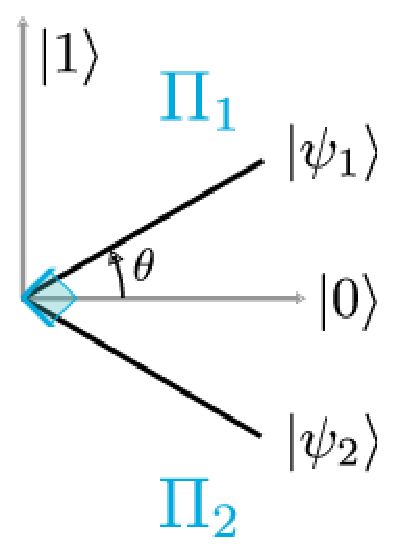
\includegraphics[width=8.5cm,height=8.5cm]{ME}\protect\caption[\hspace{1cm}Min Error]{ The states $\psi_i$ and projectors $\Pi_i = \kb {\phi_i}{\phi_i}$ which minimizes the error rate for detection.
along the states $\left\{ \protect\ket{\psi_{1}},\protect\ket{\psi_{2}}\right\} $
for $\eta_{1}=\eta_{2}=\frac{1}{2}$. }

\par\end{centering}

\label{POVM_ME} 
\end{figure}

We provide a derivation of this result to demonstrate the Neumark formalism.
Since both $\psi_1$ and $\psi_2$ can now evolve to either $0$ or $1$, we must write the unitary equations as
\begin{eqnarray}
U \ke{\psi_1} = \sqrt{p_1} \ke 1 + \sqrt{r_1} \ke 2\\
U \ke{\psi_2} = \sqrt{p_2} \ke 2 + \sqrt{r_2} \ke 1,\label{eq:ME neumark}
\end{eqnarray}
where $p_i$ and $r_i$ are the individual success and error probabilities of the measurement.  Taking the inner product of these 
two equations with themselves we find $p_i + r_i = 1$, and taking the inner product with each other we get the overlap constraint

\begin{equation}
s = \bk{\psi_1}{\psi_2} = \sqrt{p_1 r_2} + \sqrt{ p_2 r_1}, \label{eq:ME constraint}
\end{equation}

We wish to minimize the average error rate

\begin{equation}
P_{E}=\eta_{1}r_{1}+\eta_{2}r_{2},\label{eq:ME}
\end{equation}

subject to the constraint in (\ref{eq:ME constraint}).  We solve this two variable problem using the method of Lagrange multipliers.  
For details on this method see Appendix 2.  The constrained error equation can be written as

\begin{equation}
F(r_1,r_2,\lambda)=\eta_{1}r_{1}+\eta_{2}r_{2}+\lambda\left[s-\sqrt{(1-r_{1})r_{2}}-\sqrt{(1-r_{2})r_{1}}\right].
\end{equation}

Our extrema will be found when all partial derivatives of this equation are zero, therefore

\[
\frac{\partial F_{E}}{\partial r_{1}}=\eta_{1}+\frac{1}{2}\left[\sqrt{\frac{r_{2}}{1-r_{1}}}-\sqrt{\frac{1-r_{2}}{r_{1}}}\right]=0,
\]
and

\[
\frac{\partial F_{E}}{\partial r_{2}}=\eta_{2}+\frac{1}{2}\left[-\sqrt{\frac{r_{1}}{1-r_{2}}}+\sqrt{\frac{1-r_{1}}{r_{2}}}\right]=0.
\]

We notice that these two equations may be re-arranged such that the left hand side is dependent on a single variable:


\begin{equation}
\frac{2\eta_{1}}{\lambda}\sqrt{r_{1}(1-r_{1})}=\sqrt{r_{1}r_{2}}-\sqrt{(1-r_{1})(1-r_{2})},\label{eq:r12}
\end{equation}


\begin{equation}
\frac{2\eta_{2}}{\lambda}\sqrt{r_{2}(1-r_{2})}=\sqrt{r_{1}r_{2}}-\sqrt{(1-r_{1})(1-r_{2})}.\label{eq:r1r2}
\end{equation}


The right hand sides of Eq.(\ref{eq:r12}) and (\ref{eq:r1r2}) can
be set to a constant $\frac{2\eta_{i}}{\lambda}\sqrt{r_{i}(1-r_{i})}\equiv C$,
which can later be determined from the unitarity constraint \ref{eq:ME constraint}, 

\begin{eqnarray}
r_{i} & = & \frac{1}{2}\left(1\pm\sqrt{1-\frac{\lambda^{2}C^{2}}{\eta_{i}^{2}}}\right)=\frac{1}{2}\left(1-\sqrt{1-\frac{\delta^{2}}{\eta_{i}^{2}}}\right),\label{eq:r_i-1}\\
r_{i} & = & \frac{1}{2}\left[1-A_{i}\right],
\end{eqnarray}


where $A_{i}\equiv\sqrt{1-\frac{\delta^{2}}{\eta_{i}^{2}}}$ and $\delta^{2}\equiv\lambda^{2}C^{2}$.
The smaller $r_{i}$ is picked (lower sign in \ref{eq:r_i-1} ) as
this represents error rate, which is to be minimized. Now replace
$r_{i}$ into the constraint (\ref{eq:ME constraint}) and solve for
$\delta$:

\begin{eqnarray*}
s & = & \sqrt{(1-r_{1})r_{2}}+\sqrt{(1-r_{2})r_{1}},\\
2s & = & \sqrt{(1+A_{1})(1-A_{2})}+\sqrt{(1-A_{1})(1+A_{2})},\\
2s^{2} & = & 1-A_{1}A_{2}+\sqrt{(1-A_{1}^{2})(1-A_{2}^{2})},\\
2s^{2} & = & 1-A_{1}A_{2}+\frac{\delta^{2}}{\eta_{1}\eta_{2}},\\
(2s^{2}-1 & -\frac{\delta^{2}}{\eta_{1}\eta_{2}})^{2}= & 1-\frac{\delta^{2}}{\eta_{1}^{2}}-\frac{\delta^{2}}{\eta_{2}^{2}}+\frac{\delta^{4}}{\eta_{1}^{2}\eta_{2}^{2}}.
\end{eqnarray*}


After some tedious but trivial algebra:

\begin{equation}
\delta^{2}=\frac{4s^{2}(1-s^{2})\eta_{1}^{2}\eta_{2}^{2}}{1-4\eta_{1}\eta_{2}s^{2}}.\label{eq:delta}
\end{equation}


Now substitute the value of $\delta$ from (\ref{eq:delta}) into
(\ref{eq:r_i-1}) to get the explicit form of the individual error
rates,

\begin{equation}
r_{i}=\frac{1}{2}\left[1-\frac{1-2\eta_{i}s^{2}}{\sqrt{1-4\eta_{1}\eta_{2}s^{2}}}\right]
\end{equation}


Inserting $r_{1}$ and $r_{2}$ into (\ref{eq:P_E}) Helstrom bound
is retrieved \cite{Helstrom1969}

\begin{eqnarray}
P_{E} & = & \frac{1}{2}\left[1-\frac{\eta_{1}-2\eta_{1}\eta_{2}s^{2}}{\sqrt{1-4\eta_{1}\eta_{2}s^{2}}}-\frac{\eta_{2}-2\eta_{1}\eta_{2}s^{2}}{\sqrt{1-4\eta_{1}\eta_{2}s^{2}}}\right],\nonumber \\
P_{E} & = & \frac{1}{2}\left[1-\sqrt{1-4\eta_{1}\eta_{2}s^{2}}\right].
\end{eqnarray}

%%%%%%%%%%%%%%%%%%%%%%%%%%%%%%%%%%%%%%%%%%%%%%%%
%%%%%%%%%%%%%%%%%%%%%%%%%%%%%%%%%%%%%%%%%%%%%%%%
\section{Unambiguous Discrimination}

It was noticed by *UD CITations** that we may completely eliminate error from the measurement results
by giving up the constraint that our two measurement operators span the whole space, $\Pi_1 + \Pi_2 = I$.  This creates an additional result which 
is not associated with the state being either $\psi_1$ or $\psi_2$ .  It is called the inconclusive or failure outcome $\Pi_0$,
and the new decomposition of the identity reads $\Pi_0+ \Pi_1 + \Pi_2 = I$.  


\begin{eqnarray}
\Pi_{1} & = & \frac{p_{1}}{|\langle\psi_{1}|\psi_{2}^{\perp}\rangle|^{2}}|\psi_{2}^{\perp}\rangle\langle\psi_{2}^{\perp}|,\nonumber \\
\Pi_{2} & = & \frac{p_{2}}{|\langle\psi_{2}|\psi_{1}^{\perp}\rangle|^{2}}|\psi_{1}^{\perp}\rangle\langle\psi_{1}^{\perp}|.\label{eq:Pi1Pi2}
\end{eqnarray}


To determine the failure operator, insert (\ref{eq:Pi1Pi2}) into
(\ref{eq:3povms}): 

\begin{equation}
\Pi_{0}=I-\Pi_{1}-\Pi_{2}=I-\frac{p_{1}}{|\langle\psi_{1}|\psi_{2}^{\perp}\rangle|^{2}}|\psi_{2}^{\perp}\rangle\langle\psi_{2}^{\perp}|-\frac{p_{2}}{|\langle\psi_{2}|\psi_{1}^{\perp}\rangle|^{2}}|\psi_{1}^{\perp}\rangle\langle\psi_{1}^{\perp}|.
\end{equation}

The eigenvalues of $\Pi_{0}$ must be non-negative, giving us the inequality constraint between the individual failure rates as

\begin{equation}
q_{1}q_{2}\geq|\langle\psi_{1}|\psi_{2}\rangle|^{2}.\label{eq:qConstraint}
\end{equation}
 where we used $q_{i}=1-p_{i}.$

Now our value of merit will be the average failure rate $Q = \eta_1 q_1 + \eta_2 q_2$.  Since there is no error the success and failure
add to one: $P_s + Q = 1$.  Hence we wish to minimize the failure rate by taking the equality in Eq. (\ref{eq:qConstraint}), giving us the minimum
failure rate at
\begin{equation}
Q \equiv Q_0 = 2 \sqrt{\eta_1 \eta_2}|\langle\psi_{1}|\psi_{2}\rangle|. \label{Q0}
\end{equation}

This solution is valid for $q_{i}\leq1.$  Outside of this bound we ignore the state with the high rate of failure by removing that detector and
reducing our measurement strategy back to projective measurements.  We project onto the more likely state.  Therefore the total UD solution is
\begin{equation}
Q_{{\rm c}}=\left\{ \begin{array}{l}
\eta_{1}+\eta_{2}\cos^{2}\theta,\mbox{if \ensuremath{{\displaystyle \eta_{1}<\frac{\cos^{2}\theta}{1+\cos^{2}\theta}\equiv\eta_{1}^{(l)}}},}\\[0.7em]
\eta_{2}+\eta_{1}\cos^{2}\theta,\mbox{if \ensuremath{\eta_{1}>{\displaystyle \frac{1}{1+\cos^{2}\theta}\equiv\eta_{1}^{(r)}}},}\\[0.7em]
2\sqrt{\eta_{1}\eta_{2}}\cos\theta\equiv Q_{0},\mbox{if \ensuremath{\eta_{1}^{(l)}\le\eta_{1}\le\eta_{1}^{(r)}}}\ ,
\end{array}\right.\label{Qmax}
\end{equation}





%[floatfix]
\begin{figure}[ht!]
\centering{ 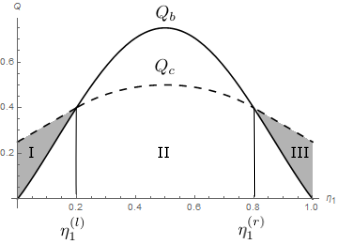
\includegraphics[height=4.5cm]{Fig1.png}}
\protect\caption[\hspace{1cm}$Q_{{\rm c}}$ and $Q_{{\rm b}}$ vs.~$\eta_{1}$]{ $Q_{{\rm c}}$ (dashed line, Eq. (\ref{Qmax})) and $Q_{{\rm b}}$
(solid line, Eq. (\ref{Qb})) vs.~$\eta_{1}$ for $\theta=\pi/3$.
Measurements can be optimized in the area under the dashed line, $Q_{c}$.
Measurements in the area above $Q_{c}$ are suboptimal. In the shaded
areas between $Q_{c}$ and $Q_{b}$ (regions I, left, and III, right)
the optimal FRIO measurement is a projective measurement, in the unshaded
area below $Q_{c}$ (region II) the optimal measurement is a POVM.}
\label{Fig1} 
\end{figure}

%%%%%%%%%%%%%%%%%%%%%%%%%%%%%%%%%%%%%%%%%%%%%%%%
%%%%%%%%%%%%%%%%%%%%%%%%%%%%%%%%%%%%%%%%%%%%%%%%
\section{Interpolative Discrimination}
There are many reasons to consider the problem of allowing both failure and error results in your measurement.
First, experimental implementations are never without error.  Second, success rates may significantly increase for
small changes in the error rate.  This motivates an intermediate strategy
\subsection{Operator Transformation}

We review the original problem in a single two-dimensional Hilbert space, and the solution that  involves a transformation that eliminates the failure operator from the discrimination problem.  We are given two pure states $\rho_1= \ke \psi_1 \br {\psi_1}$ and $\rho_2 = \ke \psi_2 \br{\psi_2}$ with a-priori probabilities $\eta_1$ and $\eta_2$ respectively.  These two probabilities add to one:  $\eta_1 +\eta_2 = 1$. We wish to optimize the success rate  $P_s = \eta_1tr[\Pi_1 \rho_1] + \eta_2 tr[\Pi_2 \rho_2]$ for a fixed failure rate $Q = tr[\Pi_0(\eta_1 \rho_1 + \eta_2 \rho_2)]$ where the measurement operators are the $\Pi_i$ that span the Hilbert space: $\Pi_1 + \Pi_2 + \Pi_0 = I$.  The transformation we implement is
 \begin{equation}
\Omega ^{-1/2}[\Pi_1 + \Pi_2] \Omega^{-1/2} = I,
\end{equation}
where $\Omega = I - \Pi_0$.

Calling the transformed operators $\widetilde \Pi_i$ for $i= 1,2$, we can find the corresponding transformed density matrices $\widetilde \rho_i$ and a-priori probabilities $
\widetilde \eta_i$ to make this a new ME problem that can be readily solved. The minimized error probability as a function of the failure rate is
\begin{equation} P_e = \frac{1}{2} (1 - Q -\sqrt{(1-Q)^2 - (Q-Q_0)^2})\end{equation}
for $Q \leq Q_0 = 2 \sqrt{\eta_1\eta_2} \cos \theta$ where $Q_0$ is the maximum failure rate allowed in the optimization scheme and it corresponds to the best measurement in the UD case.  We will provide an in-depth description of this solution as it pertains to our problem of discriminating mixed states with a Jordan basis structure in the next chapter.



%%%%%%%%%%%%%%%%%%%%%%%%%%%%%%%%%%%%%%%%%%%%%%%%
%%%%%%%%%%%%%%%%%%%%%%%%%%%%%%%%%%%%%%%%%%%%%%%%

\subsection{Neumark Solution of Interpolation}

Since our measurement results must now include the three degrees of freedom from the successful measurements and failure result, in addition to the two degrees of freedom
provided us by the pure states, we require an extra ancillary degree of freedom.  This we add by extending our Hilbert space with a direct sum extension.

\begin{eqnarray}
U \ke {\psi_1}= \sqrt{p_1} \ke 1 + \sqrt{r_1} \ke 2 + \sqrt{q_1} \ke 0 \\
U |\psi_2 \rangle = \sqrt{r_2} \ke 1 + \sqrt{p_2} \ke 2 + \sqrt{q_2} \ke 0 
\end{eqnarray}

Here $p_i$ is the probability that the state i is correctly identified when it is sent into the measurment apparatus, $r_i$ the error rate (mistaking one state for the other) and $q_i$ the failure rate, or not getting a conclusive measurement result.  By sandwiching the preceding equations with their adjoints we confirm that $q_i + r_i+p_i = 1$, the sum of various probabilities is one.

\subsubsection{Equal Weights Solution}

The solution when $\eta_1 = \eta_2=\frac{1}{2}$ is very simple and neat.  Here we have $p_1 = p_2$, $q_1 =q_2$ and $r_1 = r_2$.  Hence $Q = \eta_1 q_1 + \eta_2 q_2 = q_1$

The overlap between the two states $\bk {\psi_2}{\psi_1} = s$ can be also found  by finding the adjoint of one of the Unitary expressions and sandwiching it with the other expression, and since $U U^\dagger = 1$   we find 

\[s = 2 \sqrt{pr} + Q = s \sqrt{p(1-p-q)} + Q\]
Solving for p by squaring we find
\[ (s- Q)^2 = 4p(1-p-q)\] so
\[p^2 -p(1-Q) + (s-Q)^2/4 = 0\] and the positive root gives us the answer as
\[p = \frac{1}{2}[1-Q - \sqrt{(1-Q)^2 -(s-Q)^2}]\]


%%%%%%%%%%%%%%%%%%%%%%%%%%%%%%%%%%%%%%%%%%%%%%%%%%%%%%%%%%%%%%%%%% %%%%%%%%%%%%%%%%%%%%%%%%%%%%%%%%%%%%%%%%%%%%%%%%%%%%%%%%%%%%%%%%%%%%%%%%%%%%%%%%%%%%%%%%%%%%%%%%%%%%%%%%%%%%%%%%%%%%%%%%%%%% 

\subsection{Full Solution}
The total probability of success, error and failure we denote as $P_s = \eta_1 p_1 + \eta_2 p_2$ and $P_r = \eta_1 r_1 + \eta_2 r_2$ and $Q = \eta_1 q_1 + \eta_2 q_2$ respectively.


Taking the inner product

\[s = \langle\psi_1|\psi_2\rangle\ = \sqrt{p_1 r_2} + \sqrt{p_2 r_1} + \sqrt{q_1 q_2}\]

\[= \sqrt{(1-r_1 -q_1 )r_2} + \sqrt{(1-r_2 -q_2 )r_1} + \sqrt{q_1 q_2}\]

This is our overlap constraint.

We now use the Lagrange multiplier method to minimize $P_e$ subject to the overlap constraint.

\[F_e = \eta_1 r_1 + \eta_2 r_2 + \lambda (s - Overlap Constraint )\]

Step one: \[dF/dr_i = 0\]	

 Solve for $r_i (\lambda)$
	
Step two: substitute $s = \sqrt{p_1 r_2} + \sqrt{p_2 r_1} + \sqrt{q_1 q_2}$	
 into $r_i (\lambda)$ and solve for $\lambda$, then plug $\lambda$ into $r_i (\lambda)$.
The details of this calculation are included in Appnedix A.

A lot of algebra gives us the individual error rates as:


\[r_1=\frac{1}{2}[\alpha_1-\frac{[2\eta_2\omega-\alpha_1(1-Q)]}{\sqrt{(1-Q)^2-4\omega\eta_1\eta_2}}]\]


and

\[r_2=\frac{1}{2}[\alpha_2-\frac{[2\eta_1\omega-\alpha_2(1-Q)]}{\sqrt{(1-Q)^2-4\omega\eta_1\eta_2}}]\]


where $\alpha_i \equiv 1-q_i $ and  $\omega\equiv(s -\sqrt{q_1 q_2})^2$

These are not the final result because they were optimized individually. Let us now put these into the expression of minimum error and do a final optimization. First

\[P_E =\eta_1 r_1+\eta_2 r_2\]

\[=\frac{1}{2}[(1-Q)-\sqrt{(1-Q)^2-4\eta_1\eta_2(s-\sqrt{q_1q_2})^2}]\]

We can further minimize this expression since total $Q$ is fixed but we can choose how much of it to place on $q_1$ and $q_2$

To minimize the above expression we can maximize the term under the square root

\[(1-Q)^2-4\eta_1\eta_2(s-\sqrt{q_1q_2})^2\]
\[ = (1-Q)^2-4\eta_1\eta_2(s-\sqrt{\frac{q_1(Q-\eta_1 q_1)}{\eta_2}})^2\]

Since the only part of this expression that is dependent on the variables $q_i$ is the inner square root, we can find an extremum of this part. A simple partial derivative with respect to $q_1$ tells us the optimality condition is $Q = 2 \eta_1 q_1$ or equivalently $\eta_1 q_1 = \eta_2 q_2$

This simplifies our solution to be 


\[P_E=\frac{1}{2}[(1-Q)-\sqrt{(1-Q)^2-(Q-Q_0)^2}]\]


%%%%%%%%%%%%%%%%%%%%%%%%%%%%%%%%%%%%%%%%%%%%%%%%
%%%%%%%%%%%%%%%%%%%%%%%%%%%%%%%%%%%%%%%%%%%%%%%%

%%%%%%%%%%%%%%%%%%%%%%%%%%%%%%%%%%%%%%%%%%%%%%%%
%%%%%%%%%%%%%%%%%%%%%%%%%%%%%%%%%%%%%%%%%%%%%%%%


%%%%%%%%%%%%%%%%%%%%%%%%%%%%%%%%%%%%%%%%%%%%%%%%
%%%%%%%%%%%%%%%%%%%%%%%%%%%%%%%%%%%%%%%%%%%%%%%%
%%%%%%%%%%%%%%%%%%%%%%%%%%%%%%%%%%%%%%%%%%%%%%%%
%%%%%%%%%%%%%%%%%%%%%%%%%%%%%%%%%%%%%%%%%%%%%%%%
\chapter{Discrimination of Mixed States}
\section{Introduction}
Here we consider the problem of discriminating between two mixed states,
\begin{eqnarray}
\rho_1 = \sum_i r_i \vert r_i \rangle \langle r_i \vert, \\
\rho_2 = \sum_i s_i \vert s_i \rangle \langle s_i \vert,
\end{eqnarray}
where their eigenvalues are normalized such that $ \sum_i r_i = \sum_i s_i =1$.  Again we allow for each to occur
with different a-priori probability $\eta_1$ or $\eta_2$ with $\eta_1+\eta_2 =1$.  Since the two states aren't necessarily diagonalizable
in the same basis, the measurement operators must be projectors or POVM's on the joint Hilbert space.  If the two states have non-zero kernels,
then unambiguous discrimination is possible by projecting onto those spaces.  Otherwise we must use a figure of merit such as error or confidence to
optimize our measurement.  We begin with a brief treatment of minimum error discrimination, followed by the solution of the interpolative measurement problem
for several particular mixed states.  We conclude the chapter by describing maximum confidence measurements and a strategy for increasing success rates in high-dimensional measurements via confidence-valued measurement operators. 

%%%%%%%%%%%%%%%%%%%%%%%%%%%%%%%%%%%%%%%%%%%%%%%%
%%%%%%%%%%%%%%%%%%%%%%%%%%%%%%%%%%%%%%%%%%%%%%%%

\subsection{Minimum Error Discrimination}

The first solution was also provided by Helstrom\cite{Helstrom1969}, but we provide an alternative derivation \cite{Fuchs1996,Herzog2004} using
the POVM decomposition of the measurement space.  We consider two detectors $\Pi_1$ and $\Pi_2$ such that $\Pi_1 + \Pi_2 = 1$ with  
$\Pi_1 = \sum_1^d \kb{\lambda_i}{\lambda_i}$, $\Pi_2 = \sum_d^N+1 \kb{\lambda_i}{\lambda_i}$ where the $\ke {\lambda_i}$ form a basis on the total space
of both states of dimension N and is ordered such that the first $d$ vectors are more likely to contain $\rho_1$.

Particularly, the error probability takes the form
\begin{eqnarray}
P_E &=& \frac{1}{2}[ 1 - Tr |\eta_2 \rho_2 - \eta_1 \rho_1|]\\
&=&\frac{1}{2}[ 1 - Tr |\Lambda |]
\end{eqnarray}
Where $\Lambda = \eta_2 \rho_2 - \eta_1 \rho_1$ plays the role of determining the weight of each state in a particular eigenvector.  Its diagonalization gives
\[\Lambda = \sum^N \lambda_i \kb{\lambda_i}{\lambda_i} = \sum_1^d \lambda_{i<0}\kb{\lambda_i}{\lambda_i} + \sum_{d+1}^N\lambda_{i\geq0}\kb{\lambda_i}{\lambda_i}.\]  For eigenvectors belonging
to the value 0, grouping those vectors with either $\Pi_1$ or $\Pi_2$ does not affect the measurement outcomes.  Naturally this equation reduces to the Helstrom
bound for pure states.


%%%%%%%%%%%%%%%%%%%%%%%%%%%%%%%%%%%%%%%%%%%%%%%%
%%%%%%%%%%%%%%%%%%%%%%%%%%%%%%%%%%%%%%%%%%%%%%%%
\section{Mixed States with Jordan Structure}

In this section we discuss the interpolative discrimination of a class of mixed states with a Jordan structure.  As before, 
they are to be discriminated with a-priori probabilities $\eta_1 , \eta_2$ but now their density matricies lie pairwise such
that there are only two vectors per subspace:
\begin{equation}
 \langle r_i \vert s_j \rangle = \delta_{ij} \cos \theta_i
\end{equation}

 In each 2d subspace i there lie an $\vert r_i \rangle$ and  $\vert s_i \rangle$ with a-priori probabilities now
$\eta_{1,i} = \eta_1 r_i$ and $\eta_{2,i} = \eta_2 s_i$.  This structure can be physically interpreted as the transmission of two input states over several fiber optic cables. Each cable contains two degrees of freedom, that could be horizontal and vertical polarization.

The generalization to multiple subspaces is straightforward at first  so we begin with the two subspaces example.

Here our density matrices are in four dimensions that can be described as two tensor product spaces:
\begin{eqnarray}
 \rho_1 &=& r_1 \vert r_1 \rangle \langle r_1 \vert  + r_2 \vert r_2 \rangle \langle r_2 \vert \\
 \rho_2 &=& s_1 \vert s_1 \rangle \langle s_1 \vert  + s_2 \vert s_2 \rangle \langle s_2 \vert. \nonumber\end{eqnarray}
These mixed states are shown in Fig. 1.


Defining our measurement operators for the first subspace as
\begin{equation} \widetilde \Pi_{1,1} + \widetilde \Pi_{2,1} = I_1,\end{equation}
where $I_1$ is the identity matrix of the first subspace.  We define the failure rate for the first subspace as $Q_1 = \xi_1 \ke 0_{11} \br 0 $,which in terms of a measurement probability is also
\begin{equation} Q_1 = \xi_1 [ \eta_{1,1} \cos^2 \phi_1 + \eta_{2,1} \cos^2 (\theta_1 - \phi_1)],\end{equation}
where $\theta_1 $ is the overlap angle between the two states in subspace 1, and $\phi_1$ is the angle $\ke {r_1}$ makes with respect to $\vert 0 \rangle_1$.  The error rate in that subspace is
\begin{equation}P_{e,1} = \eta_{1,1} \langle r_1 \vert \Pi_2 \vert r_1 \rangle + \eta_{2,1} \langle s_1 \vert \Pi_1 \vert s_1 \rangle. \end{equation}
For our simplification trick to work we introduce the normalized state vector \begin{equation} \vert \widetilde{r_1} \rangle  = \frac{ \Omega^{1/2} \vert r_1 \rangle}{\sqrt{\langle r_1 \vert \Omega \vert r_1 \rangle}} \end{equation}
and normalized coefficients
\begin{equation} \widetilde{\eta_{1,1}} = \frac{\eta_{1,1} \langle r_1 \vert \Omega \vert r_1 \rangle}{\eta_{1,1} \langle r_1 \vert \Omega \vert r_1 \rangle + \eta_{2,1} \langle s_1 \vert \Omega \vert s_1 \rangle}\end{equation}
to get 
\[P_{e,1}= \]
\[ [\eta_{1.1} \langle r_1 \vert \Omega \vert r_1 \rangle + \eta_{2,1}\langle s_1 \vert \Omega \vert s_1 \rangle](\widetilde{\eta_{1,1}}\langle\widetilde{r_1} \vert \widetilde{\Pi_2} \vert \widetilde{r_1} \rangle + \widetilde{\eta_{2,1}} \langle \widetilde{s_1} \vert \widetilde{\Pi_1} \vert \widetilde{s_1}\rangle ).\]

We notice that the expression in the ( ) with all tildes contains a pure state minimum error problem, while with the notation $ \eta_{1,1} +\eta_{2,1} = \omega_1$ the left hand set of [ ]  can be reworked into $\omega_1 - Q_1 $ to rewrite the error rate as
\[ P_{e,1}= \frac{1}{2} [\omega_1 - Q_1] (1- \sqrt{1 - 4 \widetilde{\eta_{1,1}} \widetilde{\eta_{2,1}} \vert \langle \widetilde{r_1} \vert \widetilde{s_1} \rangle \vert ^2 }). \]
If we substitute and simplify we find this equals to
\[=\frac{1}{2} ( \omega_1 - Q_1 - \sqrt{ ( \omega_1 - Q_1)^2 -(Q_{0,1} - Q_1 \sin 2 \phi )^2}),\]
where we used the notation $Q_{0,1} = 2 \sqrt{\eta_{1,1}\eta_{2,1}} \cos \theta_1$ and 
 $ \sin \phi = \frac{ \sqrt {\eta_{2,1}} \cos (\theta_1 - \phi_1)}{\sqrt{ \eta_{1,1} \cos^2 (\phi_1)+ \eta_{2,1} \cos^2 (\theta_1 - \phi_1)}}$.  Minimization of the error rate as a function of $\phi_1$ tells us to set $\phi_1 =\frac{\pi}{4}$ so finally
\begin{equation}P_{e,1} = \frac{1}{2} ( \omega_1 - Q_1 - \sqrt{ ( \omega_1 - Q_1)^2 -(Q_{0,1} - Q_1 )^2}).\end{equation}

This result agrees with the single subspace limit and is simply the optimized solution for that subspace alone. We can derive a similar result for the other subspace, so we can consider an optimal distribution of failure among the two subspaces.  However, we want to treat this distribution problem for n subspaces so we first generalize our preceding solution to 2n dimensions.


Recognizing that the likelihood of finding a particle in a subspace isn't 1, we want to normalize our problem so that we can solve it like the 2d case where we had $P_e+ P_s+ Q= 1.$ Instead, in our problem we have $P_{e,i} + P_{s,i} + Q_i = \eta_{1,i} + \eta_{2,i} = \omega_i$ where $P_{s,i}$ and $Q_i$ are the success and the failure probabilities in that subspace.  Since our measurements span the Hilbert space of this subspace, the total probability of a particle being measured therein we call $\omega_i$, or the weight of that subspace.

We can define weighted result probabilities
\begin{equation} \bar{P_{e,i}} +\bar{P_{s,i}} + \bar{Q_i} = 1 \end{equation}
with $ \bar{\bullet} = \frac{\bullet}{\omega_i} $. We can define new constants $\bar{\eta_{1,i}} $ and $ \bar{\eta_{2,i}}$ that still sum 1, so that the states and measurements in (3.8) don't change.  Now it is straightforward to apply the 2d solution to each subspace, where our error rate becomes
\[\bar{P_{e,i}} = \frac{1}{2}( 1-\bar{Q_i} - \sqrt{(1-\bar{Q_i})^2 - (\bar{Q_{0,i}} -\bar{ Q_i})^2}),\]
where $\bar{Q_{0,i}} = 2 \sqrt{\bar{\eta_{1,i}}\bar{\eta_{2,i}}}\cos\theta_i.$
If we remove the bars, this becomes the generaized version of the solution we derived for one subspace in (3.7):
\begin{equation}P_{e,i}= \frac{1}{2}( \omega_i-Q_i - \sqrt{(\omega_i-Q_i)^2 - (Q_{0,i} - Q_i)^2}).\end{equation}




%%%%%%%%%%%%%%%%%%%%%%%%%%%%%%%%%%%%%%%%%%%%%%%%%%%%%%%%%%EX%
%%%%%%%%%%%%%%%%%%%%%%%%%%%%%%%%%%%%%%%%%%%%%%%%%%%%%%%%%%%

\subsection{Subspaces formalism}

To discuss the more general case of higher-dimensional input states we consider a Jordan Basis structure.
Two states are now to be discriminated with a-priori probabilities $\eta_1 , \eta_2$ such that $\rho_1 = \sum r_i \vert r_i \rangle \langle r_i \vert $ and $\rho_2 = \sum s_i \vert s_i \rangle \langle s_i \vert$ with $ \langle r_i \vert s_j \rangle = \delta_{ij} \cos \theta_i$. In each 2d subspace i there lie an $\vert r_i \rangle$ and  $\vert s_i \rangle$ with a-priori probabilities now
$\eta_{1,i} = \eta_1 r_i$ and $\eta_{2,i} = \eta_2 s_i$.  This structure can be physically interpreted as the transmission of two input states over several fiber optic cables. Each cable contains two degrees of freedom, that could be horizontal and vertical polarization.

The generalization to multiple subspaces is straightforward at first  so we begin with the two subspaces example.  


%%%%%%%%%%%%%%%%%%%%%%%%%%%%%%%%%%%%%%%%%%%%%%%%%%%%%%%%%%%%%%%%%%%%%%%%%%%%%%%%%%%%%%%%%%%%%%%%%%%%%%%%%%%%%%%%%%%%%%%%%%%%%%%%  
\subsubsection{Two Subspaces}
Here our density matrices are in four dimensions that can be described as two tensor product spaces:
\begin{eqnarray}
 \rho_1 &=& r_1 \vert r_1 \rangle \langle r_1 \vert  + r_2 \vert r_2 \rangle \langle r_2 \vert \\
 \rho_2 &=& s_1 \vert s_1 \rangle \langle s_1 \vert  + s_2 \vert s_2 \rangle \langle s_2 \vert. \nonumber\\
\end{eqnarray}
%These mixed states are shown in Fig. 1.
%\begin{figure}[th]
%\centering
%$%
%\begin{array}{c}
%\includegraphics[height=4 cm]{Figure1.png} \\
%\end{array}%
%$%
%\caption{Input states in subspaces one and two}
%\label{fig:Graphs}
%\end{figure}

Defining our measurement operators for the first subspace as
\begin{equation} \widetilde \Pi_{1,1} + \widetilde \Pi_{2,1} = I_1,\end{equation}
where $I_1$ is the identity matrix of the first subspace.  We define the failure rate for the first subspace as $Q_1 = \xi_1 \ke 0_{11} \br 0 $,which in terms of a measurement probability is also
\begin{equation} Q_1 = \xi_1 [ \eta_{1,1} \cos^2 \phi_1 + \eta_{2,1} \cos^2 (\theta_1 - \phi_1)],\end{equation}
where $\theta_1 $ is the overlap angle between the two states in subspace 1, and $\phi_1$ is the angle $\ke {r_1}$ makes with respect to $\vert 0 \rangle_1$.  The error rate in that subspace is
\begin{equation}P_{e,1} = \eta_{1,1} \langle r_1 \vert \Pi_2 \vert r_1 \rangle + \eta_{2,1} \langle s_1 \vert \Pi_1 \vert s_1 \rangle. \end{equation}
For our simplification trick to work we introduce the normalized state vector \begin{equation} \vert \widetilde{r_1} \rangle  = \frac{ \Omega^{1/2} \vert r_1 \rangle}{\sqrt{\langle r_1 \vert \Omega \vert r_1 \rangle}} \end{equation}
and normalized coefficients
\begin{equation} \widetilde{\eta_{1,1}} = \frac{\eta_{1,1} \langle r_1 \vert \Omega \vert r_1 \rangle}{\eta_{1,1} \langle r_1 \vert \Omega \vert r_1 \rangle + \eta_{2,1} \langle s_1 \vert \Omega \vert s_1 \rangle}\end{equation}
to get 
\[P_{e,1}= \]
\[ [\eta_{1.1} \langle r_1 \vert \Omega \vert r_1 \rangle + \eta_{2,1}\langle s_1 \vert \Omega \vert s_1 \rangle](\widetilde{\eta_{1,1}}\langle\widetilde{r_1} \vert \widetilde{\Pi_2} \vert \widetilde{r_1} \rangle + \widetilde{\eta_{2,1}} \langle \widetilde{s_1} \vert \widetilde{\Pi_1} \vert \widetilde{s_1}\rangle ).\]

We notice that the expression in the ( ) with all tildes contains a pure state minimum error problem, while with the notation $ \eta_{1,1} +\eta_{2,1} = \omega_1$ the left hand set of [ ]  can be reworked into $\omega_1 - Q_1 $ to rewrite the error rate as
\[ P_{e,1}= \frac{1}{2} [\omega_1 - Q_1] (1- \sqrt{1 - 4 \widetilde{\eta_{1,1}} \widetilde{\eta_{2,1}} \vert \langle \widetilde{r_1} \vert \widetilde{s_1} \rangle \vert ^2 }). \]
If we substitute and simplify we find this equals to
\[=\frac{1}{2} ( \omega_1 - Q_1 - \sqrt{ ( \omega_1 - Q_1)^2 -(Q_{0,1} - Q_1 \sin 2 \phi )^2}),\]
where we used the notation $Q_{0,1} = 2 \sqrt{\eta_{1,1}\eta_{2,1}} \cos \theta_1$ and 
 $ \sin \phi = \frac{ \sqrt {\eta_{2,1}} \cos (\theta_1 - \phi_1)}{\sqrt{ \eta_{1,1} \cos^2 (\phi_1)+ \eta_{2,1} \cos^2 (\theta_1 - \phi_1)}}$.  Minimization of the error rate as a function of $\phi_1$ tells us to set $\phi_1 =\frac{\pi}{4}$ so finally
\begin{equation}P_{e,1} = \frac{1}{2} ( \omega_1 - Q_1 - \sqrt{ ( \omega_1 - Q_1)^2 -(Q_{0,1} - Q_1 )^2}).\end{equation}

This result agrees with the single subspace limit and is simply the optimized solution for that subspace alone. We can derive a similar result for the other subspace, so we can consider an optimal distribution of failure among the two subspaces.  However, we want to treat this distribution problem for n subspaces so we first generalize our preceding solution to 2n dimensions.



%%%%%%%%%%%%%%%%%%%%%%%%%%%%%%%%%%%%%%%%%%%%%%%Generalization %%%%%%%%%%%%%%%%%%%%%%%%%%%%%%%%%%%%%%%%%%%%%%%%%%%%%%%%%%%%%%%%%% %%%%%%%%%%%%%%%%%%%%%%%%%%%%%%%%%%%%%%%%%%%%%%%%%%%%%%%%%%%%%%%%%%%%%%%%%%%%%%%%%%%%%%%%%%%%%%%%%%%%%%%%%%%%%%%%%%%%%%%%%%%% 

\subsubsection{Generalization to n subspaces}

Recognizing that the likelihood of finding a particle in a subspace isn't 1, we want to normalize our problem so that we can solve it like the 2d case where we had $P_e+ P_s+ Q= 1.$ Instead, in our problem we have $P_{e,i} + P_{s,i} + Q_i = \eta_{1,i} + \eta_{2,i} = \omega_i$ where $P_{s,i}$ and $Q_i$ are the success and the failure probabilities in that subspace.  Since our measurements span the Hilbert space of this subspace, the total probability of a particle being measured therein we call $\omega_i$, or the weight of that subspace.

We can define weighted result probabilities
\begin{equation} \bar{P_{e,i}} +\bar{P_{s,i}} + \bar{Q_i} = 1 \end{equation}
with $ \bar{\bullet} = \frac{\bullet}{\omega_i} $. We can define new constants $\bar{\eta_{1,i}} $ and $ \bar{\eta_{2,i}}$ that still sum 1, so that the states and measurements in (3.8) don't change.  Now it is straightforward to apply the 2d solution to each subspace, where our error rate becomes
\[\bar{P_{e,i}} = \frac{1}{2}( 1-\bar{Q_i} - \sqrt{(1-\bar{Q_i})^2 - (\bar{Q_{0,i}} -\bar{ Q_i})^2}),\]
where $\bar{Q_{0,i}} = 2 \sqrt{\bar{\eta_{1,i}}\bar{\eta_{2,i}}}\cos\theta_i.$
If we remove the bars, this becomes the generaized version of the solution we derived for one subspace in (3.7):
\begin{equation}P_{e,i}= \frac{1}{2}( \omega_i-Q_i - \sqrt{(\omega_i-Q_i)^2 - (Q_{0,i} - Q_i)^2}).\end{equation}

%%%%%%%%%%%%%%%%%%%%%%%%%%%%%%%%%%%%%%%%%%%%%%%Lagrangian Optimization PI0%%%%%%%%%%%%%%%%%%%%%%%%%%%%%%%%%%%%%%%%%%%%%%%%%%%%%%%%%%%%%%%%%%%%%
%%%%%%%%%%%%%%%%%%%%%%%%%%%%%%%%%%%%%%%%%%%%%%%%%%%%%%%%%%%%%%%%%%%%%%%%%%%%%%%%%%%%%%%%%%%%%%%%%%%%%%%%%%%%%%%%%%%%%%%%%%%%%%%%%% 
\subsection{Lagrangian Optimization}

Since each subspace failure rate can vary independently we are interested in the optimal values for $Q_i$ as a function of fixed $Q$.
If we consider this a Lagrange Multiplier problem of $P_{e,i}$ and constraint $\sum Q_i = Q$ then we get the constrained function
\begin{equation}F = P_{e,i} - \lambda (\sum Q_i - Q).\end{equation}
We find the minimum of this equation as a function of $Q_i$, substitute into the constraint equation and solve for $\lambda$ to find the optimized value of the individual failure rate as
\begin{equation} Q_i = \frac{Q_{0,i} - \omega_i Q_0 + Q(\omega_i - Q_{0,i})}{1- Q_0}\end{equation}
Now the optimized subspace error rate is
 \begin{equation}P_{e,i}= \frac{1}{2}( \omega_i-Q_i - (\omega_i - Q_{0,i})\sqrt{\frac{1+ Q_0 -2 Q}{1-Q_0}}),\end{equation}
with the total optimal error rate $P_e = \sum P_{e,i}$ is
\begin{equation}P_e = \frac{1}{2}(1-Q-\sqrt{(1-Q)^2-(Q-Q_0)^2}).\end{equation}

We remind ourselves that while this appears identical to the 2d solution (2.2), it in fact contains parameters that are summed over all subspaces.  This means that there is an onto relationship between N dimensional and 2d solutions that allows us to construct a variety of subspace strategies that replicate any 2d solution.
%%%%%%%%%%%%%%%%%%%%%%%%%%%%%%%%%%%%%%%%%%%%%%%%%%%%%%%%%%ThresholdStructure%%%%%%%%%%%%%%%%%%%%%%%%%%%%%%%%%%%%%%%%%%%%%%%%%%%%%%%%%%%%% 
%%%%%%%%%%%%%%%%%%%%%%%%%%%%%%%%%%%%%%%%%%%%%%%%%%%%%%%%%%%%%%%%%%%%%%%%%%%%%%%%%%%%%%%%%%%%%%%%%%%%%%%%%%%%%%%%%%%%%%%%%%%%%%%%  
\subsection{Threshold Structure}

The range of the failure rate solution for subspaces previously derived is valid strictly for more than one subspace and while the upper bound at the UD limit ($Q= Q_0$) is always valid for these equations, the lower bound at the ME solution (Q=0) is not. This limit is restricted by the positivity of $Q_i$:  as we decrease the overall failure rate Q in equation (4.2) we notice that negative solutions are attainable.  Since these are not physical we must prevent $Q_i$ from dropping below 0.  To find the total failure rate at which a subspace's failure rate vanishes we set $Q_i = 0$ in (4.2) to find the critical value of Q for that subspace to be
\begin{equation}Q= Q^i_c = \frac {\omega_i Q_0 - Q_{0,i}}{\omega_i- Q_{0,i}}.\end{equation} 
When Q falls below $Q^j_c$ we fix $Q_j = 0$ and discard that subspace from our optimization.  We realize that after this first threshold we must re-do the optimization with the remaining subspaces. 

It is worthwile to consider also the positivity of the $Q^i_c$, which would make it a real candidate for elimination.  Since $\omega_i - Q_{0,i} \geq 0$ we analyze the positivity of $\omega_i Q_0 - Q_{0,i}$ . For this to be positive we need  $Q_0 \geq \bar{ Q_{0,i}}$ which means that the UD failure rate of that normalized subspace should be smaller than the total UD failure rate of the system of subspaces. 

\subsubsection{First iteration}
 After one subspace failure rate is set to zero, the set of subspaces contributing to the optimization decreases causing changes in the formulas.  To elucidate suppose we order the subspaces such that the highest has the largest $Q^i_c$, and have discarded the $Nth$ subspace associated with $Q_N$ and $\omega_N$ .  This ordering is immutable as will be proven in the subsequent subsection. An analogous optimization over remaining subspaces gives us the failure rates as
\begin{equation}  Q^{(1)}_i = \frac{ Q_{0,i}\Lambda_{N-1}  -  \omega_{i} F_{N-1} + Q( \omega_i - Q_{0,i} ) }{\Lambda_{N-1} - F_{N-1}}\end{equation}
between $Q^N_c \geq Q \geq Q^{(1)N-1}_c$ where we've introduced the notation $\Lambda_k = \sum_1^k \omega_i$ and $F_k = \sum_1^k Q_{0,i}$, and the `1' in parenthesis in $Q^{(1)}_i$ indicates the number of subspaces removed from the Lagrangian optimization.
\subsubsection{General iteration}
We can iterate this process to find the $n$th order failure rates as
\begin{equation}  Q^{(n)}_i = \frac{ Q_{0,i}\Lambda_{N-n}  -  \omega_{i} F_{N-n} + Q( \omega_i - Q_{0,i} ) }{\Lambda_{N-n} - F_{N-n}}.\end{equation}
For every iteration we can also find the nodes of the failure equations, which appear as
\begin{equation}Q^{(n)i}_c = \frac{ \omega_{i} F_{N-n} -  Q_{0,i}\Lambda_{N-n}}{\omega_i - Q_{0,i}}.\end{equation}
This is similar to the first set of critical points found in (5.1). For this to be positive (and to be a candidate for elimination) we need $\frac{ F_{N-n}}{\Lambda_{N-n}} \geq\frac{ Q_{0,i}}{\omega_i}$ which states that the relative UD failure rate for that subspace be smaller than average to be considered for elimination. 

We can derive the ordering for subspaces mentioned earlier from comparing the critical values of two subspaces for a general iteration, and simplify the condition $Q^{(n)i}_c> Q^{(n)j}_c$ to just $\bar{Q_{0,i}}<\bar{Q_{0,j}}$.  Since the second inequality is iteration-independent we can conclude that the subspace with the lowest value of the normalized UD failure rate $\bar{Q_{0,i}}$ will be eliminated first, etc.


%%%%%%%%%%%%%%%%%%%%%%%%%%%%%%%%%%%%%%%%%%%%%%%%%%%%%%%%%%SSD%%%%%%%%%%%%%%%%%%%%%%%%%%%%%%%%%%%%%%%%%%%%%%%%%%%%%%%%%%%%% 
%%%%%%%%%%%%%%%%%%%%%%%%%%%%%%%%%%%%%%%%%%%%%%%%%%%%%%%%%

\subsubsection{Continuity and intersection}

It is worthwile to demonstrate the continuity of our solutions for the $Q_i$'s.  To do this we need to show that the optimal solutions match at the boundaries where a subspace is discarded, or
\begin{equation}Q^{(n)}_i (Q=Q^{(n)N-n}_c) = Q^{(n+1)}_i (Q=Q^{(n)N-n}_c),\end{equation}
where we have chosen to consider the $n$th iteration of the solution and now have decided to discard the $N-n$th subspace.  After we substitute for the expressions for critical points and failure rates, we multiply through by the denominators and group and eliminate like terms we get our desired result.  Continuity allows a physical implementation with variable parameters to smoothly transition from one discrimination regime to the next.

Also interesting is the question of whether the $Q_i$ ever intersect.  We consider this problem in the scope of two subspaces.  If $Q_{0,1} > Q_{0,2}$ and $\frac{d Q_1}{d Q} < \frac{d Q_2}{d Q}$ then the two lines will not cross.  The second condition can be restated in terms of the weights of the subspaces as $\omega_1 < \frac{1+Q_{0,1} - Q_{0,2}}{2}$ or  $\omega_2 > \frac{1+Q_{0,2} - Q_{0,1}}{2}$.  We notice that by our first assumption, the right hand side of the first equation is greater than a half, and smaller than a half in the second equation.  These are sufficient but not necessary conditions. We can also derive the condition for crossing by noting that if $Q_{0,1} > Q_{0,2}$ and $ Q^1_c > Q^2_c$ the lines will intersect.  The second condition can be rewritten as $\bar{Q_{0,1}} < \bar{Q_{0,2}}$, or in terms of the weights as $\omega_1 > \frac{Q_{0,1}}{Q_0}$.
%%%%%%%%%%%%%%%%%%%%%%%%%%%%%%%%%%%%%%%%%%%%%%%%%%%%%%%%%%SSD%%%%%%%%%%%%%%%%%%%%%%%%%%%%%%%%%%%%%%%%%%%%%%%%%%%%%%%%%%%%% 
%%%%%%%%%%%%%%%%%%%%%%%%%%%%%%%%%%%%%%%%%%%%%%%%%%%%%%%%%%%%%%%%%%%%%%%%%%%%%%%%%%%%%%%%%%%%%%%%%%%%%%%%%%%%%%%%%%%%%%%%%%%%%%%%  
\subsection{Single-State Domain}

Each subspace failure rate also has a ceiling.  For the majority of initial conditions the UD failure rate $Q_{0,i}$ sets this upper bound.  For the other cases, we find it from the constraint that $\Pi_{0,i} \leq \vert 0 \rangle_{ii} \langle 0 \vert $.  The equality limit is a full projector which eliminates another measurement and moves us from the POVM to the single-state domain (SSD).

For the single subspace case the equation for the critical ceiling is
\begin{equation} Q = Q_c = \frac{2\eta_1\eta_2 sin^2 \theta}{1-Q_0}.\end{equation}
This result is derived from the constraint that $\xi \leq 1$ where $ \Pi_0 = \xi \vert 0 \rangle \langle 0 \vert$.  Evaluating $\xi$ for the optimal solution gives us $\xi \leq \frac{1-Q_0}{sin^2 \theta} \frac{Q_0}{2 \eta_1 \eta_2}$ where we take the equality limit and set $\xi = 1$ to find the region in which the POVM strategy outperforms the projector measurement. 

There are two regions that this occurs. Assuming $\eta_1 \geq \eta_2$, the SSD overlaps with the interpolation measurement in the region $\frac{1}{1 + \cos^2 \theta} \leq \eta_1$ and when $Q \geq Q_c$.  For $\eta_2 \geq \eta_1$ this happens when $\frac{\cos^2 \theta}{1+\cos^2\theta} \geq \eta_1$ and  $Q \geq Q_c$.  Because the failure operator points directly onto the less likely state in either of these cases, we find the failure rates to be simply $Q^<= \eta_2 + \eta_1 \cos^2 \theta$ and $Q^> = \eta_1 + \eta_2 \cos^2 \theta$ respectively. 

To generalize to subspaces we return to the bar normalization that returned the subspace probabilities to 1.  Remembering that $Q_i =  \xi_i \langle 0_i \vert D_i \vert 0_i \rangle$ where $D_i$ is the full density matrix of the states in the $i$th subspace, $ D_i = \eta_{1,i} \rho_{1,i} + \eta_{2,i} \rho_{2,i}$ we can conclude that $\bar{Q_i} = \xi_i \langle 0_i \vert \bar{D_i} \vert 0_i \rangle$ where $\bar{D_i} = \bar{\eta_{1,i}} \rho_{1,i} + \bar{\eta_{2,i}} \rho_{2,i}$
Now we have restored the summation of the a-priori probabilities for each subspace to 1 while leaving $\xi_i$ unchanged, so the preceding arguments for the single subspace can be implemented to rewrite the inequality for $\xi_i$ as 
\begin{equation} \xi_i \leq \frac{\omega_i-2\sqrt{\eta_{1,i} \eta_{2,i}} \cos \theta_i}{1-\cos^2 \theta_i} \frac{\cos\theta_i}{\sqrt{\eta_{1,i}\eta_{2,i}}}.\nonumber\end{equation} We get the natural generalization of the critical ceiling to subspaces to be
\begin{equation} Q_i = Q^{cc}_i =\frac{2\eta_{1,i} \eta_{2,i} sin^2 \theta_i }{\omega_i-Q_{0,i}}\end{equation} 

As $Q_i$ is increased past this point we have  $\Pi_{1,i} = \vert 1 \rangle_{ii} \langle 1 \vert $ and $\Pi_{0,i} = \vert 0 \rangle_{ii} \langle 0 \vert $. Now the condition for the overlap of the SSD onto the POVM region,  assuming $\eta_{1,i} \geq \eta_{2,i}$ is
 \begin{equation}\frac{\omega_i}{1+\cos^2 \theta_i} \leq \eta_{1,i},\end{equation}
with the maximum failure rate that can be generalized as: $Q^{<}_i = \eta_{2,i} + \eta_{1,i} \cos^2 \theta_i$.
Similarly for $\eta_{2,i} \geq \eta_{1,i}$ we get the condition 
 \begin{equation}\frac{\omega_i \cos^2 \theta_i}{1+\cos^2 \theta_i} \geq \eta_{1,i}\end{equation}
and the maximum failure rate as  $Q^{>}_i = \eta_{2,i} + \eta_{1,i} \cos^2 \theta_i$.


We notice that with more subspaces, the condition for the overlap region of SSD over the POVM does not change for individual subspaces as the bar transformation would show us. We show this structure Fig. 2, where the shaded regions represents the SSD domains.


\bigskip
%%%%%%%%%%%%%%%%%%%%%%%%%%%%%%% SSD graph%%%%%%%%%%%%%%%%%%%%%%%%
%\begin{figure}[th]
%\textbf{$\bar{\eta_{1,i}}$ vs $Q_i$}
%\centering
%$%
%\begin{array}{c}
%\includegraphics[height=4 cm]{Figure2.png} \\
%\end{array}%
%\end{figure}
%$

%\caption{ $\bar\eta_{1,i}$ vs $Q_i$  The dashed line represents $Q_i^{cc}$ and the sold line the absolute maximum $Q_i$, the %intersection point of the two is determined by the inequalities above.  Values given for $\theta_i = \pi /3$ }
%\label{fig:Graphs}
%\end{figure}

%%%%%%%%%%%%%%%%%%%%%%%%%%%%%%%%%%%%%%%%%%%%%%%%%%%%%%%%%%SSD%%%%%%%%%%%%%%%%%%%%%%%%%%%%%%%%%%%%%%%%%%%%%%%%%%%%%%%%%%%%% 
%%%%%%%%%%%%%%%%%%%%%%%%%%%%%%%%%%%%%%%%%%%%%%%%%%%%%%%%%%%%%%%%%%%%%%%%%%%%%%%%%%%%%%%%%%%%%%%%%%%%%%%%%%%%%%%%%%%%%%%%%%%%%%%%  
\subsection{Example}
It is worthwhile to show a numerical example of this method in detail.  We consider three subspaces with $\eta_1 = \eta_2$ and these parameters:
\begin{table}[th] 
%\caption{Nonlinear Model Results} % title of Table 
\centering % used for centering table 
\begin{tabular}{c c c c c c c} % centered columns (4 columns) 
%\hline %inserts double horizontal lines 
Subspace (i)&$r_i$ &$s_i$ &$\theta_i$&$\omega_i$ &$Q_{0,i}$ & $Q_{c,i}$\\ [0.5ex] % inserts table 
%heading 
\hline % inserts single horizontal line 
1 & $\frac{1}{4}$ &$\frac{1}{4}$ &$ \frac{\pi}{4}$ &$\frac{1}{4}$&$\frac{\sqrt{2}}{8}$ & -.39  \\ % inserting body of the table 
2 & $\frac{1}{8}$ &$\frac{3}{8}$  &$\frac{\pi}{6}$ &$\frac{1}{4}$&$\frac{\sqrt{2}}{8}$ & .48\\ 
3 &$\frac{5}{8}$  & $\frac{3}{8}$  &$\frac{\pi}{6}$ &$\frac{1}{2}$&$\frac{\sqrt{2}}{8}$ &-.48  \\  [1ex] % [1ex] adds vertical space 
\hline %inserts single line 
\end{tabular} 
\label{table:example} % is used to refer this table in the text 
\end{table} 

Subspace 1 has its maximum failure rate as $Q_{0,1} = \sqrt{2}/8 \approx .17$. For subspace 2, the maximum failure rate isn't $Q_{0,2} = \sqrt{6}/16 \approx .15$ because it fails one of the SSD conditions and instead $Q^{<}_2 =7/32 \approx .21$, and for subspace 3 the maximum failure rate isn't $Q_{0,3} = 3 \sqrt{5}/16 \approx .42$, because it fails the other SSD condition and instead $Q^{>}_3 = 29/64 \approx .45$. The failure rate maximum $Q^{MAX} = Q_{0,1} +Q^{<}_2 +Q^{>}_3 \approx .87$ while $Q_0 \approx .75$
and $\sum \omega_i = 1$ as it should.

\subsubsection{First elimination}

To find which subspace to discard first we find the critical Q's: $Q^1_c \approx .14$, $Q^2_c \approx .35$, and $Q^3_c <0$, so subspace 2 is discarded first when $Q \approx .35$.  This means that $Q_2 =0$ when $Q = Q^2_c$ and we do not allow the value of $Q_2$ to vary afterward. At $Q^2_c$ we find the values of the other failure rates to be $Q_1 \approx .06$ and $Q_3 \approx .29$

\subsubsection{Second elimination}

It may be clear that $Q_1$ will reach 0 first and indeed this is so.  Before we find the second set of critical values we find our new constants as: $\Lambda_2 = \sum^{1,3}\omega_i = 3/4$; $ F_2 = \sum^{1,3} Q_{0,i} \approx .6$. Now the critical values read $Q^{(1)1}_c \approx .22$ and $Q^{(1)3}_c <0$ so when $ Q = Q^{(1)1}_c$ we discard subspace 1 and reduce the optimization problem to the single subspace case, where $Q^{(2)3} = Q$. This process is depicted in the graph below. 






%%%%%%%%%%%%%%%%%%%%%%%%%%%%%%% Pe1 vs Pe2 and Q1 vs Q2 figures%%%%%%%%%%%%%%%%%%%%%%%%
\iffalse

DO WE NEED THESE GRAPHS? THEY DON'T COME OUT ON THE RIGHT PAGE!!


We include a comparison of the error and failure rates for a different set of initial conditions for two subspaces.

\begin{figure}[b]
\centering
$%
\begin{array}{c}
\includegraphics[height=4 cm]{ParaPe1vsPe2.png} \\ 
\mbox{(a)} \\ 
\begin{array}{c}
\includegraphics[height=4 cm]{ParaQ1vsQ2.png} \\ 
\mbox{(b)} \\ 
\end{array}%
\end{array}%
$%
\caption{Parametrized curve of (a)The error rates for subspace 1 vs subspace 2 as a function of Q (b) $Q_1$ vs $Q_2$ as a function of Q, truncated at $Q_2 = 0$
, both for $\eta_1 = 3/4$ , $r_i = s_i = 1/2$ , $\cos \theta_1 =1/2$, $\cos \theta_2 = \sqrt{3}/2$ and $0 \leq Q \leq 1$}
\label{fig:Graphs}
\end{figure}

\fi
%\FloatBarrier

%%%%%%%%%%%%%%%%%%%%%%%%%%%%%%%%%%%%%%%%%%%%%%%%%%%%%%%%%%%%%%%% 
%%%%%%%%%%%%%%%%%%%%%%%%%%%%%%%%%%%%%%%%%%%%%%%%%%%%%%%%%%%%%%%%%%%%%%%%%%%%%%%%%%%%%%%%%%%%%%%%%%%%%%%%%%%%%%%%%%%%%%%%%%%
\section{Interpolative Mixed Qubit Discrimination} 

Here we discriminate between
\[ \rho_1 = p \ke {\psi_1} \br {\psi_1}  + \frac{(1-p)}{2} I\] 
and
\[ \rho_1 = d \vert \psi_2 \rangle \langle \psi_2 \vert + \frac{(1-d)}{2} I,\]
where the pure states $\vert \psi_1 \rangle = c_1 \vert 0 \rangle + s_1 \vert 1 \rangle $ and $\vert \psi_2 \rangle = c_2 \vert 0 \rangle + s_2 \vert 1 \rangle $ form a 2 dimensional space and p,d are the purities of the two mixed states. We want to implement the same operator transformation as in the previous section.  Since the states are mixed our equations taks the form
\begin{eqnarray}
 \td {\rho_1} &=& \frac{\Omega^{1/2} \rho_1 \Omega^{1/2}}{Tr(\Omega \rho_1)}, \\
\td {\eta_1} &=& \frac{\eta_1 Tr (\Omega \rho_1)}{1-Q},
\end{eqnarray}
so that we still have $Tr \td {\rho_1} = 1 $ and $\td {\eta_1 } + \td {\eta_2} = 1$
and the error rate is$\td{P_e} = \frac{1}{2}(1 - Tr \abs{\td{\Lambda}})$ where $\td{\Lambda} = \td{\eta_1}\td{\rho_1} - \td{\eta_2}\td{\rho_2}$.

Hence 
\[Tr \abs{\td{\Lambda}} = \frac{1}{1-Q} Tr \abs{\Omega^{1/2}\Lambda \Omega^{1/2}}\]
where $\Omega^{1/2} =  \left( \begin{array}{cc}
\sqrt{1- \xi} & 0 \\
0 & 1 \end{array} \right)$ and
$\Lambda = \left( \begin{array}{cc}
{p\eta_1c_1^2-d\eta_2c_2^2 + \frac{\eta_1(1-p) -\eta_2(1-d)}{2}} &{ p\eta_1c_1s_1-d\eta_2c_2s_2} \\
{p\eta_1c_1s_1-d\eta_2c_2s_2} & {p\eta_1s_1^2-d\eta_2s_2^2 + \frac{\eta_1(1-p) -\eta_2(1-d)}{2}}\end{array} \right)$ 
so
$\Omega^{1/2}\Lambda \Omega^{1/2} =$
\[
 \left( \begin{array}{cc}
{(1-\xi)[p\eta_1c_1^2-d\eta_2c_2^2 + \frac{\eta_1(1-p) -\eta_2(1-d)}{2}}] &{\sqrt{1-\xi}( p\eta_1c_1s_1-d\eta_2c_2s_2))} \\
{\sqrt{1-\xi}( p\eta_1c_1s_1-d\eta_2c_2s_2))} & {p\eta_1s_1^2-d\eta_2s_2^2 + \frac{\eta_1(1-p) -\eta_2(1-d)}{2}}\end{array} \right).\]

To find the sum of the absolute values of its eigenvalues we first write the characteristic equation as $ \lambda^2 - b \lambda + c = 0$ where
\[b = \eta_1 -\eta_2 - \xi [ p\eta_1 c_1^2 - d\eta_2 c_2^2 + \frac{\eta_1(1-p) - \eta_2(1-d)}{2}]\]
and
\[c = (1-\xi)[ \frac{1- 4\eta_1\eta_2 -(p\eta_1 -d \eta_2)^2}{4} -pd \eta_1\eta_2 (c_1s_2-c_2s_1)^2].\]
We rewrite the term $ (c_1s_2-c_2s_1)^2 = sin^2 \theta$ and find $\xi$ by solving
\[1-Q = Tr \Omega \rho = 1- \xi [ p\eta_1 c_1^2+ d\eta_2 c_2^2+ \frac{1-p\eta_1 -d\eta_2}{2}]\]
We can solve the quadratic equation $\lambda^2 -b \lambda +c$ for the two eigenvalues, but we notice that for $p=d=1$ the value of c is $c= (1-\xi)[-\eta_1\eta_2 sin^2 \theta]$ is negative and for $p=d=0$ the value of c is $c= (1-\xi)[\frac{(\eta_1-\eta_2)^2}{4}]$ is positive. 

 Hence the sum of the eigenvalues for $c<0$ is
\[\sum \abs {\lambda_i} = \sqrt{b^2-4c}\]
And the sum of the eigenvalues for $c \geq 0$ is
\[\sum \abs {\lambda_i} =b\]

At this point the optimization remains to choose the relationship between the two failure rates, or, equivalently, of $c_1$ and $c_2$.  Since they are constrained by the overlap of the two states, we can easily rewrite this as a function of a single variable and optimize numerically.  However the resulting equation is not tractable algebraically for the general case.  We want to look at the minimum error case for insight into the problem. 

%%%%%%%%%%%%%%%%%%%%%%%%%%%%%%%%%%%%%%%%%%%%%%%%%%%%%%%%%%%%%%%%%%%%%%%%

\subsection{Case: ME limit}
This problem is fairly simple since there is no failure.  We have no need for the transformation and immediately get
%
\[ P_e = \frac{1}{2}(1- Tr \abs \Lambda).\]
Finding the simplified b and c values as
%
\begin{eqnarray*}
b &=& \eta_2 - \eta_1\\
c &=& \frac{1}{4}[ (\eta_1 ^2 - \eta_2^2) - (\eta_1 p - \eta_2 d)^2] - \eta_1 \eta_2 p d sin^2 \theta
\end{eqnarray*}
%
for $c>0$ we get the solution b and for $c<0$ we get the $\sqrt{b^2-4c}$ solution, with no further optimization necessary.  For given initial conditions, positivity doesn't change during the interpolation.

If b is the answer, we find the error rate to be $P_e = \frac{1}{2} (1- (\eta_1-\eta_2)) = \eta_2$ assuming $\eta_1 >\eta_2$.  This strategy is analogous to guessing the more likely state. Otherwise
%
\[P_e = \frac{1}{2}[ 1 - \sqrt{(\eta_1 p +\eta_2 d)^2 - 4\eta_1 \eta_2 p d cos ^2 \theta}]\]
%
which reduces to the Helstrom bound when p=d=1. The critical point c= 0 occurs when 
%
\[ cos^2 \theta = \frac{- (\eta_1 - \eta_2)^2  + (\eta_1 p +\eta_2 d)^2}{4\eta_1 \eta_2 p d}\] 
%%%%%%%%%%%%%%%%%%%%%%%%%%%%%%%%%%%%%%%%%%%%%%%% SUMMARY %%%%%%%%%%%%%%%%%%%%%%%%%%%%%%%%%%%%%%%%%%%%%%%%%%%%%%%%%%%%%%%% 
\section{Maximum Confidence Measurements}
  We begin from the work of Sarah Croke et all 2006 and of Ulrike Herzog, dated from February 2009 on Maximum Confidence.  There two mixed states were measured using 3 POVM's including one failure operator.  The final successful measurement $\Pi_i$ was a normalized, shortened projector onto the eigenket corresponding to the largest eigenvalue of the normalized density matrix $\widetilde{\rho_i}$

Mathematically, given $ \rho_1$ and $\rho_2$, the density matricies of the two states to be distinguished and their a-priori probabilities $\eta_1$ and $\eta_2$, the Maximum Confidence formalism tells us to find:
\[\rho = \eta_1\rho_1 + \eta_2\rho_2\]
 \[ \widetilde{ \rho_i} = \eta_i\rho^{-\frac{1}{2}}\rho_i\rho^{-\frac{1}{2}}\]
\[  \widetilde{ \Pi_i} = \frac{ \rho^{\frac{1}{2}}\Pi_i  \rho^{\frac{1}{2}}}{Tr \rho \Pi_i}   \]
  Where 



\[ C_i = Tr \widetilde{\rho_i} \widetilde{\Pi_i}\] is the $i$th Confidence of the measurement.  The normalized density matrix for the first state is

 \[\widetilde{\rho_1} = v_{max}\vert v_1 \rangle \langle v_{1} \vert + v_{min}\vert v_N \rangle \langle v_N \vert + \sum^{N-1}_{n=2} v_{n}\vert v_n \rangle \langle v_n \vert   \] 
Where we assume that the maximum and minimum eigenvalues are not degenerate.  With the measurement operators taking the form

\[  \Pi_1 = c_1 \rho^{-\frac{1}{2}} \vert v_1 \rangle \langle v_{1} \vert \rho^{-\frac{1}{2}}  \]
\[  \Pi_2 = c_2 \rho^{-\frac{1}{2}}\vert v_N \rangle \langle v_{N} \vert \rho^{-\frac{1}{2}}  \]
\[ \Pi_? = I - \Pi_1 - \Pi_2\]

  Hence we have that the rest of the spectrum of eigenvalues are tossed into the failure operator.  Finally, the probability of failure is minimized while maintaining the rate of Confidence.  

	The new idea is to leave the $ \Pi_1 $ and $ \Pi_2 $, and reduce the failure by a two-fold strategy: First by creating distinct measurements for the remainder of the non-equal eigenvalue spectrum of $\widetilde{\rho_1}$, while assigning the equal eigenvalues to the failure operator.  And second by checking the confidence of the measurement that completes the space, which we distinguish and call the completeness operator.  There would be up to as many distinct operators D+P+2 as $\lambda_{max-(P-1)} \neq 1/2 $ and $ \lambda_{min+(D-1)} \neq 1/2$ for $ D,P < N/2$.  The decreasing difference between the eigenvalues corresponds to decreasing confidence, which can be interpreted as a ladder of confidence-valued POVM's.

 \[\widetilde{\rho_1} = \sum^{D+P}_{\lambda \neq 1/2}\lambda_{i}\vert v_{i} \rangle \langle v_{i} \vert + 1/2\sum^N_{n=D+P+1}\vert v_n \rangle \langle v_n \vert \] 

With the condition that $\lambda_i \geq \lambda_{i+1}$

Our new POVM's would retain two measurements of the previous scheme (those for the extremum eigenvalues) with the additional ones for other eignevalues:


\[  \Pi^{C_1}_1 = c_1 \rho^{-\frac{1}{2}} \vert v_1 \rangle \langle v_{1} \vert \rho^{-\frac{1}{2}}  \]
\[\vdots\]
\[  \Pi^{C_P}_1 = c_P \rho^{-\frac{1}{2}} \vert v_P \rangle \langle v_{P} \vert \rho^{-\frac{1}{2}}  \]
\[  \Pi^{C_{P+1}}_2 = c_{P+1} \rho^{-\frac{1}{2}}\vert v_{P+1} \rangle \langle v_{P+1} \vert \rho^{-\frac{1}{2}}  \]
\[\vdots\]
\[  \Pi^{C_{P+D}}_2 = c_{P+D} \rho^{-\frac{1}{2}}\vert v_{P+D} \rangle \langle v_{P+D} \vert \rho^{-\frac{1}{2}}  \]
\[ \Pi^{\frac{1}{2}} =  c_{P+D} \rho^{-\frac{1}{2}}\sum^N_{n=D+P+1}\vert v_n \rangle \langle v_n \vert \rho^{-\frac{1}{2}} \]
\[\Pi_? = I -\sum^{P}_{i=1} \Pi^{C_i}_1 - \sum^{D}_{i=1} \Pi^{C_{P+i}}_2  - \Pi^{\frac{1}{2}}\]

Where the last two are the new failure and completeness operators.  We distinguish the two because the completeness operator may serve as a measurement in specific schemes.  Before we explore the $\Pi_?$ measurement let's note that the probability of successful measurement so far will be \[P_s = \eta_1 Tr \rho_1 \sum^{P}_{n=1}c_{n} \Pi^{C_n}_1 +  \eta_2 Tr \rho_2 \sum^{D}_{n=1}c_{P+n} \Pi^{C_{P+n}}_2\]

  The failure operator $\Pi^{\frac{1}{2}}$ is hence only neccessary for the range of the spectrum in which both states are equally likely, and the new ? measurement that completes the space we can optimize after we decide the main measurement strategy.

To demonstrate the strategy let us first consider several simplified examples.

Discrimination between two mixed states in 3 dimensions with 1 dimensional kernels.  In this situation we can reinterpret $\Pi_?$.  Suppose 
\[ \rho_1 = \frac{5}{9}(\vert v_1 \rangle \langle v_1 \vert + \frac{4}{5} \vert v_2 \rangle \langle v_2 \vert)\] and
\[ \rho_2 = \frac{5}{6}(\vert v_3 \rangle \langle v_3 \vert + \frac{1}{5} \vert v_2 \rangle \langle v_2 \vert)\]

with equal a-priori probabilities $\eta_1 = \eta_2$

now we solve the problem for maximum confidence measurements:

\[ \rho = \eta_1 \rho_1 + \eta_2 \rho_2 = \frac{1}{36}(10 \vert v_1 \rangle \langle v_1 \vert + 11 \vert v_2 \rangle \langle v_2 \vert + 15 \vert v_3 \rangle \langle v_3 \vert)
 \]

\[ \rho^{1/2} = \frac{1}{6}( \sqrt{10} \vert v_1 \rangle \langle v_1 \vert + \sqrt{11} \vert v_2 \rangle \langle v_2 \vert + \sqrt{15} \vert v_3 \rangle \langle v_3 \vert)
\]

\[ \rho^{-1/2} = 6( \frac{1}{ \sqrt{10}} \vert v_1 \rangle \langle v_1 \vert + \frac{1}{\sqrt{11}} \vert v_2 \rangle \langle v_2 \vert + \frac{1}{\sqrt{15}} \vert v_3 \rangle \langle v_3 \vert)
\]

\[ \widetilde{\rho_1} =( \vert v_1 \rangle \langle v_1 \vert +\frac{8}{11} \vert v_2 \rangle \langle v_2 \vert)
\]

\[ \widetilde{\rho_2} =( \vert v_3 \rangle \langle v_3 \vert +\frac{3}{11} \vert v_2 \rangle \langle v_2 \vert)
\]
Clearly, the measurements take the form
\[\Pi_1 = \vert v_1 \rangle \langle v_1 \vert \]
\[ \Pi_2 = \vert v_3 \rangle \langle v_3 \vert \]
\[ \Pi_? = \vert v_2 \rangle \langle v_2 \vert \]

and $C_1 = C_2 = 1$ implies unambiguous discrimination.
Thus we attain the success probability of the measurement as

\[ P_s = \eta_1 Tr(\rho_1 \Pi_1) + \eta_2 Tr(\rho_2 \Pi_2) = \frac{1}{2}(\frac{5}{9} + \frac{5}{6}) = \frac{25}{36}\]

with failure probability equalling the difference from unity,

\[ Q = 1-P_s = \frac{11}{36}\]

Since the middle eigenvalue isn't $\frac{1}{2}$, if we assign Confidence-Valued POVM's to each eigenvalue we get:

\[\Pi_1 = \vert v_1 \rangle \langle v_1 \vert \]
\[ \Pi^{\frac{8}{11}}_1 = \vert v_2 \rangle \langle v_2 \vert \]
\[ \Pi_2 = \vert v_3 \rangle \langle v_3 \vert \]


We have no failure operator and thus have $Q=0$, instead creating a success probability associated only with the measurement along $\vert v_2 \rangle $

\[ P'_s = \eta_1 Tr( \rho_1 \Pi^{\frac{8}{11}}_1 )= \frac{1}{2}(\frac{4}{9})=\frac{8}{36}\]

and again $C_1 = C_3 = 1$ for the projectors onto the kernels while $C_2 = \frac{8}{11}$ is the confidence of the newly-interpreted measurement.

so that the total success of the new measurement strategy is:

\[P^{tot}_s = P_s + P'_s = \frac{33}{36}\]

Our strategy has lost none of the advantages of unambiguous discrimination and has significantly improved the probaility of success.  By allowing for more than a single measurement to detect one particle, we have a meaningful strategy for handling higher-dimensional discrimination problems:

For two states in 7 dimensions with equal prior probabilities, suppose the density matricies are

\[ \rho_1 = \frac{2}{7}(\vert v_1 \rangle \langle v_1 \vert +  \frac{4}{5} \vert v_2 \rangle \langle v_2 \vert +  \frac{4}{5} \vert v_3 \rangle \langle v_3 \vert +  \frac{1}{2} \vert v_4 \rangle \langle v_4 \vert+  \frac{1}{5} \vert v_5 \rangle \langle v_5 \vert +  \frac{1}{5} \vert v_6 \rangle \langle v_6 \vert )
\] and
\[ \rho_2 = \frac{2}{7} ( \vert v_7 \rangle \langle v_7 \vert + \frac{1}{5} \vert v_2 \rangle \langle v_2 \vert +  \frac{1}{5} \vert v_3 \rangle \langle v_3 \vert +  \frac{1}{2} \vert v_4 \rangle \langle v_4 \vert+  \frac{4}{5} \vert v_5 \rangle \langle v_5 \vert +  \frac{4}{5} \vert v_6 \rangle \langle v_6 \vert )
\]

Following our strategy we write:

\[\rho = \frac{1}{7} I_7\]
\[\rho^{\frac{1}{2}} = \frac{1}{\sqrt{7}}I_7\]
\[\rho^{-\frac{1}{2}} = \sqrt{7}I_7\]

\[ \Pi_1 = \vert v_1 \rangle \langle v_1 \vert\]
\[ \Pi^{\frac{4}{5}}_1 = \vert v_2 \rangle \langle v_2 \vert\]
\[ \Pi^{\frac{4}{5}}_1 = \vert v_3 \rangle \langle v_3 \vert\]
\[ \Pi^{\frac{1}{2}} = \vert v_4 \rangle \langle v_4 \vert\]
\[ \Pi^{\frac{4}{5}}_2 = \vert v_5 \rangle \langle v_5 \vert\]
\[ \Pi^{\frac{4}{5}}_2 = \vert v_6 \rangle \langle v_6 \vert\]
\[ \Pi_2 = \vert v_7 \rangle \langle v_7 \vert\]

\[ P_s = \eta_1 Tr(\rho_1 \Pi_1) + \eta_2 Tr(\rho_2 \Pi_2) = \frac {10}{35} \]
 is the success probability of the UD measurements and $ Q = \frac{25}{35}$
\[ P'_s = \eta_1 Tr(\rho_1 \Pi^{\frac{4}{5}}_1) + \eta_2 Tr(\rho_2 \Pi^{\frac{4}{5}}_2) =  \frac{16}{35}  \]
is the success probability of the ME measurements
\[P^{tot}_s = P_s + P'_s = \frac{26}{35}\]
\[P'_{err} = \frac{4}{35}\]
\[Q' = \frac{5}{35}\]

Now we apply the theory to existing situations, beginning with the simplest, two symmetric pure states in 2d:



First we show the example of an attempt to improve the success probability for IDP measurements.
\[ \vert \psi_1 \rangle = cos \theta \vert 0 \rangle + sin \theta \vert 1 \rangle \]
\[ \vert \psi_2 \rangle = cos \theta \vert 0 \rangle - sin \theta \vert 1 \rangle \]
\[\rho_i = \vert \psi_i \rangle \langle \psi_i \vert\]
The well known measurements take the form

\[ \Pi_1 = a_1 \vert \phi_1 \rangle \langle \phi_1 \vert \]
\[ \Pi_2 = a_2\vert \phi_2 \rangle \langle \phi_2 \vert \]
\[ \Pi_? = 1-\Pi_1 - \Pi_2\]
where
\[ \vert \phi_1 \rangle = sin\theta \vert 0 \rangle + cos\theta \vert 1 \rangle\]
\[ \vert \phi_1 \rangle = sin\theta \vert 0 \rangle - cos\theta \vert 1 \rangle\]

and 

\[ a_1  = \frac{1-\sqrt{\frac{\eta_2}{\eta_1}}cos2\theta}{sin^2 2\theta}\]
\[ a_2  = \frac{1-\sqrt{\frac{\eta_1}{\eta_2}}cos2\theta}{sin^2 2\theta}\]

for unequal a-priori probabilities

Now
\[P_s = \eta_1 Tr \rho_1 \Pi_1 + \eta_2 Tr \rho_2 \Pi_2 = 1-2\sqrt{\eta_1 \eta_2}cos2\theta\]
\[Q = 2\sqrt{\eta_1 \eta_2} cos2\theta\]

Interestingly, even when \[ \eta_1 > \eta_2 \] the failure operator clicks equally often for both states.
\[q_1 = \eta_1 Tr \rho_1 \Pi_0 = \eta_1 (  Tr \rho1 - Tr \rho_1 \Pi_1 - Tr \rho_1 \Pi_2 ) = \eta_1 (1 - 4 a_1 cos^2 \theta sin^2 \theta) = \sqrt{\eta_1 \eta_2} cos 2 \theta \]
So if we associate it with a measurement for the first state we only muddle the success and error probabilities.

This result suggests than an improvement  can be attained with two pure states in 2 dimensions in which the failure rate for each state is different.

We consider the formalism of Bagan:

\[ \Pi_0 = \xi \vert 0 \rangle \langle 0 \vert \]


\[ \vert \psi_i \rangle = c_i\vert 0 \rangle + s_i \vert 1 \rangle \]

\[q_1 = \eta_1 Tr \Pi_0 \rho_1 = \eta_1 \xi c_1^2 \] and 
 \[q_2 = \eta_1 Tr \Pi_0 \rho_2 = \eta_2 \xi c_2^2 \]  are the failure rates for each state

For the case when the failure rates differ,


\[\frac{\eta_1 c_1^2 }{   \eta_2 c_2^2 }>1\] is the condition for which the failure operator clicks more often for the first state than the second, and can be used to describe an additional measurement.

For the case of 2 mixed states in two dimensions:

\[ \rho_ i =
\frac{1}{2} \left( { \begin{array}{cc}
1+r_i cos 2 \theta_i & r_i sin 2 \theta_i\\
 r_i sin 2 \theta_i & 1+r_i cos 2 \theta_i  \\
\end{array} } \right)
\]

\[\eta_1 = \eta_2\]

\[q_1 = \eta_1 Tr \Pi_0 \rho_1 =\frac{1}{4} \xi ( 1+r_1 cos 2 \theta_1 )\] and 
 \[q_2 = \eta_2 Tr \Pi_0 \rho_2 = \frac{1}{4} \xi (1+r_2 cos 2 \theta_2) \]  are the failure rates for each state

so for a reassignment of the failure operator to make sense, the condition \[q_1 > q_2\] or

\[r_1 cos 2 \theta_1 > r_2 cos 2 \theta_2\] must hold

giving us new success and failure probabilities 

\[P'_s = q_1\]
\[P'_e = q_2\]
\[Q'=0\]
so perhaps we need to consider asking a different optimization question for this case, since fixing Q makes no statement about the relation of its contents. 

Let's consider the confidence associated with state one and $\Pi_?$ in two dimensions.

\[ C_? = \frac{\eta_1 Tr \rho_1 \Pi_0}{Tr \rho \Pi_0} = \frac {q_1}{q_1 + q_2} \]

\[ q_1 = \eta_1 Tr \rho_1 \Pi_? = \eta_1 ( 1 - Tr[ \rho_1( \Pi_1 + \Pi_2) ])\]
\[ q_2 = \eta_2 Tr \rho_2 \Pi_? = \eta_2 ( 1 - Tr[ \rho_2( \Pi_1 + \Pi_2) ])\]

The condition for $q_1 > q_2$ is 

\[ \eta_1 - \eta_2  > Tr ( \Pi_1 + \Pi_2) (\eta_1 \rho_1 - \eta_2 \rho_2 ) \] 

In the Maximum Confidence framework this is
\[ \eta_1 - \eta_2  > Tr \rho^{-1} ( \alpha_1 \widetilde{ \Pi_1} + \alpha_2 \widetilde{ \Pi_2 }) (\eta_1 \rho_1 - \eta_2 \rho_2 )\]


Finally we look at the last example offered in Herzog's Max Conf. with minimum failure paper for a case with higher-dimensional operators:
2 mixed states in d dimensions, d even, with equal a-priori probabilities.

\[ \rho_i = \frac{2p}{d} \sum^{d/2}_{k=1} \vert r^{(i)}_k \rangle \langle r^{(i)}_k \vert + (1-p)\frac{I_d}{d}\]
where \[ \vert r^{(i)}_k \rangle = c_k \vert 0 \rangle \pm s_k \vert 1 \rangle \]

Herzog provides us with the MaxConf operators

\[\Pi^{MC}_1 =  \sum^m_{k=1} \frac{ \vert v^{\gamma_{max}}_k \rangle \langle v^{\gamma_{max}}_k \vert }{1+p cos \gamma^{max}}\]
\[\Pi^{MC}_2 =  \sum^m_{k=1} \frac{ \vert w^{\gamma_{max}}_k \rangle \langle w^{\gamma_{max}}_k \vert }{1+p cos \gamma^{max}}\]
where
\[ \vert v^{(\gamma_k)}_k / w^{(\gamma_k)}_k \rangle = \sqrt{\frac{1-p cos \gamma_k}{2}}\vert 0 \rangle_k \pm \sqrt{\frac{1+p cos \gamma_k}{2}}\vert 1 \rangle_k \]
with failure rate \[Q^{MC} = 1-\frac{2m}{d}p cos \gamma^{max} \]
and confidences 
\[ C_1 = C_2 = \frac{1}{2} + \frac{p sin \gamma_{max} }{2 \sqrt{1-p^2 cos^2 \gamma_k}}\]
She also mentions that an alternative, average,  measurement where all the dimensions contribute to conclusive results can be implemented:

\[\Pi^{avg}_1 =  \sum^{d/2}_{k=1} \frac{ \vert v^{\gamma_{k}}_k \rangle \langle v^{\gamma_{k}}_k \vert }{1+p cos \gamma^{k}}\]
\[\Pi^{avg}_2 =  \sum^{d/2}_{k=1} \frac{ \vert w^{\gamma_{k}}_k \rangle \langle w^{\gamma_{k}}_k \vert }{1+p cos \gamma^{k}}\]
with failure rate \[Q^{avg} = \frac{2p}{d} \sum^{d/2}_1 cos \gamma^{k} \]
and necessarily smaller confidences
\[C^{avg}_1 = C^{avg}_2 = \frac{1}{2} + \frac{p \sum^{d/2}_{k=1} sin \gamma_k \sqrt{\frac{1-p cos\gamma_k}{1+p cos \gamma_k}}}{2 \sum^{d/2}_{k=1} (1-p cos \gamma_k)}\]

Now following our new strategy of multiple measurement operators for each state:
\[\Pi^{C_j}_1 =  \sum^{m_j}_{k=1} \frac{ \vert v^{\gamma_{k}}_k \rangle \langle v^{\gamma_{k}}_k \vert }{1+p cos \gamma^{k}}\]
\[\Pi^{C_j}_2 =  \sum^{m_j}_{k=1} \frac{ \vert w^{\gamma_{k}}_k \rangle \langle w^{\gamma_{k}}_k \vert }{1+p cos \gamma^{k}}\]


where $m_i$ denotes the size of the degenerate space associated with $\gamma_i$

with failure rate \[Q = Q^{avg} = \frac{2p}{d} \sum^{d/2}_1 cos \gamma^{k} \]
and confidences 
\[ C_j = \frac{1}{2} + \frac{p sin \gamma^{j} }{2 \sqrt{1-p^2 cos^2 \gamma^j}}\]

Clearly 
\[ \sum^{d/2}_{i=1} \Pi^{C_i}_k= \Pi^{avg}_k\]
So we've found an effective intermediate strategy that maximizes simultaneously the confidence and success of the measurement by utilizing more results for each state.

We have also opened the door for more optimization searches.  For example, the solution set to the 2 states in 2d problem for which $q_1 > q_2$ implies three operators ${\Pi_1,\Pi'_1,\Pi_2}$ will achieve higher rates of success than nearby equal-failure solutions, and so begs for an optimization condition on the competing values of total confidence and success in a measurement.

As for the experimental implementation of multiple measurements for each state we may borrow from Croke's explanation of the additional measurement for failure: The first measurement has associated outcomes $\lambda_{fail}$ and $\lambda_{success}$ and associated POM elements $\Pi_{succ}$ and $\Pi_{fail}$ where a successful measurement transforms the states $\rho_1$ and $\rho_2$ into $\widetilde{\rho_1}$ and  $\widetilde{\rho_2}$ which are then discriminated by $\widetilde{\Pi_1}$ and $\widetilde{\Pi_2}$

There should be a distinction between the equal confidence operator and the operator the completes the space. For non-orthogonal strategies there is an operator the completes the space.  
Call it $\Pi_\frac{1}{2}$ and $ \Pi_?$ clearly for 2d intermediate strategies the way to minimize an operator is to make it symmetric

The first thing should be to do, is to check its confidence.  So there's the failure operator, and the completeness operator.  Now for the completeness operator to distinguish both states equally likely is the condition that projects the states into $\widetilde{\rho_i}$ and allows measurement by $\widetilde{\Pi_i}$

%%%%%%%%%%%%%%%%%%%%%%%%%%%%%%%%%%%%%%%%%%%%%%%%%%%%%%%%%%%%%%%%%%%%%%%%%%%%%%%%%%%%%%%%%%%%%%%%%%%%%%%%%%%%%%%%%%%%%%%%%%%

  
%%%%%%%%%%%%%%%%%%%%%%%%%%%%%%%%%%%%%%%%%%%%%%%%
%%%%%%%%%%%%%%%%%%%%%%%%%%%%%%%%%%%%%%%%%%%%%%%%
%%%%%%%%%%%%%%%%%%%%%%%%%%%%%%%%%%%%%%%%%%%%%%%%
%%%%%%%%%%%%%%%%%%%%%%%%%%%%%%%%%%%%%%%%%%%%%%%%
\chapter{Cloning Pure States}

 The interest of quantum systems comes from their intrinsically probabilistic nature. If perfect cloning of quantum states were possible, this uncertainty would vanish, thus providing an intuitive argument for why perfect cloning is not determinstically feasible.  There have been two different strategies for dealing with the problem of cloning states:  one is to always produce clones that are 'as close' to the originals as possible, usually by means of global fidelity, as was first done for arbitrary states(\cite{Hillery and Buzek 22}) and then for one of two known pure states ( Bennett, etc).  

The other stategy is to sometimes make perfect copies, at the cost of sometimes failing to do so.  The seminal paper by Duan and Guo (cite Duan Guo) solved the problem of making perfect clones probabilistically for equal a-priori conditions, and set this success probability as an upper bound for general a-priori probabilities. While other work has improved on this bound ( ), there has until now been no general solution.  Other perfect probabilistic cloning schemes focus on other types of states ().

 Work has also been done on intermediate strategies where fidelity is maximized for a certain rate of failure, either pure states (cite Chefles) or mixed (Fiurasek, Setaski). There are practical reasons for wanting to produce perfect clones (cite applications), with applications in communication and computing. Experiments have been suggested (cite Fiurasek) and implemented (cite Muller) for cloning quantum states.

Finally, there is a deep relationship between cloning and state discrimination, where the asymptotic behavior of cloning strategies has been shown to reproduce known measurement results (cite Bae, Bennett). More information may be found in a review (cite review)

In this chapter we discuss the transformation which takes an input state and ancilla together to make extra
versions of the input state.  The conversation began with a paper on superluminal communication \cite{who?}
by making copies of quantum states. This was soundly refuted by \cite{Wooters and Zurek 19, Dieks 20} who gave proofs
of the no-cloning theorem for quantum states.  We include a simple version here:

\subsection{No-Cloning Theorem}
Suppose we wrote the equations describing the unitary that cloned one of two known input pure states $\psi_i$ with
a-priori probabilities $\eta_i$ for $i = 1,2$.  If we could perform this measurement perfectly we would write
\begin{eqnarray}
U\ke{\psi_1}\ke 0 = \ke{\psi_1}\ke{\psi_1}\\
U\ke{\psi_2}\ke 0 = \ke{\psi_2}\ke{\psi_2}
\end{eqnarray}
However, taking the inner product of the two equations we find $\bk{\psi_1}{\psi_2} = \bk{\psi_1}{\psi_2}^2$,
restricting the functionality of this unitary to the trivial case when the two states are orthogonal and $\bk{\psi_1}{\psi_2}=0$.
Therefore there does not exist in general a unitary to perform this ideal cloning task.  As with state discrimination, 
we must choose a figure of merit to maximize for given initial conditions.

%%%%%%%%%%%%%%%%%%%%%%%%%%%%%%%%%%%%%%%%%%%%%%%%
%%%%%%%%%%%%%%%%%%%%%%%%%%%%%%%%%%%%%%%%%%%%%%%%se
\section{Deterministic Approximate Cloning}

In this section we derive the 'minimum error' cloning method and make two imperfect copies of one of two input states.  The input states are$\ke{\psi_1} = \cos \theta \ke 0 + \sin \theta \ke 1$,$ \ke{\psi_2} = \cos \theta \ke 0 - \sin \theta \ke 1 $,and the output states are
\[ \ke{\phi_1} = \cos \phi_1 \ke 0 + \sin \phi_1 \ke 1,\]
\[ \ke{\phi_2} = \cos \phi_2 \ke 0 - \sin \phi_2 \ke 1.\]
The unitary representation of this transformation is
\[U \ke{\psi_1} = \ke {\phi_1}\ke{\phi_1},\]
\[U \ke{\psi_2} = \ke {\phi_2}\ke{\phi_2}.\]
The function we want to maximize is the average fidelity
\[F = \eta_1 \bk{\psi_1}{\phi_1}^2 +\eta_2 \bk{\psi_1}{\phi_1}^2\]
The Lagrange multiplier method isn't necessary here as we can rephrase the problem in just one variable. First we rewrite the fidelity by noticing $\bk{\psi_1}{\phi_1} = \cos (\theta - \phi-1) = \cos ( \theta - \frac{\phi_1 + \phi_2}{2} - \frac{\phi_1 - \phi_2}{2}) = \cos ( \alpha - x)$.  Similarly $\bk{\psi_2}{\phi_2} = \cos(\theta - \phi_2) = \cos( \alpha + x)$ so that
\[F = \eta_1 \cos^2( \alpha-x) + \eta_2 cos^2(\alpha + x)\]
is just a function of x.  Differentiating to find the minimum we find the optimal relation between alpha and x as
\[\tan 2x = (\eta_1 - \eta_2) \tan 2 \alpha\]
To make use of this relation we can rewrite the fidelity as
\[F = \eta_1( \cos (2(\alpha - x))+1)/2 + \eta_2(\cos(2(\alpha + x))+1)/2 =\]
\[ \frac{1}{2}[\cos 2\alpha \cos 2x( 1 +(\eta_1 -\eta_2) \tan 2 \alpha\tan 2x)] + \frac{1}{2}.\]
And we can rewrite\[\cos 2 x = \frac{1}{\sqrt{1 + (\eta_1 - \eta_2)^2 \tan^2 2 \alpha}}\] to eliminate x to write 
\[F = \frac{1}{2}( \cos 2 \alpha \sqrt{1 + (\eta_1 - \eta_2)^2 \tan^2 2 \alpha}) + \frac{1}{2}.\]
Inserting the $\cos$ term into the square root we find
\[\cos^2 2 \alpha  + (\eta_1 - \eta_2)^2 \sin^2 2\alpha =  \cos^2 2 \alpha  + (\eta_1 + \eta_2)^2 \sin^2 2\alpha - 4 \eta_1 \eta_2 \sin^2 2 \alpha = 1 - 4 \eta_1 \eta_2 \sin^2 2\alpha,\]
leaving us with the fidelity in its final form as
\[F = \frac{1}{2}( 1 + \sqrt{1-  4 \eta_1 \eta_2 \sin^2 2\alpha}).\]


%%%%%%%%%%%%%%%%%%%%%%%%%%%%%%%%%%%%%%%%%%%%%%%%
%%%%%%%%%%%%%%%%%%%%%%%%%%%%%%%%%%%%%%%%%%%%%%%%
%%%%%%%%%%%%%%%%%%%%%%%%%%%%%%%%%%%%%%%%%%%%%%%%
%%%%%%%%%%%%%%%%%%%%%%%%%%%%%%%%%%%%%%%%%%%%%%%%
\section{Probabilistic Exact Cloning}


We envision a state dependent probabilistic cloner as a machine with an input port, an output port and two flags that herald the success or failure of cloning.  The input $|\psi_i^m\rangle=|\psi_i\rangle^{\otimes m}$, $i=1,2$ ($m$ identical copies of either $|\psi_1\rangle$ or $|\psi_2\rangle$) is fed through the input port for processing. In case of success, $n$ perfect clones~$|\psi_i^n\rangle=|\psi_i\rangle^{\otimes n}$ are delivered through the output port with probability $p_i$, conditioned on the input state being $|\psi^m_i\rangle$. Otherwise, the output is in a generic failure state, with a failure probability~$q_i=1-p_i$.

For cloning, optimality is usually addressed from a Bayesian viewpoint that assumes the states to be cloned are prepared with some prior probabilities $\eta_1$ and $\eta_2$, $\eta_1+\eta_2=1$. Then a natural cost function for the probabilistic cloning machine is the average failure probability, 
%
\begin{equation}
Q=\eta_1 q_1+\eta_2 q_2.
\label{obj fun}
\end{equation}
%
The aim is to find the optimal cloner that minimizes the cost function $Q$, and yields the minimum average failure probability $Q_{\rm min}$ for arbitrary priors $\eta_1$ and $\eta_2$.

In our formulation, similar to that in~\cite{DuanGuo}, the Hilbert space ${\mathscr H}^{\otimes m}$ of the original $m$ copies is supplemented by an ancillary space~${\mathscr H}^{\otimes(n-m)}\otimes {\mathscr H}_F$ that accommodates the additional $n-m$ clones and the success/failure flags. Next, we introduce a unitary transformation~$U$ via
%
\begin{equation}
U|\psi^m_i\rangle|0\rangle= \sqrt{p_i}|\psi^n_i\rangle\ke 1 +\sqrt q_i \rangle \ke 0,\quad i=1,2. \label{Ui}
\end{equation}
%
Here the ancillas are initialized in a reference state~$\ke 0$. The states of the flag associated with successful cloning, $\ke 1$, is orthogonal to the state associated with failure, $\ke {0}$.  While this treatment is standard in the literature \cite{DuanGuo, review}, we will justify it and explore its boundaries subsequently.  At
this stage of complexity the problems we are formulating may have several interpretations.  In our case, for example, we will want to rule out such options as 
orthogonal measurement results for successful cloning, since this will also discriminate the states.  For now we accept it as correct.

To proceed, we take the inner product of equation~$i$ with itself in \eqref{Ui}, yielding that the probabilities are normalized, $p_i+q_i=1$. Taking the inner product of equation $i=1$ with $i=2$ in \eqref{Ui} yields the main constraint, 
%
\begin{equation}
s^m=\sqrt{p_1 p_2}\, s^n+\sqrt{q_1 q_2},
\label{unit cond}
\end{equation}
%
which is a consequence of the unitarity of $U$. Here we  used the notation $s \equiv \bk {\psi_1}{\psi_2}$. 
%%%%%%%%%%%%%%%%%%%%%%%%%%%%%%%%%%%%%%%%%%%%%%%%
%%%%%%%%%%%%%%%%%%%%%%%%%%%%%%%%%%%%%%%%%%%%%%%%
\subsection{Geometric description of optimality}



Before developing the analytical theory of optimizing (minimizing) $Q$, we present a geometric picture, similar in spirit to that in~\cite{Bergou1}, that visually solves the optimization problem and serves as guide for the subsequent calculations. 
\begin{figure}[h,t]
\centering
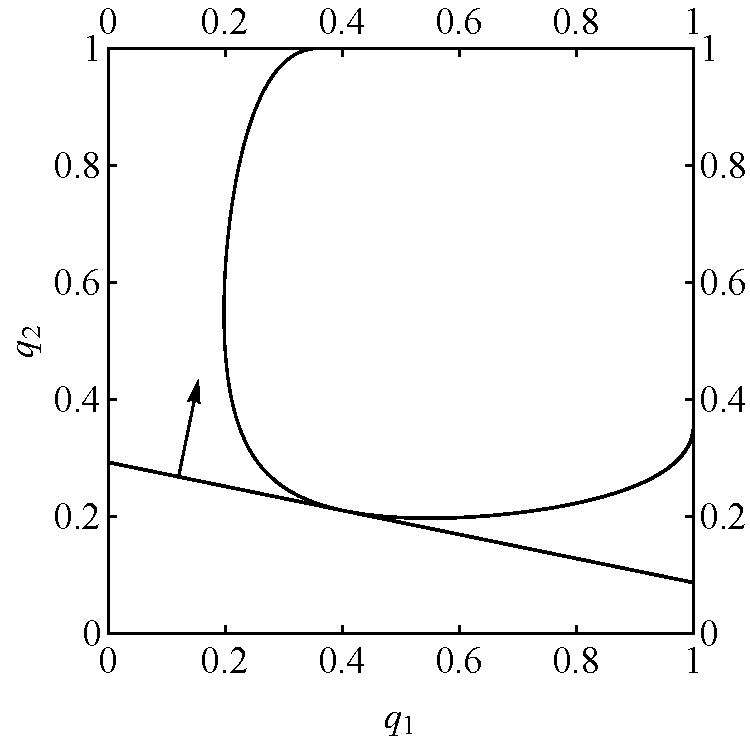
\includegraphics[width=14em]{Figures_CLONEvedit.pdf}
%
\caption{Unitarity curve, $q_{2}$ vs. $q_{1}$, from Eq.~(\ref{unit cond}). The figure also shows the optimal straight segment \mbox{$Q=\eta_1 q_1+\eta_2 q_2$} and its normal vector~$(\eta_1,\eta_2)$. For this plots~$s = 0.6$, $m = 1$, and $n =2$.}
\label{fig:1}
\end{figure}
The curve and straight line in Fig.~\ref{fig:1}. are Eq. \eqref{unit cond} and Eq.\eqref{obj fun} respectively.  The curves'  intersection implies a solution point, but it is easy to see that since a smaller y- intercept for any fixed slope line is always more optimal (it gives a smaller Q), the intersection must be in the form of a tangency
given that the curve has a unique tangent at every point.  This point gives $Q_{\rm min}$ and defines the optimal cloning strategy. 

%%%%%%%%%%%%%%%%%%%%%%%%%%%%%%%%%%%%%%%%%%%%%%%%
%%%%%%%%%%%%%%%%%%%%%%%%%%%%%%%%%%%%%%%%%%%%%%%%
\subsection{Parametrization}
A more quantitative analysis requires finding a convenient parametrization of the constraint~(\ref{unit cond}). To this end, we set $\alpha=1$ and write $\sqrt{q_i} = \sin \theta_i$ for $0\leq \theta_i \leq \pi/2$. By further introducing the variables $x =\cos(\theta_1+\theta_2)$ and $y = \cos (\theta_1 - \theta_2)$ we manage to linearize the curve~(\ref{unit cond}),
which now is the straight segment 
\begin{equation}
2s^m=(1+s^n)y-(1-s^n)x 
\end{equation}
with $|x| \le y\le 1$. 
Its guiding vector is readily seen to be $(1+s^n,1-s^n)$, so the segment's parametric equation can be written as 
%
\begin{equation}
x=\frac{1-(1+s^n)t}{s^{n-m}},\qquad y=\frac{1-(1-s^n)t}{s^{n-m}},
\label{x & y}
\end{equation}
%
where we have rescaled the guiding vector so that Eqs.~(\ref{t's}) and~(\ref{qi'}) below are simplest.  The explicit success probabilities in terms of
trigonometric functions and the parameter $t$ are

\begin{eqnarray}
\sqrt{p_1} = \cos [ \frac{1}{2} \rm arccos \frac{1- (1+s^n)t}{s^{n-m}} + \frac{1}{2} arccos \frac{1-(1-s^n)t}{s^{n-m}}\\
\sqrt{p_2} =\cos [ \frac{1}{2}\rm arccos \frac{1- (1+s^n)t}{s^{n-m}} - \frac{1}{2} arccos \frac{1-(1-s^n)t}{s^{n-m}}]
\end{eqnarray}
which we may write more succinctly as

 The bounds for $t$ for this solution are

\begin{equation}
\frac{1-s^{n-m}}{1-s^n}\leq t \leq \rm min { \frac{1}{1-s^n},\frac{1+s^{n=m}}{1+s^n}}.
\end{equation}

Because of the symmetry of this procedure, the parameters $x$ and $y$ are invariant under $q_1\leftrightarrow q_2$ (equivalently, under $\theta_1\leftrightarrow \theta_2$). Thus, the two mirror halves of the curve~(\ref{unit cond}) under this transformation are mapped  onto the same straight line~(\ref{x & y}). By expressing $q_i$ as a function of~$t$ only half of the original curve is recovered. The other half is trivially obtained by applying~$q_1\leftrightarrow q_2$.
%
After putting the various pieces together 
one  can easily get rid of the trigonometric functions and express Eq.~(\ref{unit cond}) in parametric form as 
%
\begin{equation}
q_i=\frac{1-xy-(-1)^i\sqrt{1-x^2}\sqrt{1-y^2}}{2} ,\quad i=1,2.
\label{par sqrt}
\end{equation}
%
Fig.~\ref{fig:2} shows examples of the unitary curve~(\ref{unit cond}). 
\begin{figure}[hh]
\centering
$%
\begin{array}{c}
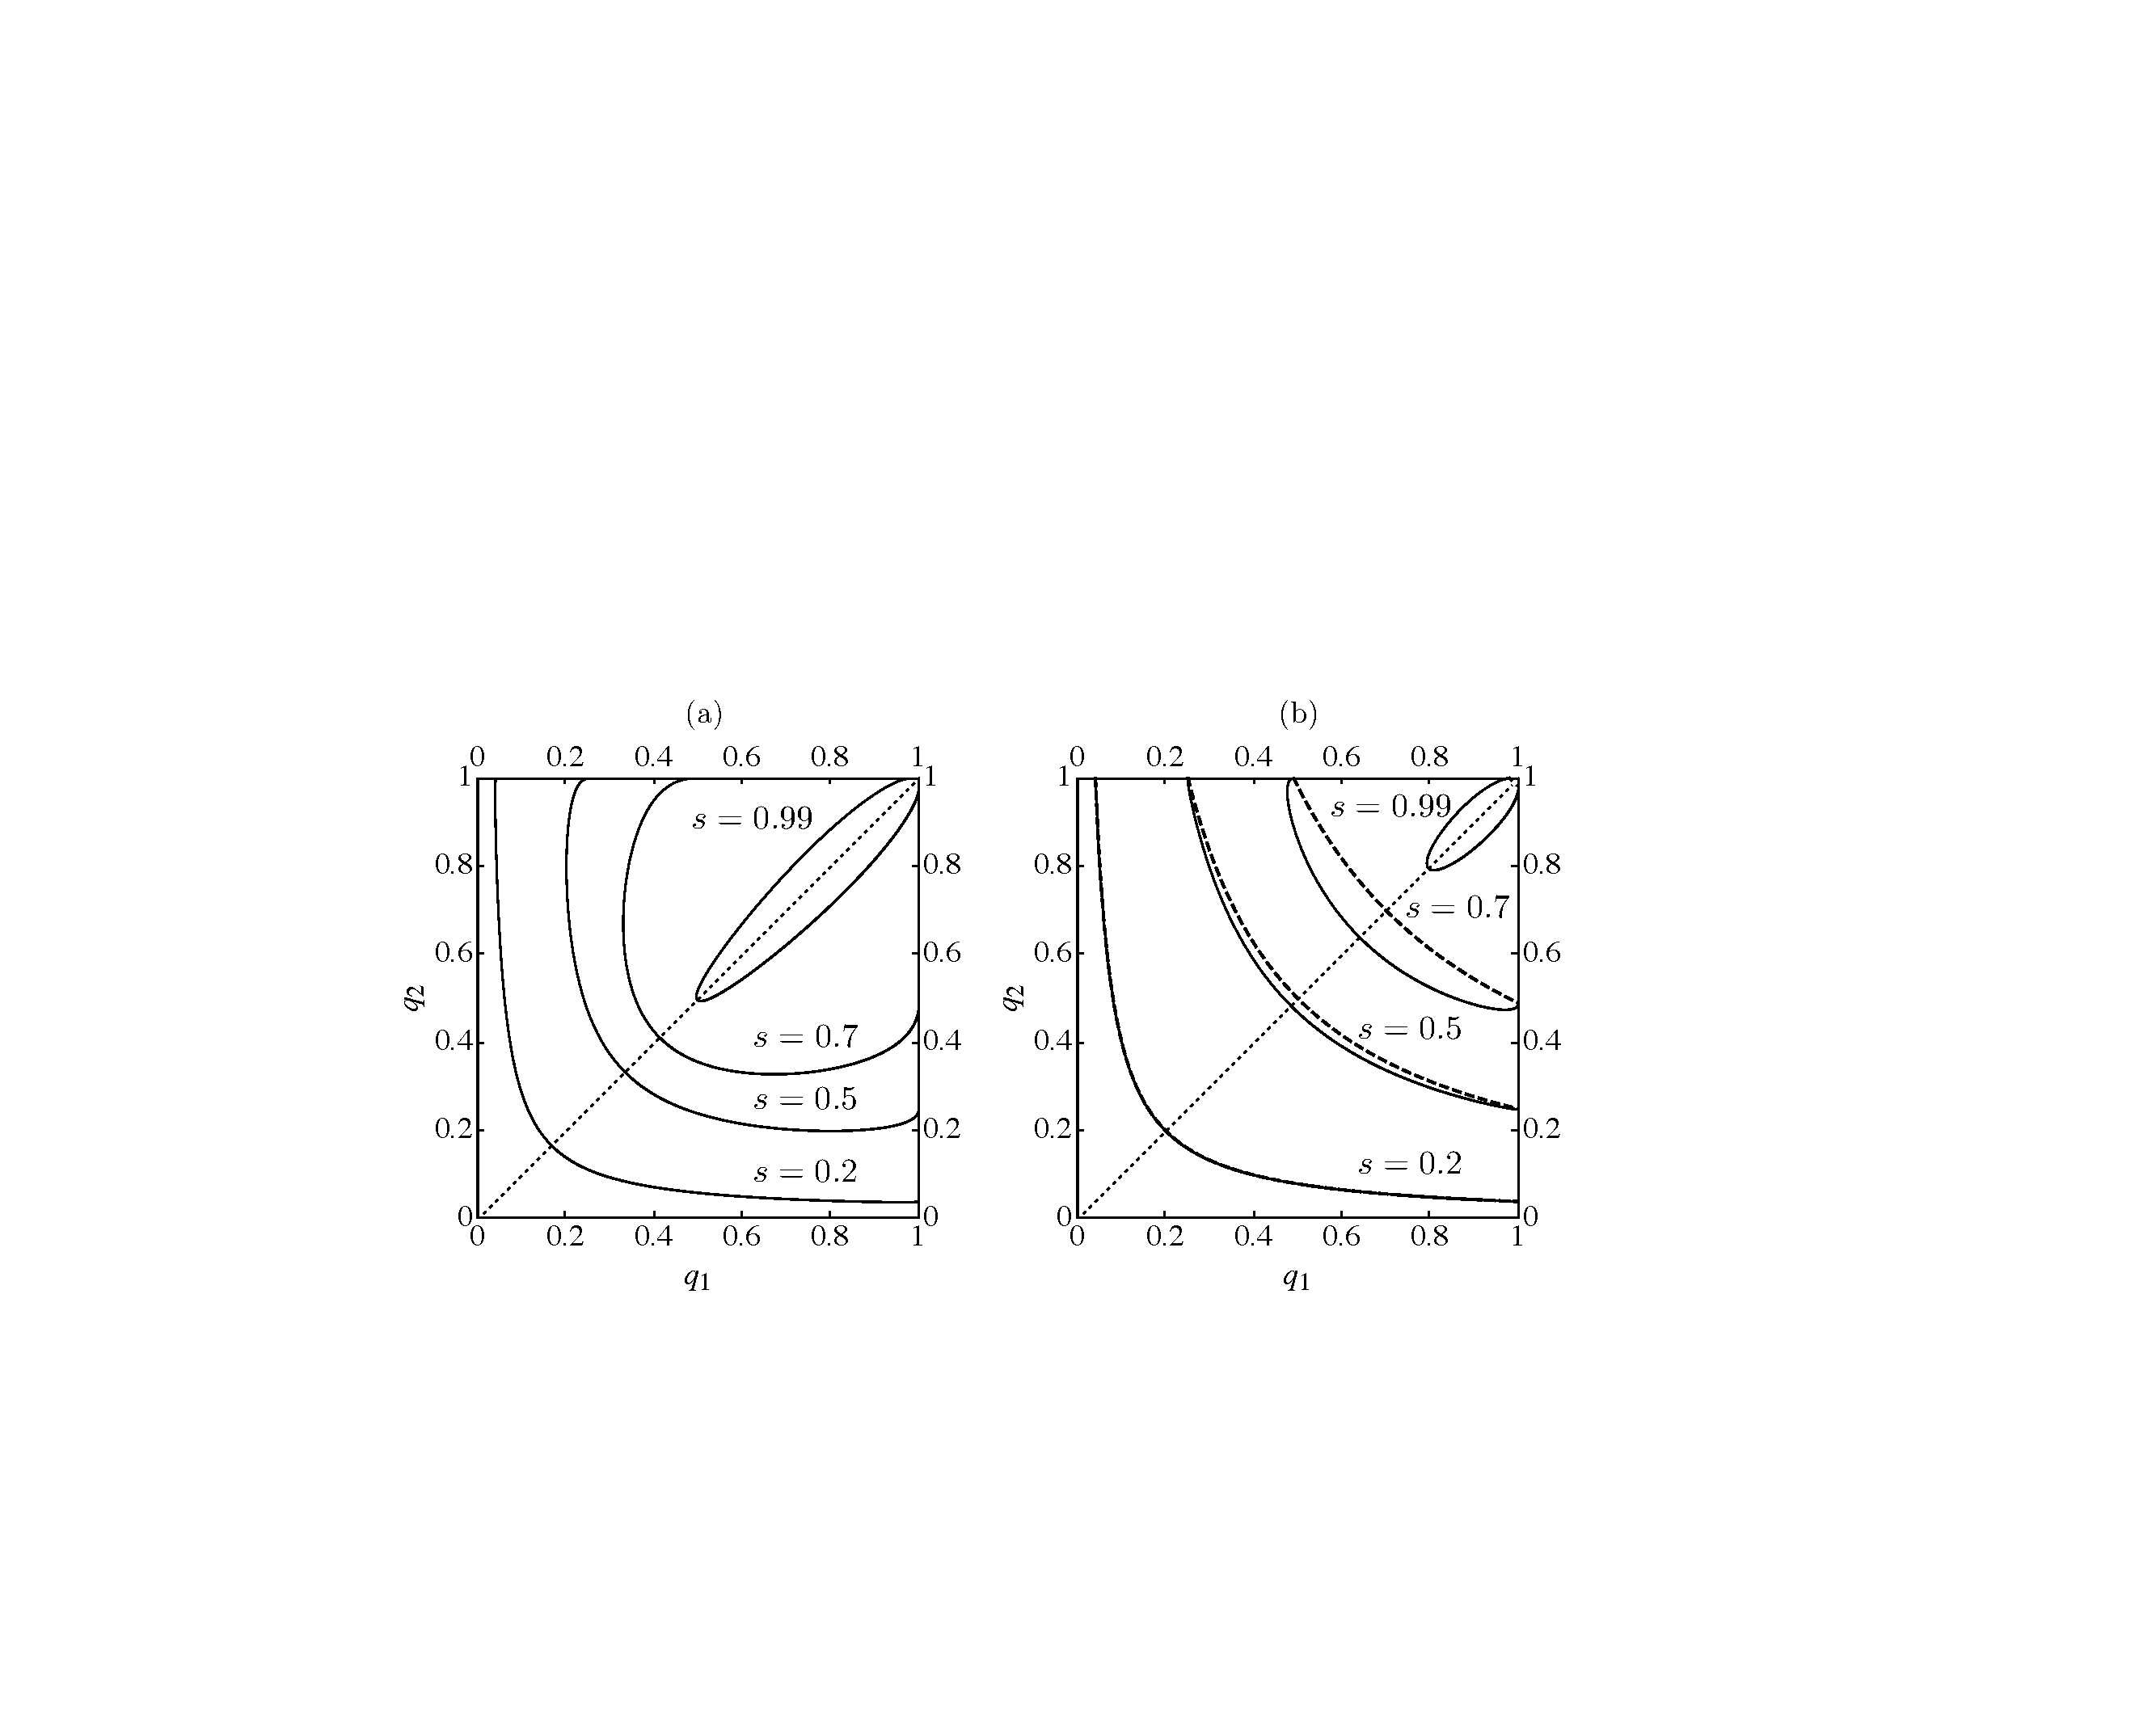
\includegraphics[width=26.8em]{Fig_2NC.pdf}\\
\end{array}%
$%
\caption{Unitarity curves, $q_{2}$ vs. $q_{1}$, from Eq.~(\ref{unit cond}) for different values of~$s$ and for (a) $m=1$, $n=2$ and (b) $m=1$, $n=5$. The curves are symmetric under mirror reflection along the dotted line $q_1=q_2$, i.e., under the transformation~$q_1\leftrightarrow q_2$. The dashed lines in~(b) are the hyperbolae~$q_1 q_2=s^{2m}$.}
\label{fig:2}
\end{figure}

For $n > 2$ the curves closely approximate $q_1 q_2=s^{2m}$ (dashed lines) for small and moderate values of $s$, while for $s$ close to $1$ the hyperbolas remain closer to the vertex~$(1,1)$, but retain the same end points. In the limit~$n\to\infty$ all these curves become hyperbolic.
%%%%%%%%%%%%%%%%%%%%%%%%%%%%%%%%%%%%%%%%%%%%%%%%
%%%%%%%%%%%%%%%%%%%%%%%%%%%%%%%%%%%%%%%%%%%%%%%%
\subsection{Optimization}
We now return to finding the minimum, $Q_{\rm min}$, of the average failure probability $Q$. Despite its apparent simplicity, this involves solving a high-order equation without a simple form. Instead, we will derive a parametric equation for $Q_{\rm min}(\eta_1)$. Along with the complete description of the unitary curve~(\ref{unit cond}), this provides a complete solution of the problem in parametric form.

With no loss of generality we may assume $\eta_1\le\eta_2$ or, equivalently,  $0\le\eta_1\le 1/2$. Then the slope of the straight line~(\ref{obj fun}), $-\eta_{1}/ \eta_{2}$, satisfies $-1\leq -\eta_{1}/\eta_{2} \leq0$. Hence, it can only become tangent to the lower half of the unitarity curve~(\ref{unit cond}) (see Fig.~\ref{fig:2}). 
Increasing $q_{1}$, the slope of this lower half increases monotonically from $-1$ at $q_1=q_2$, to $0$ before we reach the line~$q_1=1$ (assuming $n$ is finite). This follows from the properties (a)--(f) above and can be checked using  Eq.~(\ref{par sqrt}). The values of $t$ at which the slope is $-1$ and $0$ are, respectively,
%
\begin{equation}
t_{-1}=\frac{1-s^{n-m}}{1-s^n},\quad
t_0=\frac{1-s^{2(n-m)}}{1-s^{2n}}.
\label{t's}
\end{equation}
%
For any point $(q_1(t),q_2(t))$ with $t\in[t_{-1},t_0]$ there is a line $Q=\eta_1 q_1+\eta_2 q_2$ that is tangent to it, starting with $\eta_1=\eta_2=1/2$ for $t=t_{-1}$ up to $\eta_1=0$, $\eta_2=1$ for $t=t_0$. 
It is convenient to represent this class of lines with slope $-{\eta_1 \over \eta_2}$ that represent the failure rate $Q$ by using its normal vector $\vec n=(\eta_1,\eta_2)$. From this set of admissable solutions, the minimum Q is the is the line in this class that intersects the unitarity curve once, and hence is tangent to it.  This tangency can also be represented by a normal vector, 
\begin{equation}
\vec t = ({-dq_2\over dt},{dq_1 \over dt})
\end{equation}
For optimality we know the two tangent vectors must be parallel: $\hat n = \hat t$.

We can express the line tangent to the unitary curve as $\eta_1 q'_1+\eta_2 q'_2=0$, where the primed variables are derivates with respect to $t$.  Using the constraint $1=\eta_1+\eta_2$ we have 
\begin{equation}
\eta_1={q'_2\over q'_2-q'_1},\quad \eta_2={q'_1\over q'_1-q'_2}.
\end{equation}
We could solve these equations for $t(\eta_1)$ and substitute into $q_1$ for the explicit expression if it were not a high order expression.  Numerically this is easily achieved.

This observation enables us to derive the desired parametric expression for the optimality curve~$Q_{\rm min}(\eta_1)$ as follows. For a given $t$ in the range above, a necessary condition for tangency is \mbox{$\eta_1 q'_1+\eta_2 q'_2=0$}, where $q'_i=d q_i/d t$. In this equation we can solve for $\eta_1$ (or $\eta_2$) using that~$\eta_1+\eta_2=1$. By substituting $q_1$ and~$q_2$ in Eq.~(\ref{obj fun}) with~(\ref{par sqrt}) we enforce contact with the unitarity curve and obtain the expression of $Q_{\rm min}$. The final result can be cast as:

%
\begin{equation}
\eta_1=\frac{q'_2}{q'_2-q'_1},\;\; Q_{\rm min}=\frac{q'_2 q_1-q'_1 q_2}{q'_2-q'_1},\;\; t_{-1}\le t\le t_0,
\label{main}
\end{equation}
%
where $t_{-1}$, $t_0$ and $q_i$ are given in Eqs.~(\ref{t's}) and~(\ref{par sqrt}). The expressions for the derivatives $q'_i$ are
%
\begin{equation}
q'_i=\frac{\sqrt{q_i(1-q_i)}}{s^{n-m}}\left\{\frac{1+s^n}{\sqrt{1-x^2}}-(-1)^i\frac{1-s^n}{\sqrt{1-y^2}}\right\}.
\label{qi'}
\end{equation}
%
\subsection{Relation of perfect cloning with discrimination}

Fig.~\ref{fig:3} shows plots of the curves $Q_{\rm min}(\eta_1)$ for $m=1$ input copies and  (a) $n=2$ or (b) $n=5$ clones, as in the previous figure. We see that $Q_{\rm min}$ is an increasing function of $\eta_1$ in the given range $[0,1/2]$. The values of~$Q_{\rm min}$ at the end points of this range follow by substituting $t_{0}$ and $t_{-1}$, Eq.~(\ref{t's}), into Eq.~(\ref{par sqrt}). They are given by
%
\begin{equation}
Q_{0}=q_2(t_0)=\frac{s^{2m}-s^{2n}}{1-s^{2n}},\quad
Q_{-1}=\frac{s^m-s^n}{1-s^n},
\label{Q's}
\end{equation}
%
where $Q_{\rm min}=Q_{-1}$ holds for equal priors and $Q_{\rm min}=Q_0$ for $\eta_1\to 0$ (i.e., $\eta_2\to 1$).
\begin{figure}[ht]
\centering
$%
\begin{array}{c}
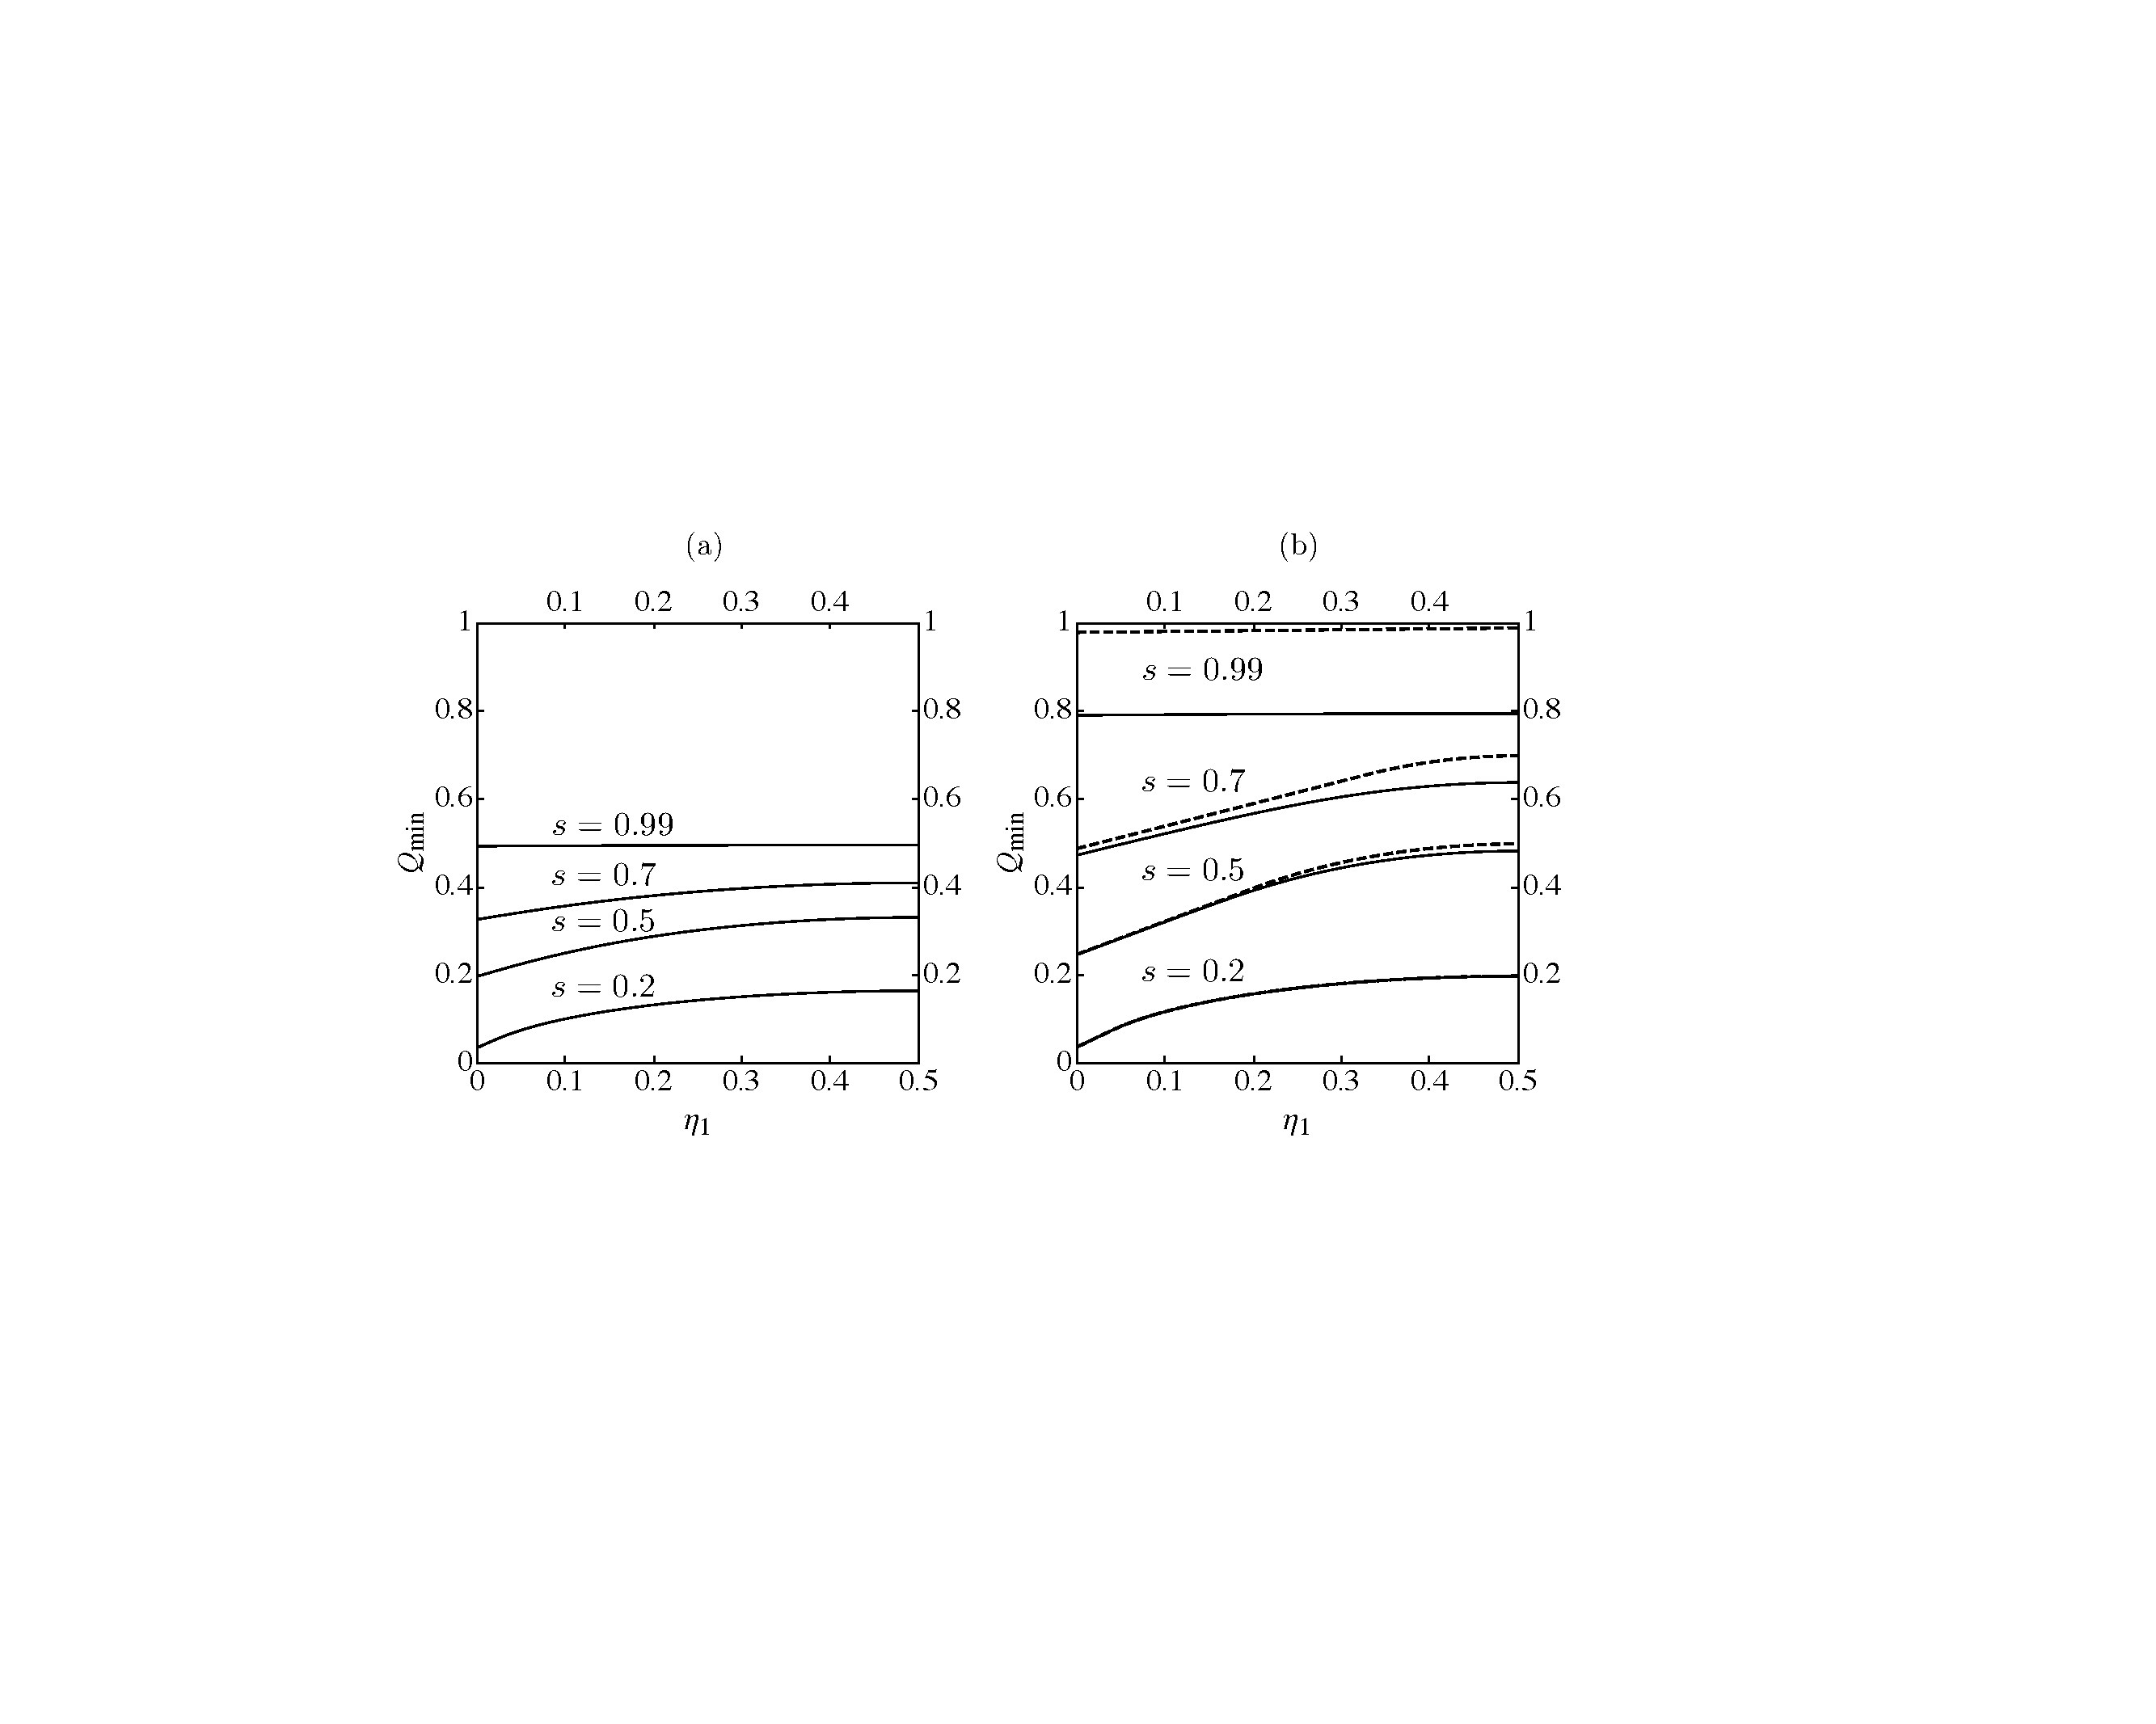
\includegraphics[width=26.7em]{Fig_3NC.pdf}\\
\end{array}%
$%
\caption{Minimum cloning failure probability $Q_{\rm min}$ vs. $\eta_1$ (solid lines) and~UD failure probability $Q_{\rm UD}$ vs. $\eta_1$ (dashed lines) for the same values of $m$, $n$ and $s$ used in the previous figure.}
\label{fig:3}
\end{figure}
The dashed lines in Fig.~\ref{fig:3}~(b) depict the well known optimal UD solution~\cite{Bergou}:
%
{
\begin{equation}
Q_{\rm UD}=\left\{
\begin{array}{ll}
2\sqrt{\eta_1\eta_2}\, s^m,&\displaystyle \frac{s^{2m}}{1+s^{2m}}\le\eta_1\le \frac{1}{2};\\[.5em]
\eta_1+s^{2m} \eta_2, \quad &\displaystyle 0\le \eta_1\le \frac{s^{2m}}{1+s^{2m}}.
\end{array}
\right.
\label{UD}
\end{equation}
}
%

It is apparent from these plots that the optimal cloning protocol performs strictly better than cloning by discrimination, as was geometricaly proved in Figs. \ref{fig:1} and \ref{fig:2}. However, the difference in performance decreases with increasing number of clones. In Fig.~\ref{fig:3}~(b), for only $n=5$, a difference is hardly noticeable for $s\le 0.5$. For $s > 0.5$ the convergence is slower but in the limit $n\to\infty$ there is perfect agreement for any $s<1$.

The convergence of the optimal cloning failure probability, $Q_{\rm min}$, to that of cloning by discrimination, $Q_{\rm UD}$ in Eq.~(\ref{UD})
follows from our geometrical approach. Recall that in the limit $n\to\infty$ (or equivalently $\alpha\to0$)  the right hand side of Eq.~(\ref{unit cond}) describes hyperbolas that we can write as $q_2=s^{2m}/q_1$ (dashed lines in Figs.~\ref{fig:1} and~\ref{fig:2}). Their  slopes are in the range $[-1,-s^{2n}]$.  A unique point of tangency with the line~(\ref{obj fun}) can only exists if the slope of this line, $-\eta_1/\eta_2$, is within this same range. This gives the $\eta_1$ interval in the first line of~(\ref{UD}), and one can easily obtain the corresponding expression for~$Q_{\rm UD}$.
%
If the slope of the line~(\ref{obj fun}) is outside the range, tangency is not possible, and the optimal line merely touches the end points of the hyperbolas, so the expression of~$Q_{\rm UD}$ becomes the second line of Eq.~(\ref{UD}). In geometrical terms, the straight line~(\ref{obj fun}) pivots on the end points as we vary~$\eta_1$. Furthermore, note that for the second line in~(\ref{UD}) we have $p_1=1-q_1=0$, which leads to a $2$-outcome projective measurement, as only one success flag state ($|\alpha_2\rangle$) is needed in Eqs.~(\ref{Ui}). 

Interestingly, in this limit a phenomenon analogous to a second order phase transition takes place. Our geometrical approach shows that the average failure probability $Q_{\rm min}(\eta_1)$ is an infinitely differentiable function of~$\eta_1$ for finite $n$. However, as $n$ goes to infinity (or $\alpha\to0$) the limiting function $Q_{\rm UD}(\eta_1)$ has a discontinuous second derivative. Moreover, the symmetry $q_1\leftrightarrow q_2$ breaks  in the ``phase" corresponding to the second line in Eq.~(\ref{UD}). A~similar phenomenon arises in UD of more than two pure states~\cite{Bergou1}.

It has been argued above that cloning by discrimination is strictly suboptimal (unless $n\to \infty$).
One could likewise wonder if discrimination by cloning can be optimal. On heuristic grounds, one should not expect this to be so, as cloning involves a measurement and some information can be drawn from the observed outcome. However, the equal-prior and the $\eta_1\to 0$ cases provide remarkable exceptions. For both we may write the total failure rate as $Q_{\rm C} + (1-Q_{\rm C})Q_{\rm UD}$, where C stands for cloning. For $\eta_1 = \eta_2= 1/2$, Eq.~(\ref{Q's}) implies $Q_{\rm C}=Q_{-1}$, in which case the produced $n$-clone states are equally likely. The UD of these states fails with probability $s^{n}$, as follows from Eq.~(\ref{UD}) applied to $n$ copies. The total failure rate is then $s^m$, which is the optimal UD failure rate of the original input states, Eq.~(\ref{UD}). If $\eta_1\to 0$ then only $|\psi^n_2\rangle$ is produced with non-vanishing probability and  $Q_{\rm C}=Q_{0}$. Failure in the second step (UD) is given by the bottom line in Eq.~(\ref{UD}) applied to $n$ copies. The total failure rate is $s^{2m}$, also achieving optimality. 

Using our main result in Eqs.~(\ref{main}), and~(\ref{par sqrt}) one can check that these are the only cases where discrimination by cloning is optimal. These are also the only cases where no information gain can be drawn from the cloning measurement.  This hints at how special these cases are and justifies the need of the derived solution for arbitrary priors to have a full account of two-state cloning. 
%%%%%%%%%%%%%%%%%%%%%%%%%%%%%%%%%%%%%%%%%%%%%%%%
%%%%%%%%%%%%%%%%%%%%%%%%%%%%%%%%%%%%%%%%%%%%%%%%
%%%%%%%%%%%%%%%%%%%%%%%%%%%%%%%%%%%%%%%%%%%%%%%%
%%%%%%%%%%%%%%%%%%%%%%%%%%%%%%%%%%%%%%%%%%%%%%%%
%%%%%%%%%%%%%%%%%%%%%%%%%%%%%%%%%%%%%%%%%%%%%%%%
%%%%%%%%%%%%%%%%%%%%%%%%%%%%%%%%%%%%%%%%%%%%%%%%
%%%%%%%%%%%%%%%%%%%%%%%%%%%%%%%%%%%%%%%%%%%%%%%%
%%%%%%%%%%%%%%%%%%%%%%%%%%%%%%%%%%%%%%%%%%%%%%%%
\section{Interpolative Cloning}

In this section we seek to interpolate between probabilistic exact
cloning and approximate cloning machines using our results from state
separation. Exact cloning machines produce perfect clones while allowing
for some inconclusive outcomes. Approximate cloning machines produce
copies on demand which resemble the input states by maximizing the
fidelity. One can imagine a scheme where fidelity can be higher then
maximum fidelity in the approximate cloning machine while it allows
for a fixed rate of inconclusive outcomes, FRIO. This scheme should
reproduce exact cloning and approximate cloning machines by setting
FRIO to $Q_{o}$ and zero respectively. Chefles and Barnett \cite{Chefles1999}
solved the problem for the case when the input states are prepared
with equal a priori probabilities. We extend the solution to the more
general case when the states are prepared with different priors. Such
a solution is possible due to our recent work on making $N$ perfect
clones from $M$ copies of one of two known pure states with minimum
failure probability in the general case where the known states have
arbitrary priori probabilities.

%%%%%%%%%%%%%%%%%%%%%%%%%%%%%%%%%%%%%%%%%%%%%%%%
%%%%%%%%%%%%%%%%%%%%%%%%%%%%%%%%%%%%%%%%%%%%%%%%
\subsection{Equal priors}

The solution to the interpolation of cloning for equal a priori probabilities
has been derived by Chefles et al \cite{Chefles1999}. The authors
develop a scheme which, depending on the fidelity of the clones, can
interpolate between exact cloning with inconclusive results in one
extreme and optimal approximate cloning on the other extreme. In our
work this scheme has been generalized for the case when the input
states are prepared with different a priori probabilities. First we
show the derivation of the equal priors as it will help to better
understand the general case. 

For $\eta_{1}=\eta_{2}=1/2,$ the output states are symmetric, $\phi_{1}=\phi_{2}=\phi,$
and the optimal global fidelity, $F_{MN}$, in Eq.(\ref{eq:fid})
reduces to: 

\begin{eqnarray}
F_{MN} & = & \frac{1}{2}\left[1+\sqrt{1-\sin^{2}\left(2\theta-2\phi\right)}\right],\nonumber \\
 & = & \frac{1}{2}\left[1+\cos^{2}\left(2\theta-2\phi\right)\right].\\
\nonumber 
\end{eqnarray}
 

Duan and Guo \cite{Duan1998} showed that the maximum success probability
of obtaining $N$ exact clones from $M$ given copies of non-orthogonal
quantum states $\{|\psi_{1}\rangle,|\psi_{2}\rangle\}$, which are
prepared with equal a priori probabilities, is:

\begin{equation}
P_{MN}=\frac{1-s^{M}}{1-s^{N}},
\end{equation}
where $s$ is the overlap of the input states $s=\langle\psi_{1}|\psi_{2}\rangle.$
The success rate for 1 to 2 cloning, $M=1,N=2,$ reduces to:

\begin{equation}
P_{12}=\frac{1}{1+s}.
\end{equation}
The interpolation takes us from optimal exact cloning to maximum fidelity.
Given a set $K$ of two non-orthogonal quantum states, $\{|\psi_{1}\rangle,|\psi_{2}\rangle\}$
the goal is to make $N$ clones $\{|\phi_{1}\rangle,|\phi_{2}\rangle\}$,
which are similar to the input states but not perfect. The Neumark
setup is:

\begin{eqnarray}
U|\psi_{1}\rangle^{\otimes M}|i\rangle & = & \sqrt{p}|\phi_{1}\rangle^{\oplus N}|1\rangle+\sqrt{q}|f\rangle|0\rangle\label{eq:NeumarkClone1}\\
U|\psi_{2}\rangle^{\oplus M}|i\rangle & = & \sqrt{p}|\phi_{2}\rangle^{\oplus N}|1\rangle+\sqrt{q}|f\rangle|0\rangle\label{eq:NeumarkClone2}
\end{eqnarray}


The input states are prepared with equal a priori probabilities. A
click in the $|1\rangle$ direction means that we succeed in making
the clones and the probability of success is $p.$ A click in the
$|0\rangle$ direction means that we failed to create a clone with
a probability $q.$ The inner product or (\ref{eq:NeumarkClone1})
and (\ref{eq:NeumarkClone2}) gives the constraint: 

\begin{equation}
s^{M}=ps'^{N}+q
\end{equation}


Using the unitarity condition $p+q=1,$ the average rate of successfully
making a clone is:

\begin{equation}
p=\frac{1-s^{M}}{1-s'^{N}}
\end{equation}


$s'$ is the overlap of the clones $s'=\langle\phi_{1}|\phi_{2}\rangle$.
If the final states are orthogonal, $s'=0$ then the state separation
reaches the IDP limit and $P_{S}=P_{IDP}=1-|\langle\psi_{1}|\psi_{2}\rangle|^{M}.$ 

First we express the overlap of the output states in terms on the
success rates and the overlap of input states, $\cos2\theta=|\langle\psi_{1}|\psi_{2}\rangle|^{N}$

\begin{eqnarray}
|\langle\phi_{1}|\phi_{2}\rangle|^{N} & = & 1-\frac{1-|\langle\psi_{1}|\psi_{2}\rangle|^{M}}{P_{S}}\\
\cos^{N}(\phi_{1}+\phi_{2}) & = & 1-\frac{P_{IDP}}{P_{S}}\label{eq:seperation}
\end{eqnarray}
The exact clones live in an N dimensional space $|\psi_{1,2}^{N}\rangle=\cos\theta|1\rangle\pm\sin\theta|0\rangle.$
The approximate clones can be expressed as $|\phi_{1,2}\rangle=\cos\phi_{1}|1\rangle\pm\sin\phi_{1}|0\rangle$.

The fidelity rate for equal priors is:

\begin{equation}
F_{MN}=\frac{1}{2}\left[1+\cos(2\theta-\left(\phi_{1}+\phi_{2}\right)\right],
\end{equation}
 and we want to use the relationship in (\ref{eq:seperation}). Let
us expand the cosine term 

$\cos\left(2\theta-\left(\phi_{1}+\phi_{2}\right)\right)=\cos2\theta\cos\left(\phi_{1}+\phi_{2}\right)+\sin2\theta\sin\left(\phi_{1}+\phi_{2}\right).$

The fidelity becomes:

\begin{eqnarray*}
\\
F_{MN} & = & \frac{1}{2}\left[1+|\langle\psi_{1}^{N}|\psi_{2}^{N}\rangle|\left(1-\frac{P_{IDP}}{P_{S}}\right)+\frac{1}{P_{S}}(\left(1-|\langle\psi_{1}^{N}|\psi_{2}^{N}\rangle|^{2}\right)\left(P_{S}^{2}-\left(P_{S}-P_{IDP}\right)^{2}\right)^{1/2}\right]
\end{eqnarray*}
 As $N\rightarrow\infty,\thinspace|\langle\psi_{1}|\psi_{2}\rangle|^{N}\rightarrow0$
and $F_{MN}$ reduces to

\[
F_{MN}=\frac{1}{2}[1+\frac{1}{P_{S}}\sqrt{P_{S}^{2}-(P_{S}-P_{IDP})^{2}}].
\]


We can also express the fidelity in terms of fixed failure rate $Q=1-P_{S}$
which serves as the parameter by which we are interpolating and the
optimal failure rate $Q_{o}=\left|\langle\psi_{1}|\psi_{2}\rangle\right|$ 

\begin{eqnarray*}
F_{MN} & = & \frac{1}{2}\left[1+|\langle\psi_{1}^{N}|\psi_{2}^{N}\rangle|(1-\frac{1-Q_{o}}{1-Q})+\frac{1}{1-Q}(\left(1-|\langle\psi_{1}^{N}|\psi_{2}^{N}\rangle|^{2}\right)\left(\left(1-Q\right)^{2}-(Q-Q_{o})^{2}\right)^{1/2}\right],\\
 & = & \frac{1}{2\left(1-Q\right)}\left[(1-Q)+Q_{o}^{N}(Q_{o}-Q)+\sqrt{(1-Q_{o}^{2N})\left[(1-Q)^{2}-(Q-Q_{o})^{2}\right]}\right].
\end{eqnarray*}
In the limit $N\rightarrow\infty,\thinspace|\langle\psi_{1}|\psi_{2}\rangle|^{N}\rightarrow0$ 

\begin{eqnarray*}
F_{MN} & = & \frac{1}{2}\left[1+\frac{1}{1-Q}\sqrt{(1-Q)^{2}-(Q-Q_{o})^{2}}\right],\\
(1-Q)F_{MN} & = & \frac{1}{2}\left[(1-Q)+\sqrt{(1-Q)^{2}-(Q-Q_{o})^{2}}\right].
\end{eqnarray*}
$(1-Q)F_{MN}=P_{succes}$, the probability of successfully identifying
a state. 

\begin{eqnarray*}
P_{success} & = & \frac{1}{2}[(1-Q)+\sqrt{(1-Q)^{2}-(Q-Q_{o})^{2}}]
\end{eqnarray*}
(This is a different success rate then the $P_{S}$ defined above,
the $P_{S}$ was defined as the rate of successfully carrying out
a state separation. )

This formula describes the relationship between the discrimination
of states with a fixed rate of inconclusive outcome. When $Q=0$ it
reaches the Helstrom bound of minimum error and when $Q=Q_{o}$ it
reaches the IDP limit in UD. 

%%%%%%%%%%%%%%%%%%%%%%%%%%%%%%%%%%%%%%%%%%%%%%%%
%%%%%%%%%%%%%%%%%%%%%%%%%%%%%%%%%%%%%%%%%%%%%%%%
\subsection{General case}

We would like to generalize the above results for the case when the
incoming states are prepared with different prior probabilities. 
\begin{itemize}
\item Step 1: State Separation
\end{itemize}
Optimally separate the incoming states $\left\{ \ket{\psi_{1}^{M}},\ket{\psi_{2}^{M}}\right\} $
with a fixed rate of inconclusive results $q_{i}$, then prepare states
$\left\{ \ket{\psi_{1}^{N}},\ket{\psi_{2}^{N}}\right\} $ with the
corresponding success probabilities. 

\begin{eqnarray}
U|\psi_{1}^{M}\rangle|0\rangle & = & \sqrt{p_{1}}|\phi_{1}\rangle|1\rangle+\sqrt{q_{1}}|\Phi\rangle|2\rangle,\nonumber \\
U|\psi_{2}^{M}\rangle|0\rangle & = & \sqrt{p_{2}}|\phi_{2}\rangle|1\rangle+\sqrt{q_{2}}|\Phi\rangle|2\rangle,
\end{eqnarray}


The incoming states are separated with a success probability $p_{i}$
and failed to separate the states with a failure probability $q_{i}$.
The inner product of the two equations gives the unitarity constraint

\begin{equation}
s=\sqrt{p_{1}p_{2}}s'+\sqrt{q_{1}q_{2}}\label{eq:setaration constraint}
\end{equation}

\begin{itemize}
\item Step 2: Optimize Fidelity
\end{itemize}
The fidelity for state $\ket{\psi_{1}}$ is: $F_{1}=\left|\braket{\psi_{1}^{N}}{\phi_{1}}\right|^{2}$.
Similarly the fidelity for state $\ket{\psi_{2}}$is $\left|\braket{\psi_{2}^{N}}{\phi_{2}}\right|^{2}$.
The overall fidelity is

\[
F=\frac{\eta_{1}p_{1}F_{1}+\eta_{2}p_{2}F_{2}}{\eta_{1}p_{1}+\eta_{2}p_{2}}=\frac{\eta_{1}p_{1}F_{1}+\eta_{2}p_{2}F_{2}}{1-Q}=\tilde{\eta}_{1}F_{1}+\tilde{\eta}_{2}F_{2},
\]
where the normalized a priori probabilities are $\tilde{\eta}_{i}=\frac{\eta_{i}p_{i}}{1-Q}$.
The average fidelity is the same as calculated in (\ref{eq:fid})
with the new normalized probabilities: 

\begin{eqnarray}
F_{MN} & = & \frac{1}{2}\left[1+\sqrt{1-4\tilde{\eta}_{1}\tilde{\eta}_{2}\sin^{2}\left(2\theta-\left(\phi_{1}+\phi_{2}\right)\right)}\right],\nonumber \\
 & = & \frac{1}{2(1-Q)}\left[(1-Q)+\sqrt{\left(1-Q\right)^{2}-4\eta_{1}\eta_{2}p_{1}p_{2}\sin^{2}\left(2\theta-\left(\phi_{1}+\phi_{2}\right)\right)}\right],
\end{eqnarray}


It can be seen that in the limit $N\rightarrow\infty$, expanding
the $\sin$ term as we did in the previous section, the FRIO \cite{Bagan2012}
results are recovered. It again shows a close relationship between
fidelity and state discrimination. 

Solving the problem of hybrid cloning however requires one last optimization,
that of the second term under the square root

\begin{equation*}
\Lambda  =  \sqrt{p_{1}p_{2}}\sin\left(2\theta-\left(\phi_{1}+\phi_{2}\right)\right),\\
 \end{equation*}
We can write its optimal value of $\Lambda$ in terms of the constrained variables of state separation $u$ and $v$, which will be discussed in the following chapter, as
\begin{equation}
\Lambda_{\rm min}= \sqrt{1-s^{2n}}\left(s-u\right)-s^{n}\sqrt{1-s^{2}-2v+2su}.
\end{equation}
Here $u\equiv\sqrt{q_{1}q_{2}},\hspace{0.5cm}v\equiv\frac{1}{2}\left(q_{1}+q_{2}\right)$
and we used the constraint from the unitarity in (\ref{eq:separation constraint})
to replace $\sqrt{p_{1}p_{2}}s'=s-\sqrt{q_{1}q_{2}}$. In terms of the trigonometric variables this is
\begin{equation}
\Lambda_{\rm min} = \sqrt{1-s^{2n}}(s-\frac{Q \cos(\theta)}{\sqrt{1-\delta^2}})-s^n\sqrt{\frac{2Q-(-1+s^2)(-1+\Delta^2) -2 Q s \sqrt{1-\Delta^2} \cos (\theta)+2Q \Delta \sin(\theta)}{-1 +\Delta^2}}
\end{equation}
To find its minimum we use two equations; for the first we differentiate $\frac{\partial \Lambda_{\rm min}}{\partial u} = \frac{\partial v}{\partial u}$ and for the second $v = \Lambda_{\rm min}$ to get two master equations that we can solve for any two parameters in terms of $\theta$. 
\begin{eqnarray*}
0=\frac{s^{-n} \left(\cot (\theta ) s^{2 n} (\Delta +Q \sin (\theta ))+\sqrt{1-\Delta ^2} \left(s-\varphi  \sqrt{1-s^{2 n}}\right)-Q \cos (\theta )\right)}{\sqrt{1-\Delta ^2}}\\
0=\frac{1}{2} s^{-2 n} \left(\frac{Q^2 \cos ^2(\theta ) \left(s^{2 n}-1\right)}{\Delta ^2-1}-\frac{2 Q \cos (\theta ) \left(s-\varphi  \sqrt{1-s^{2 n}}\right)}{\sqrt{1-\Delta ^2}}-2 s \varphi  \sqrt{1-s^{2 n}}-s^{2 n}+s^2+\varphi ^2\right)\\
+\frac{\Delta  Q \sin (\theta )+Q}{1-\Delta ^2}
\end{eqnarray*}

This completes the solution to the approximate probabilistic cloning problem.  To better understand these equations and their implications we will turn our attention to the problem of state separation.  For optimal cloning we saw an objective function that was a fidelity and the constraints a unitarity equation along with the fixed average failure rate.  We maximized the fidelity for a given failure rate, but we can readily solve the equations for the failure rate and final overlap as functions of the remaining variables.  We will see this feature explored in detail.

%%%%%%%%%%%%%%%%%%%%%%%%%%%%%%%%%%%%%%%%%%%%%%%%
%%%%%%%%%%%%%%%%%%%%%%%%%%%%%%%%%%%%%%%%%%%%%%%%
%%%%%%%%%%%%%%%%%%%%%%%%%%%%%%%%%%%%%%%%%%%%%%%%
%%%%%%%%%%%%%%%%%%%%%%%%%%%%%%%%%%%%%%%%%%%%%%%%
\chapter{State Separation}

While reading through the section on perfect cloning one may have thought it is an obvious generalization to choose a variable parameter $s'$ for output overlap instead of a fixed $\bk{\psi_1}{\psi_2}^N$ because it is simply the more general problem.  In fact, since any quantum transformation must obey unitary evolution, the unitarity equation places strict bounds on a system coupled with an ancilla in hopes of increasing its overlap.  This includes all possible transformations no matter the protocol or designation.  Therefore we should expect that the equations for state separation coincide with the studied measurement strategies in particular bounds.  When addressing this question we wish to be as rigorous as possible and not let uwary assumptions limit our solutions, particularly those we took for granted in discrimination and cloning.

We can again start by imagining that a probabilistic quantum transformation is carried out by a machine with an input port, an output port and two flags that herald the success or failure of the transformation.  The input $|\psi_i\rangle$, $i=1,2$ is fed through the input port for processing. In case of success, states~$|\psi'_i\rangle$, with the desired degree of separation, are delivered through the output port with conditioned probability~$p_i$. Otherwise, the output is in a failure state. Conditioned on the input state being $|\psi_i\rangle$, the failure probability is~$q_i=1-p_i$. 

We address optimality from a Bayesian viewpoint that assumes the states to be transformed are given with some {\it a priori}  probabilities $\eta_1$ and $\eta_2$, $\eta_1+\eta_2=1$. Then a natural cost function for our probabilistic machines is given by the average failure probability 
%
\begin{equation}
Q=\eta_1 q_1+\eta_2 q_2.
\label{obj fun}
\end{equation}
%
If $|\psi_i\rangle$ and the corresponding transformed states $|\psi'_i\rangle$ are given, the optimal machine is one that minimizes the cost function 
%Accordingly, the optimal cloner is one that minimizes the cost function 
$Q$. In this case our aim is to find that optimal machine and the minimum average failure probability $Q_{\rm min}$ for arbitrary priors $\eta_1$ and $\eta_2$.
% This does {\em not} define a universal protocol. 
%The information about the two possible state preparations $|\psi_i\rangle$, their corresponding prior probabilities $\eta_i$, $i=1,2$, and transformed states~$|\psi'_i\rangle$ is hardwired into the machine. 

A different way of approaching optimality may consist in finding the machine (or machines) that achieves the highest degree of separation, namely, minimizes de overlap $s':=|\langle\psi'_1|\psi'_2\rangle|$ for given initial states $|\psi_i\rangle$, subject to the condition that the average probability~$Q$ does not exceed some given value, $Q_{\rm max}$. In this case we could further assume that either the initial overlap $s:=|\langle\psi_1|\psi_2\rangle|$ is given, in which case one can compute the tradeoff curve~$s'_{\rm min}(Q_{\rm max})$, or else assume that $Q_{\rm max}$ is fixed and compute the curve~$s'_{\min}(s)$. It is easy to see that $s'_{\rm min}(Q_{\rm max})$ and $Q_{\rm max}(s'_{\rm min})$ are just inverses of each otrher.

Whether we approach optimality one way or another depends merely on the problem at hand. Hence, e.g., for perfect cloning from one initial copies of either $|\psi_1\rangle$ or~$|\psi_2\rangle$ to $n$ final copies (i.e., $|\psi'_i\rangle=|\psi_i\rangle^{\otimes n}$), the former approach is most suitable since the final overlap is fixed, $s'=s^n$,  and so is the degree of separation attained by the cloner. So, in~\cite{us1} the solution was given in terms of~$Q_{\rm min}$ as a function of the prior probability $\eta_1$. However, one may need to know what is the maximum number of clones that can be produced if the failure rate cannot exceed~$Q_{\rm max}$, in which case one takes the latter approach, and compute $n_{\rm max}=\log[s'(Q_{\rm max})]/\log s$. 

The machine that carries the probabilistic transformation is usually described by two Kraus operators $A_{\rm succ}$, $A_{\rm fail}$, so that~$A^\dagger{}_{\kern-.3em\rm succ}A_{\rm succ}+A^\dagger{}_{\kern-.2em\rm fail}A_{\rm fail}=$~\cite{Chefles+Barnett}. We can think of $A_{\rm succ}$ and $A_{\rm fail}$ as measurement operators. The transformation is successfully applied if the outcome of such (generalized) measurement is ``succ",  and fails otherwise.
Neumark's theorem provides an alternative approach  that turns out to be more convenient for our analysis.  Additional details on this method can be found in \cite{Bergou}. 
In this formulation, %similar to that in~\cite{DuanGuo}, 
the Hilbert space ${\mathscr H}$ of the original states is supplemented with an ancillary space~${\mathscr H}_{\rm extra}\otimes {\mathscr H}_F$ that accommodates both the required extra-dimensions (if necessary) as well as the success/failure flags. Then, a unitary transformation~$U$ (time evolution) from ${\mathscr H}\otimes {\mathscr H}_{\rm extra}\otimes {\mathscr H}_{F}$ onto ${\mathscr H}'\otimes{\mathscr H}_F$ is defined through~\cite{DuanGuo}
%
\begin{eqnarray}
U|\psi_1\rangle|0\rangle&=& \sqrt{p_1}|\psi'_1\rangle|\alpha_1\rangle +\sqrt q_1 |\phi\rangle|\alpha_0\rangle,\label{U1}\\
U|\psi_2\rangle|0\rangle&=& \sqrt{p_2}|\psi'_2\rangle|\alpha_2\rangle +\sqrt q_2 |\phi\rangle|\alpha_0\rangle. \label{U2}
\end{eqnarray}
%
Here the ancillas are initialized in a reference state~$|0\rangle$. The states of the flag associated with successful transformation~$| {\alpha_i}\rangle$ are constrained to be orthogonal to the state~$|\alpha_0\rangle$ that signals failure. Upon performing a projective measurement  on the flag space ${\mathscr H}_F$, the final state delivered through the outport port of our probabilistic machine is either $|\psi'_i\rangle$, in case of success, or $|\phi\rangle$ in case of failure. So, the outcome of this measurement tells us if the machine has succeeded or failed in delivering the right transformed state.  On general grounds, optimality requires $|\alpha_1\rangle=|\alpha_2\rangle$. Here we choose to consider a more general setup where these two states are different
to include state discrimination, for which the success flag states must be fully distinguishable, so $\langle\alpha_1|\alpha_2\rangle=0$.
%
Likewise, we could consider a more general setup with two failure states $|\phi_1\rangle$ and $|\phi_2\rangle$ in Eqs.~(\ref{U1}) and~(\ref{U2}). This is necessarily sub-optimal since we could probabilistically determine whether we received $|{\psi_1}\rangle$ or $|{\psi_2}\rangle$ by applying unambiguous discrimination to the failure states~$| {\phi_i}\rangle$.  Sometimes we would be  certain of the input state, in which case we could  prepare $|\psi'_1\rangle$ or $|\psi'_2\rangle$ accordingly,  thereby increasing the overall success rate.
%
%

%From our analysis the optimality requirement $|\alpha_1\rangle=|\alpha_2\rangle$ will trivially follow.
Taking the inner product of Eqs.~(\ref{U1}) and ~(\ref{U2}) with themselves shows that our probabilities are normalized: $p_i+q_i=1$.
Similarly, by taking the product of Eq.~(\ref{U1}) with Eq.~(\ref{U2}), we find the unitarity constraint,
%
\begin{equation}
s=\sqrt{p_1 p_2}\, \beta+\sqrt{q_1 q_2},
\label{unit cond}
\end{equation}
%
where $\beta=s' |\langle \alpha_1|\alpha_2\rangle|$. Without any loss of generality, in deriving Eq.~(\ref{unit cond}) we have chosen
$\langle {\psi_1}|{\psi_2}\rangle$, $\langle {\psi'_1}|{\psi'_2}\rangle$ and~$\langle\alpha_1|\alpha_2\rangle$ to be real and positive.
%~\footnote{%
%
%
%We may choose $\alpha$ (and $\langle\Phi_1|\Phi_2\rangle=\phi$) to be real, since only their real parts show up in the unitarity condition, Eq.~(\ref{unit cond}), and the additional condition
%$$
%0=\sqrt{p_1p_2}s' \Im\,\alpha+\sqrt{q_1q_2}\Im\,\phi
%$$
%is satisfied by the choice $ \Im\,\alpha=\Im\,\phi=0$.%
%%
%%
%}
%. 
%Furthermore, we can choose $0\le s'\le s\le 1$.  
We note that $0\le\beta\le s$, and~$\beta=0$ for both full separation ($s'=0$) and unambiguous discrimination ($ |\langle \alpha_1|\alpha_2\rangle|=0$), whereas for optimal separation~$|\langle \alpha_1|\alpha_2\rangle|=1$. If Eq.~(\ref{unit cond}) is satisfied, it is not hard to prove that~$U$ has a unitary extension on the whole Hilbert space and the Kraus operators,~\mbox{$A_{\rm succ}$, $A_{\rm fail}$,} can be obtained by tracing out the ancillary degrees of freedom .

%%%%%%%%%%%%%%%%%%%%%%%%%%%%%%%%%%%%%%%%%%%%%%%%
%%%%%%%%%%%%%%%%%%%%%%%%%%%%%%%%%%%%%%%%%%%%%%%%

\section{Maximum separation}

In this section, we assume $\eta_1$, $\eta_2$ are fixed given quantities and we focus on the relationship among the initial overlap, the final overlap and the maximum allowed failure rate. To find the explicit form of these relationships, we will need to develop a new geometric view of both the unitarity constraint, Eq.~(\ref{unit cond}), and $Q= \eta_1 q_1+\eta_2 q_2$. %We aim at a simple geometry that would allow both a
We aim at a geometric representation simple enough to grasp visually the solution and yet powerful enough to provide this solution analytically. We show below that the unitary curve and the straight segment of the previous sections can be mapped into conic curves, in particular into families of parabolas and ellipses respectively. This is arguably the simplest extension to our geometric description of state separation. The desired transformation is defined in terms of the new variables $u$ and $v$ as
%
\begin{equation}
u=\sqrt{q_1 q_2};\quad v={q_1+q_2\over 2}.
\label{transf}
\end{equation}
%
They are just the geometric  and arithmetic means of the failure probabilities, $q_1$ and $q_2$. Under this transformation the unitary constraint becomes a parabola that can be conveniently written as
%
\begin{equation}
v={1+u^2\over2}-{(u-s)^2\over2s'^2}.
\label{unit cond conic}
\end{equation}
%
From this expression, one can immediately check that as~$s$ varies we obtain a family of parabolas whose envelope is yet another parabola, $v=(1+u^2)/2$, independently of $s'$. As $s'$ decreases from its maximum value $s'=s$, the parabolas in Eq.~(\ref{unit cond conic}) become thinner. For $s'=0$ they degenerate into the vertical segment $u=s$, $0\le v\le (1+s^2)/2$. These features are illustrated in~Fig.~\ref{fig:3}~(a).

Under the same transformation, Eq.~(\ref{transf}), the line $Q=\eta_1 q_1+\eta_2 q_2$ becomes an ellipse, which is most easily expressed parametrically in terms of the polar angle $\theta$, measured relative to the axis $v=0$ from the center of the ellipse. It is given by
%
\begin{eqnarray}
u&=&{Q\over\sqrt{1-\Delta^2}}\cos\theta,\nonumber\\
v&=&{Q\over1-\Delta^2}+{Q\Delta\over1-\Delta^2}\sin\theta,
\label{obj fun conic}
\end{eqnarray}
%
where we have defined $\Delta=\eta_2-\eta_1$.  %The semi-major and semi-minor axes can be read of from this equation to be 
It is clear from this expression that the eccentricity of the ellipse is only a function of the priors. For equal priors, $\Delta=0$, the ellipse degenerates into the horizontal segment $v=Q$, $0\le u\le Q$, whereas for $Q=0$ it collapses into the origin $(u,v)=(0,0)$. As one increases $Q$, a family of similar ellipses is obtained. As they increase in size, their center moves up along the axis $u=0$. The line $u=v$ is the envelope of this family, as one can easily check using~Eq.~(\ref{obj fun conic}). Fig.~\ref{fig:3}~(a) also illustrates these features.
%
\begin{figure}[t]
\centering
$%
\begin{array}{c}
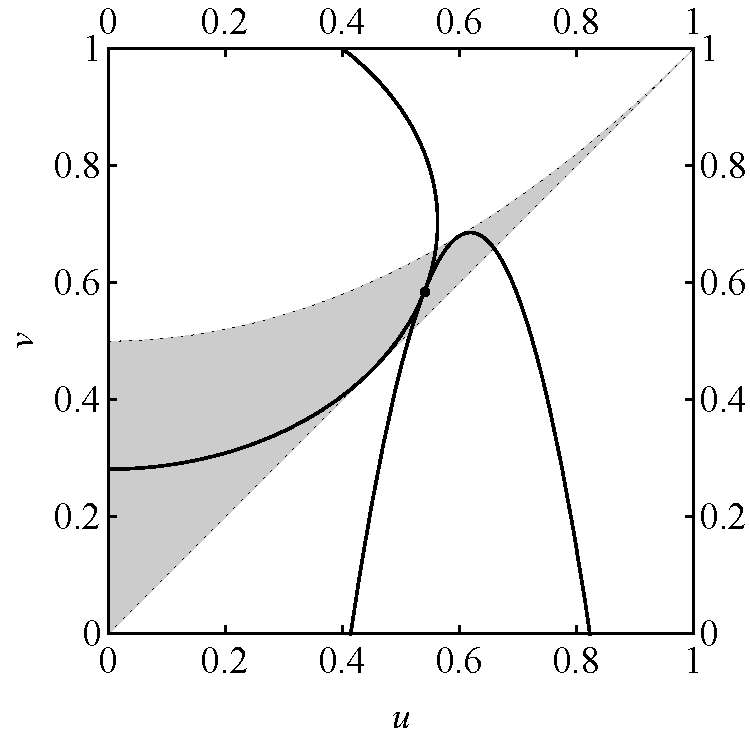
\includegraphics[width=26em]{Figures_SEPvedit.pdf}\\
\end{array}%
$%
\caption{The optimal separation point as the intersection of the parabola Eq.~(\ref{unit cond conic}) and ellipse $Q= \eta_1 q_1+\eta_2 q_2$. In this figure $\eta_1=0.2$, $s=0.6$ and $Q=Q_{\rm max}=0.45$. The optimal (minimum) value of $s'$, which gives the solid parabola, turns out to be $s'=0.17$. }
\label{fig:3}
\end{figure}
%

In terms of this conic geometry,  optimality is again given by a tangency point, this time between ellipses and parabolas. Because of the features of these families of conics, these points of tangency necessarily lie in the region between their envelopes,  which is the gray area in Fig.~\ref{fig:3}. Fig.~\ref{fig:3}~(b) illustrates optimality. Given a maximum failure rate $Q_{\rm max}$ and some initial overlap~$s$ ($Q_{\rm max}=0.35$ and $s=0.4$ in the example considered in the figure), we plot the corresponding ellipse defined by Eq.~(\ref{obj fun conic}) (dashed line). Among the various parabolas, characterized by the final overlap $s'$ (the figure shows two of them, for $s'=s$ and $s'=s/2$), the one that minimizes~$s'$ (solid line) has a unique point of tangency with the ellipse, thus giving us the solution, $s'_{\rm min}$.  To keep the notation simple we will drop the subscript ``$\rm min$'' wherever no confusion arises. 

To find the condition that gives the tangency point, we first note that the slopes of the ellipse and the parabolas are given respectively by
%
\begin{eqnarray}
{dv\over du}&=&{v'\over u'}=-{\Delta\over\sqrt{1-\Delta^2}}\cot\theta,\nonumber\\
{dv\over du}&=&u-{u-s\over s'^2},
\label{slopes}
\end{eqnarray}
%
where the prime stands for derivative with respect to the polar angle $\theta$. The right hand side of these two equations must be equal at the tangency point. Moreover, the tangency point must belong to both the ellipse and the optimal parabola. Hence
%
\begin{eqnarray}
Q{1\!+\!\Delta \sin\theta\over 1-\Delta^2}\!&=&\!{1\over2}\!+\!{Q^2\!\cos^2\theta\over2(1\!-\!\Delta^2)}
\!-\!{1\over2 s'^2}\!\!\left(\!{Q\cos\theta\over\sqrt{1\!-\!\Delta^2}}\!-\!s\!\!\right)^{\!\!2}\!\!,\nonumber
%\label{eb21.04.15-1}
\\[.5em]
%
{\Delta\cot\theta\over	\sqrt{1-\Delta^2}}&=&{1-s'^2\over s'^2}{Q\cos\theta\over\sqrt{1-\Delta^2}}-{s\over s'^2}.
\label{eb21.04.15-2}
\end{eqnarray}
%
where to obtain the first (second) equation we have simply substituted Eq.~(\ref{obj fun conic}) into Eq.~(\ref{unit cond conic}) [Eq.~(\ref{slopes})].
Ideally, we would like to solve this system of equations by eliminating $\theta$, which would lead to a closed expression relating~$s$, $s'$ and $Q$. Unfortunately,  this involves solving a high degree polynomial equation in $\cos\theta$. Instead, 
we look at it as a system of two equations with two unknowns, $s$ and $s'$ (or $Q$ and $s'$) and keep $\theta$ as a parameter describing the curve $(s,s')$ [or $(Q,s')$] in parametric form. After some algebra, we obtain the simple expressions:
%
\begin{eqnarray}
s'\!&=&\!- {\sqrt{(1\!-\!Q)^2\!-\!(\Delta\!+\!Q\sin\theta)^2}\over \Delta\!+\!Q\sin\theta}\tan\theta,
\label{eb04.05.15-1}\\[1em]
s\!&=&\!{Q\Delta(1\!+\!\sin^2\theta)\!-\!(1\!-\!\Delta^2\!-\!2Q)\sin\theta\over\sqrt{1\!-\!\Delta^2}(\Delta\!+\!Q\sin\theta)\cos\theta} .
\label{eb04.05.15-2}
\end{eqnarray}
%
The range of values of the parameter $\theta$ in this equation is~$
-\arcsin\Delta\le\theta\le\theta_{\rm max}
$,
where
%
\begin{equation}
\theta_{\rm max}\!=\!\left\{
\!
\begin{array}{lll}
0&\mbox{if}&\displaystyle Q\le 1-\Delta,\\[.7em]
\displaystyle
\arcsin{1-Q-\Delta\over Q}
&\mbox{if}&\displaystyle Q\ge 1-\Delta.
\end{array}
\right.
\label{eb21.04.15-3}
\end{equation}
%
One can easily check the given minimum value of $\theta$ by substituting in Eqs.~(\ref{eb04.05.15-1}) and~(\ref{eb04.05.15-2}) to obtain $s'=s=1$, as it should be. Likewise, one can check that for $\theta=\theta_{\rm max}$ one has $s'=0$.  The two cases in Eq.~(\ref{eb21.04.15-3}) reveal the appearance of the phase transition in the limit $s'\to0$ that we discussed in previous sections. If $Q\ge1-\Delta$, substituting the second line of Eq.~(\ref{eb21.04.15-3}) in Eq.~(\ref{eb21.04.15-2}) we obtain $s=[(2Q+\Delta-1)/(1+\Delta)]^{1/2}$. Solving for $Q$, we find that $Q=\eta_1+s^2\eta_2$. This means that the condition $Q\ge1-\Delta$  is equivalent to $\eta_1+s^2\eta_2\ge 1-\Delta$, which can be immediately seen to give $\eta_1\le s^2/(1+s^2)$. So we obtain the second line in Eq.~(\ref{UD}), corresponding to the ``symmetry-broken phase". If $Q\le 1-\Delta$, namely, if $ s^2/(1+s^2)\le\eta_1$, we have instead $s=Q/\sqrt{1-\Delta^2}$. This equation can be written as $Q=2\sqrt{\eta_1\eta_2}s$. So, Eq.~(\ref{eb21.04.15-3}) has the same content as Eq.~(\ref{UD}). Recall that we are assuming $\eta_1\le1/2\le 1/(1+s^2)$. The third line in Eq.~(\ref{UD}) never applies under this assumption.

\begin{figure}[t] %  figure placement: here, top, bottom, or page
   \centering
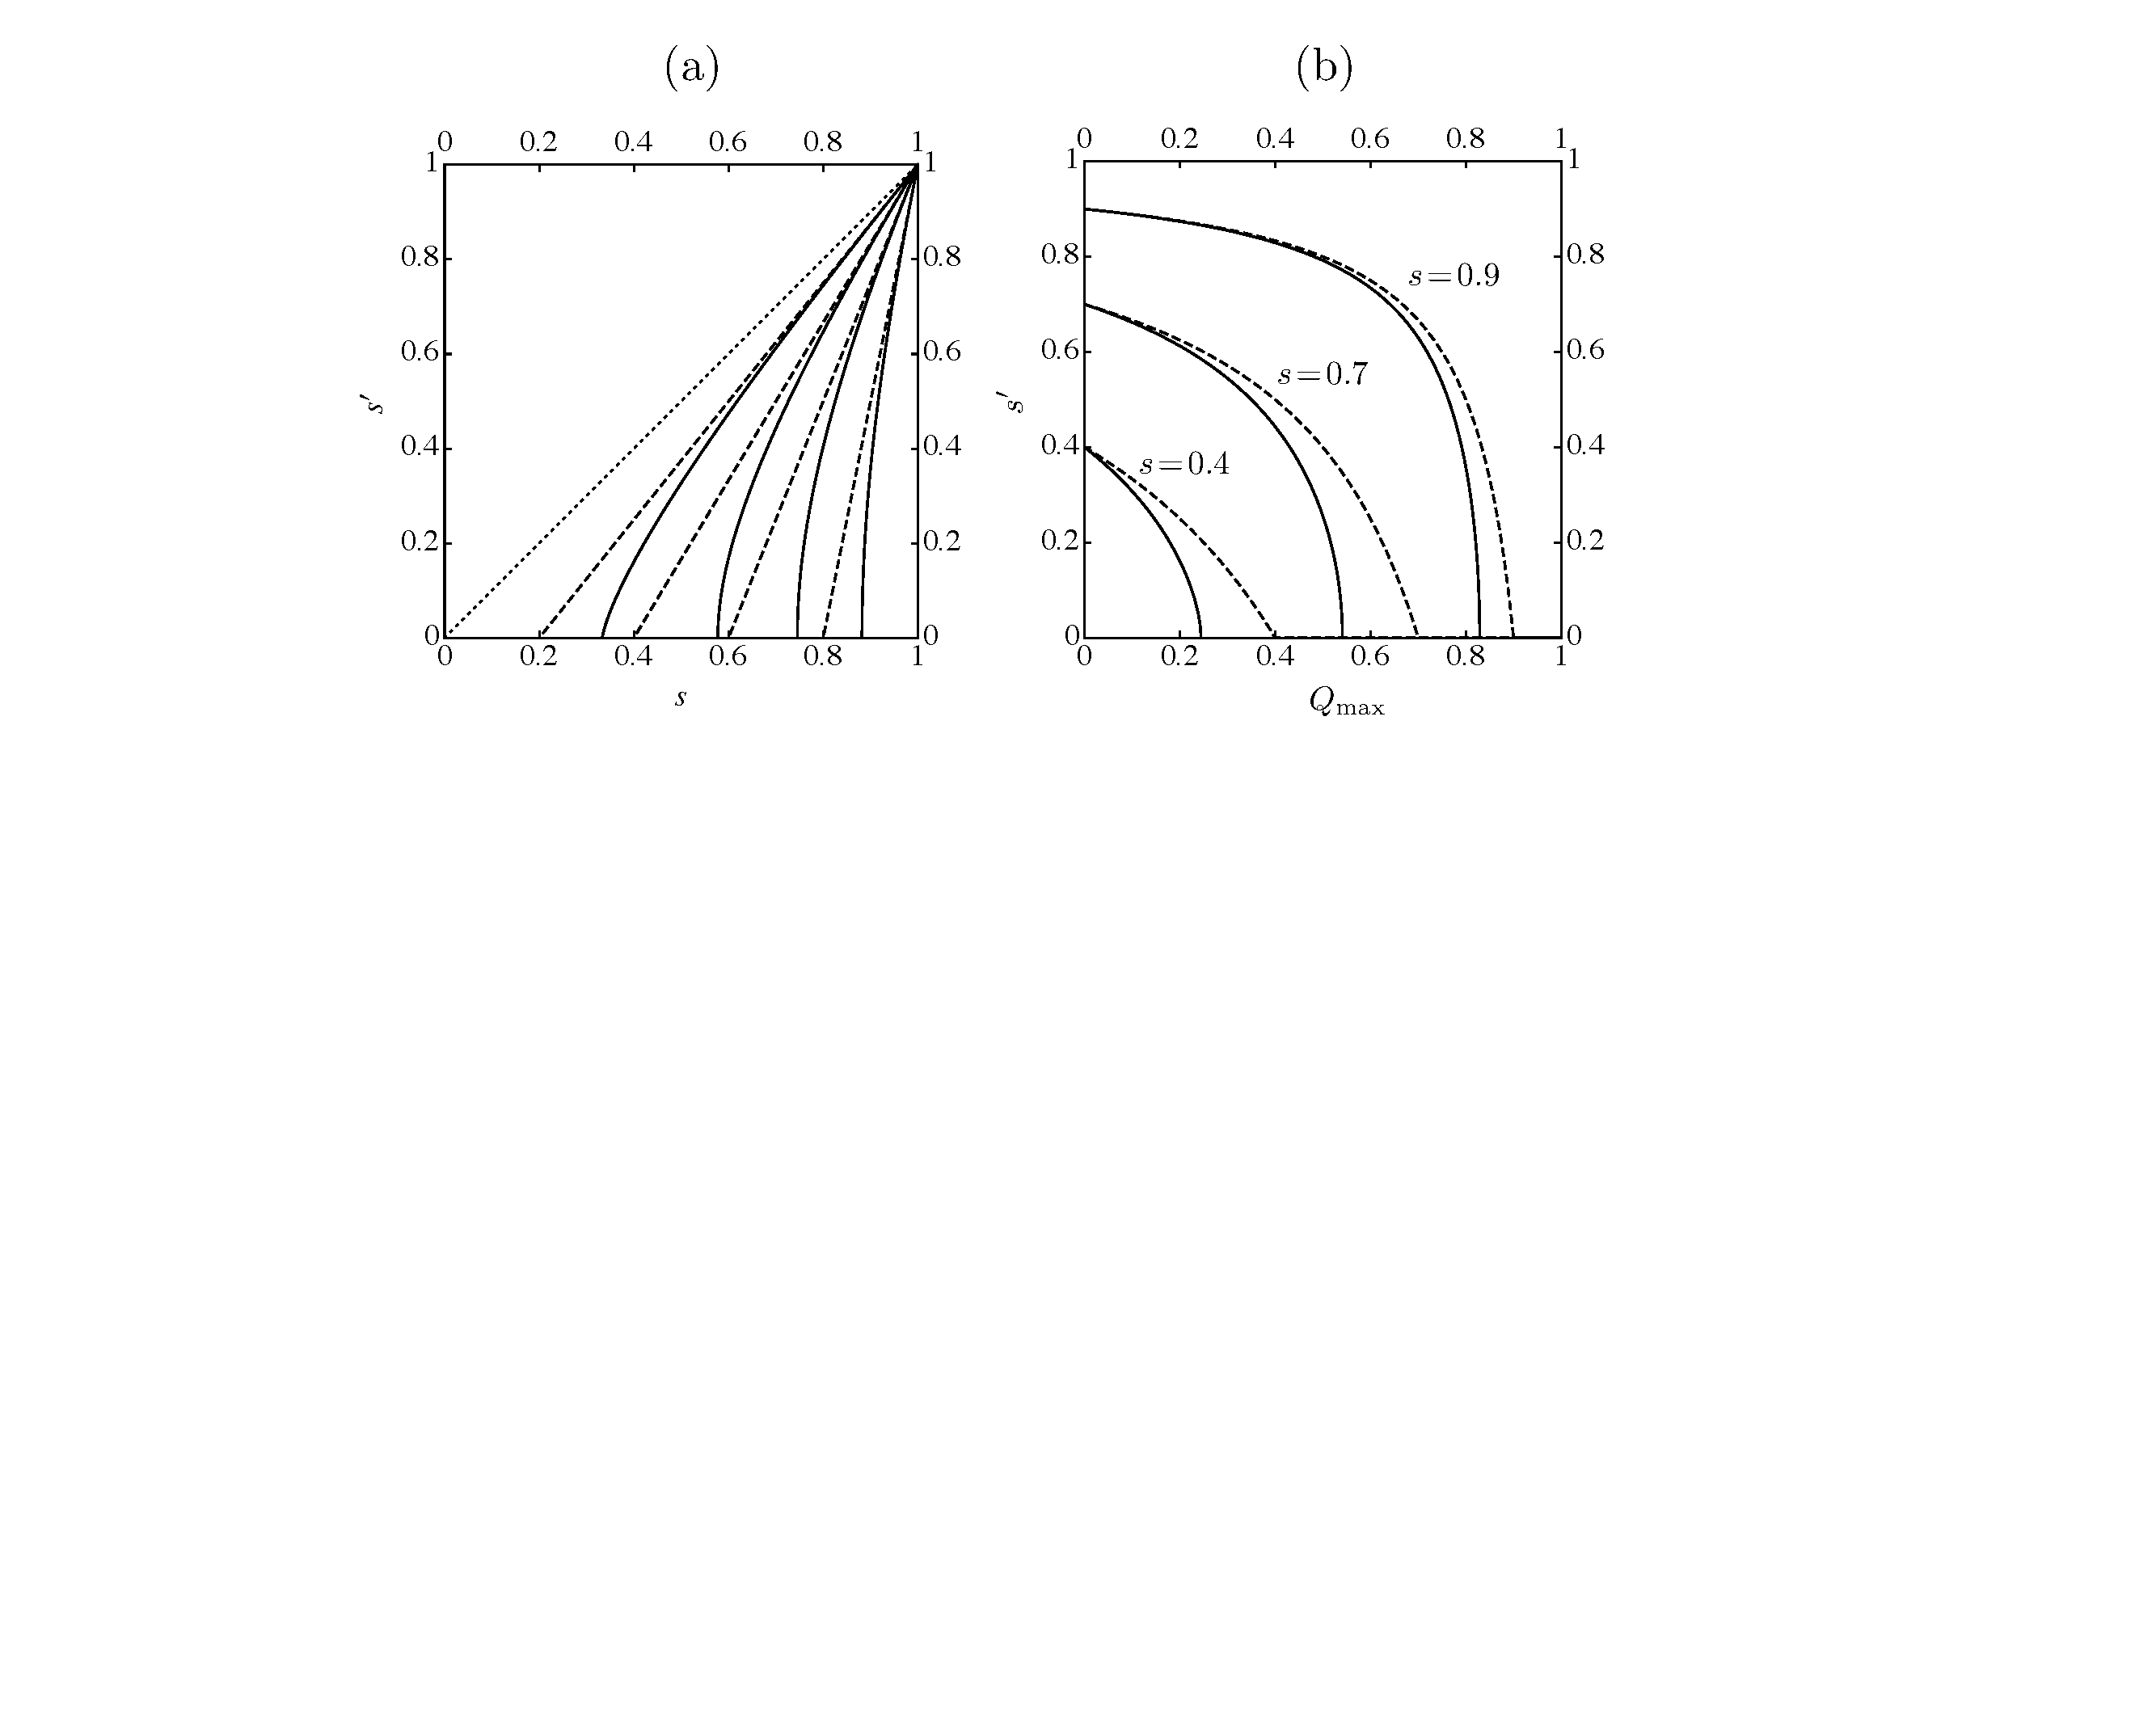
\includegraphics[width=26em]{Separation_F3_4}
   \caption{(a) Plots of $s'$ vs. $s$ for $\eta_1=0.1$ (solid lines) and $\eta_1=0.5$ (straight dashed lines) and for values of the failure rate. From left to right $Q_{\rm max}=0.2$, $0.4$, $0.6$, $0.8$. The dotted line is the (trivial) curve for $Q_{\rm max}=0$, which is the straight line $s'=s$. (b)~Minimum final overlap vs. maximum failure probability for various values of the initial overlap and the same two values of $\eta_1$ used in~(a).\vspace{-1em}
   }
   \label{fig:4}
\end{figure}

Eqs.~(\ref{eb04.05.15-1}) and~(\ref{eb04.05.15-2}) are plotted in Fig.~\ref{fig:4}~(a) for two possible priors: $\eta_1=0.1$ (solid lines) and $\eta_1=0.5$, i.e., for equal priors  (dashed lines). From left to right, the maximum allowed failure rate~$Q_{\rm max}$ is $0.2$, $0.4$, $0.6$ and~$0.8$. We see that for small values of the initial overlap, $s$, one can attain full separation ($s'=0$). Past the critical value,
%%
%\begin{equation}
%s_{\rm cr}=
%\left\{
%\begin{array}{lll}
%\displaystyle {Q_{\rm max}\over\sqrt{1-\Delta^2}}={Q_{\rm max}\over 2\sqrt{\eta_1\eta_2}}&\mbox{if}&\displaystyle Q\le 1-\Delta,\\[1em]
%\displaystyle
%\sqrt{2Q_{\rm max}+\Delta-1\over1+\Delta}
%&\mbox{if}&\displaystyle Q\ge 1-\Delta,
%\end{array}
%\right.
%\end{equation}
%%
%
\begin{equation}
s_{\rm cr}=
\left\{
\begin{array}{lll}
\displaystyle{Q_{\rm max}\over 2\sqrt{\eta_1\eta_2}}&\mbox{if}&\displaystyle Q\le 2\eta_1,\\[1.2em]
\displaystyle
\sqrt{Q_{\rm max}-\eta_1\over\eta_2}
&\mbox{if}&\displaystyle Q\ge 2\eta_1,
\end{array}
\right.
\end{equation}
%
 full separation is no longer possible and~$s'$ increases (quite abruptly for small $\eta_1$). In the region $s<s_{\rm cr}$, the margin $Q_{\rm max}$ is not necessarily saturated,  since the unambiguous discrimination failure probability $Q_{\rm UD}$ is  smaller than $Q_{\rm max}$. For $s\ge s_{\rm cr}$ we necessarily have to saturate the margin, $Q=Q_{\rm max}$. For equal priors (dashed lines) one can obtain the curves in explicit form from Eq.~(\ref{unit cond}) using that $q_1=q_2=Q$:
%
\begin{equation}
s'=
\left\{
\begin{array}{lll}
\displaystyle0 &\mbox{if}& s\le Q_{\rm max},\\[.7em]
\displaystyle
{s-Q_{\rm max}\over 1-Q_{\rm max}}
&\mbox{if}&\displaystyle s\ge Q_{\rm max}.
\end{array}
\right.
\label{tradeoff equal}
\end{equation}
% 
This expression could also be obtained by carefully taking the limit $\Delta\to 0$ in Eqs.~(\ref{eb04.05.15-1})  through~(\ref{eb21.04.15-3}).
The figure clearly shows that separation becomes less demanding as we move away from the equal prior case. For \mbox{$Q_{\rm max}=0$}, i.e., in the deterministic limit, we recover the trivial solution $s'=s$ (dotted line).

\vspace{10em}

\section{Tradeoff between Maximum separation and failure rate}

By solving the system Eq.~(\ref{eb21.04.15-2}) for $Q$ and $s'$ , we obtain a parametric expression for the tradeoff curve $(Q,s')$ in terms of the polar angle $\theta$:
%
%\begin{widetext}
%%%
%%\begin{eqnarray}
%%s'^2&=&\sqrt{1-\Delta^2}\,{\sqrt{1-\Delta^2}(1+s^2)\cos\theta-2s\left(1+\Delta \sin\theta\right)\over(\Delta+\sin\theta)^2} {\sin^2\theta\sec\theta},\label{eb29.04.15-1}\\[.5em]
%%%
%%Q&=&{s\sqrt{1-\Delta^2}+\Delta\,s'^2\cot\theta\over(1-s'^2)\cos\theta}.
%%\label{eb29.04.15-2}
%%\end{eqnarray}
%%%
%%
%\begin{equation}
%s'^2=\sqrt{1-\Delta^2}\left({\sin\theta\over\Delta+\sin\theta}\right)^2{\sqrt{1-\Delta^2}(1+s^2)\cos\theta-2s\left(1+\Delta \sin\theta\right)\over\cos\theta} ;\qquad
%%
%Q={s\sqrt{1-\Delta^2}+\Delta\,s'^2\cot\theta\over(1-s'^2)\cos\theta}.
%\label{tradeoff}
%\end{equation}
%%
%\end{widetext}
%
%
\begin{eqnarray}
s'^2\!&=&\!\sqrt{1\!-\!\Delta^2}\left({\sin\theta\over\Delta\!+\!\sin\theta}\right)^2\nonumber
\\
\!&\times&\!{\sqrt{1\!-\!\Delta^2}(1\!+\!s^2)\!\cos\theta\!-\!2s\!\left(1\!+\!\Delta \sin\theta\right)\over\cos\theta} ,
\label{tradeoff1}\\[.5em]
%
Q&=&\!{s\sqrt{1\!-\!\Delta^2}\!+\!\Delta\,s'^2\!\cot\theta\over(1\!-\!s'^2)\cos\theta}.
\label{tradeoff2}
\end{eqnarray}
%
Note that Eq.~(\ref{tradeoff1}) is an expression for the square of the final overlap. To keep the formula for~$Q$, Eq.~(\ref{tradeoff2}), %, for $Q$, 
short, we use~$s'^2$ as a shorthand for Eq.~(\ref{tradeoff1}).  %in the formula for $Q$ in Eq.~(\ref{tradeoff}). It is understood that one has to substitute the first formula for $s'$. 
%
The range of $\theta$ in Eqs.~(\ref{tradeoff1}) and~(\ref{tradeoff2}) is:
$$
-\arctan\,{s\Delta\over\sqrt{1-\Delta^2}}\le\theta\le\theta_{\rm max},
$$
where the upper limit  of the interval can be written as
%
\begin{equation}
\theta_{\rm max}\!=\!\left\{
\!
\begin{array}{lll}
0&\mbox{if}&\displaystyle \eta_1\!\ge\!{s^2\over1\!+\!s^2},\\[1em]
\displaystyle \!-\!\arccos\!{2s\sqrt{1-\Delta^2}\over1\!-\!\Delta\!+\!s^2(1\!+\!\Delta)}
&\mbox{if}&\displaystyle \eta_1\!\le\!{s^2\over1\!+\!s^2}.
\end{array}
\right.
\label{tradeoff cases}
\end{equation}
%
The lower limit  in the range of allowed $\theta$  can be derived from Eqs.~(\ref{tradeoff1}) and~(\ref{tradeoff2}) by imposing that $Q=0$ at $s'=s$. The upper limit can be derived from Eq.~(\ref{tradeoff1}) by imposing $s'=0$. Once again, we see that a second order phase transition occurs in the limit of full separation: by substituting the first (second) line of Eq.~(\ref{tradeoff cases}) in Eq.~(\ref{tradeoff2}) we obtain $Q=s\sqrt{1-\Delta^2}$\ ($Q=[1-\Delta+s^2(1+\Delta)]/2$), which is the first (second) case in Eq.~(\ref{UD}).

Fig.~\ref{fig:4}~(b) shows various plots of the separation vs. failure-rate tradeoff curve. As in Fig.~\ref{fig:3}, the plots are for~$\eta_1=0.1$ (solid lines) and for equal priors, $\eta_1=\eta_2=0.5$ (dashed lines). For equal priors, there is the explicit formula for the curves given in Eq.~(\ref{tradeoff equal}). Again, we see that as $\eta_1$ gets smaller, departing from the equal prior value~$1/2$, the states can be separated more for the same maximum rate of failure. As $Q_{\rm max}$ increases, the minimum overlap gets smaller, as it should. When~the margin~$Q_{\rm max}$ reaches the unambiguous discrimination value~$Q_{\rm UD}$ we have $s'=0$, attaining full separation. Larger values of~$Q_{\rm max}$ are rather meaningless in this context, since they will never be saturated by an optimal protocol, which requires  a failure rate of only $Q=Q_{\rm UD}$~($<Q_{\rm max}$) to fully separate the input states.

%%%%%%%%%%%%%%%%%%%%%%%%%%%%%%%%%%%%%%%%%%%%%%%%
%%%%%%%%%%%%%%%%%%%%%%%%%%%%%%%%%%%%%%%%%%%%%%%%
%%%%%%%%%%%%%%%%%%%%%%%%%%%%%%%%%%%%%%%%%%%%%%%%
%%%%%%%%%%%%%%%%%%%%%%%%%%%%%%%%%%%%%%%%%%%%%%%%
\chapter{Linear Optical Experimental Realizations}
\section{Reck-Zeilinger Algorithm and Single-Photon Interferometry }
A significant motivation to solving information theory problems using Neumark's theorem is that solutions lend themselves to linear optical implementation.  This implementation requires sources of individual photons, beamsplitters, mirrors, and photodetectors.  In their letter, Reck $et$ $all$ showed that any $N$x$N$ unitary matrix can be reduced to $N(N-1)/2$ beamsplitters acting on $N$ degrees of freedom.  If we allow single photons through a set of beamsplitters to $N$ independent paths, a single photon interferometry device with an appropriate number of optical elements can represent the action of any unitary matrix. A main benefit from seeking a solution using the Neumark setup is that it lends itself to quickly solving for the matrix elements of the unitary, thereby allowing us to express our results
as experimental setups akin to those previously conducted \cite{some experiments}. 

For example, for interpolative discrimination we had three measurement outcomes, meaning dimensionality three, while the pure states can be represented as qubits, thereby requiring a total of three rails, one of which is ancillary and starts in the vacuum state.  The three income ports are in a superposition of zero and/or one photons, corresponding to the orthogonal states~$|0\rangle$, i.e., the vacuum state, $|1\rangle=a_1^\dagger|0\rangle$,  $|2\rangle=a_2^\dagger|0\rangle$ and $|3\rangle=a_3^\dagger|0\rangle$, where~$a_i^\dagger$ is the creation operator of the electromagnetic field in port~$i$, $i=1,2,3$. Similarly, for the output ports we have~$|1'\rangle=a_1'{}^\dagger|0\rangle$,  $|2'\rangle=a_2'{}^\dagger|0\rangle$ and $|3'\rangle=a_3'{}^\dagger|0\rangle$.

%%%%%%%%%%%%%%%%%%%%%%%%%%%%%%%%%%%%%%%%%%%%%%%%
%%%%%%%%%%%%%%%%%%%%%%%%%%%%%%%%%%%%%%%%%%%%%%%%
\section{Implementation of Pure State Interpolative Discrimination}


The main reason to seek a solution using the Neumark setup is because
it lends itself into an optical implementation. This implementation, as we will see,
can be carried out using only linear optical elements (beamsplitters
and a mirror). The possible states are represented by single photons
and several photodetectors will carry out the measurement process at the
output.  

We use a strategy similar to that developed by J.A Bergou \textit{et al.} \cite{BergouImp},
and seek a unitary transformation that
transforms the states as in (2.1) and (2.2), with the qubits in the states
 $|\psi_{1}\rangle=|1\rangle$
, $|\psi_{2}\rangle=\cos\theta|1\rangle+\sin\theta|2\rangle$ 
and assume the ancilla space is empty for the initial preparation,
 i.e., $\alpha_1 = \alpha_2 = 0$:
\begin{align}
U|1\rangle & =\sqrt{p_{1}}|1\rangle+\sqrt{r_{1}}|2\rangle+\sqrt{q_{1}}|3\rangle\\
U(\cos\theta|1\rangle+\sin\theta|2\rangle) & =\sqrt{r_{2}}|1\rangle+\sqrt{p_{2}}|2\rangle+\sqrt{q_{2}}|3\rangle
\end{align}


From these two equations we can read out six of nine elements of the
three by three Unitary matrix, e.g., $\langle 1 | U | 1 \rangle = \sqrt {p_1}$. The rest can be calculated from the
conditions of the unitarity, $U^{T}U=I$.  They are, up to phase,


\begin{equation}
U=\begin{pmatrix}\sqrt{p_{1}} & \frac{\sqrt{r_{2}}-\sqrt{p_{1}}\cos\theta}{\sin\theta} & \pm\frac{\sqrt{\sin^{2}\theta-p_{1}-r_{2}+2\sqrt{p_{1}r_{2}}\cos\theta}}{\sin\theta}\\
\sqrt{r_{1}} & \frac{\sqrt{p_{2}}-\sqrt{r_{1}}\cos\theta}{\sin\theta} & \pm\frac{\sqrt{\sin^{2}\theta-r_{1}-p_{2}+2\sqrt{p_{2}r_{1}}\cos\theta}}{\sin\theta}\\
\sqrt{q_{1}} & \frac{\sqrt{q_{2}}-\sqrt{q_{1}}\cos\theta}{\sin\theta} & \pm\frac{\sqrt{sin^{2}\theta-q_{1}-q_{2}+2\sqrt{q_{1}q_{2}}\cos\theta}}{\sin\theta}
\end{pmatrix}.
\end{equation}

It is worth mentioning that all equations in this section referencing
$r_i$ and $p_i$ are using the optimal values (2.9) and (2.10) derived
in the previous section.

Now that we have a full unitary matrix we want to express it in terms
of linear optical devices. M. Reck \textit{et al.} \cite{Reck}, prove
that any discrete finite-dimensional unitary operator can be constructed
using optical devices. They derive an algorithm which gives the exact
ordering of the beamsplitters and phase shifters. In our work we use
the simplified version of the Reck algorithm given by Y. Sun
$\textit{et al.}$ \cite{Sun} : the operator $U$ is decomposed into
beamsplitters in the order of $U=M_{1}\cdot M_{2}\cdot M_{3}$,
and no phase shifters are needed: 
\begin{align*}
M_{1}&=\begin{pmatrix}\sin\omega_{1} & \cos\omega_{1} & 0\\
\cos\omega_{1} & -\sin\omega_{1} & 0\\
0 & 0 & 1
\end{pmatrix},\\
M_{2}&=\begin{pmatrix}\sin\omega_{2} & 0 & \cos\omega_{2}\\
0 & 1 & 0\\
\cos\omega_{2} & 0 & -\sin\omega_{2}
\end{pmatrix},\\
M_{3}&=\begin{pmatrix}1 & 0 & 0\\
0 & \sin\omega_{3} & \cos\omega_{3}\\
0 & \cos\omega_{3} & -\sin\omega_{3}
\end{pmatrix},\\
\end{align*}

where the coefficients of reflectivity and transmittance are given by $\sqrt{R_{i}}=\sin\omega_{i}$
and $\sqrt{T_{i}}=\cos\omega_{i}$.

All of the beamsplitter coefficients can be derived up to a phase by using just
$U_{31},U_{32},U_{21}$. The sign of the coefficients
is chosen by matching all the elements from the two matrices. The
coefficients are:

\begin{align*}
\cos\omega_{1}&=\sqrt{\frac{r_{1}}{1-q_{1}}},\\
\sin\omega_{1}&=\sqrt{\frac{p_{1}}{1-q_{1}}},\\
\cos\omega_{2}&=\sqrt{q_{1}},\\
\sin\omega_{2}&=\sqrt{1-q_{1}},\\
\cos\omega_{3}&=-\frac{1}{\sqrt{1-q_{1}}}[\frac{\sqrt{q_{2}}-\sqrt{q_{1}}\cos\theta}{\sin\theta}],\\
\sin\omega_{3}&=\frac{\sqrt{\sin^{2}\theta-q_{1}-q_{2}+2\sqrt{q_{1}q_{2}}\cos\theta}}{\sqrt{1-q_{1}}\sin\theta}.\\
\end{align*}

All the terms can be expressed in terms of the fixed failure rate
and fixed a-priori probabilities. Using the optimal relationship between
the individual failure rates $\eta_{1}q_{1}=\eta_{2}q_{2}=Q/2$,$q_{1}=Q/2\eta_{1},q_{2}=Q/2\eta_{2}$
and the optimal expressions of success and error rates the beamsplitters
are
\begin{eqnarray}
M_{1}=\begin{pmatrix}\sqrt{\frac{p_{1}}{1-Q/2\eta_{1}}} & \sqrt{\frac{r_{1}}{1-Q/2\eta_{1}}} & 0\\
\sqrt{\frac{r_{1}}{1-Q/2\eta_{1}}} & -\sqrt{\frac{p_{1}}{1-Q/2\eta_{1}}} & 0\\
0 & 0 & 1\\
\end{pmatrix},\\
M_{2}=\begin{pmatrix}\sqrt{1-Q/2\eta_{1}} & 0 & \sqrt{Q/2\eta_{1}}\\
0 & 1 & 0\\
\sqrt{Q/2\eta_{1}} & 0 & -\sqrt{1-Q/2\eta_{1}}
\end{pmatrix},\\
M_{3}=\begin{pmatrix}1 & 0 & 0\\ 0 & \frac{\sqrt{1-Q_{o}^{2}/4\eta_{1}\eta_{2}-Q/(2\eta_{1}\eta_{2})+QQ_{o}/(2\eta_{1}\eta_{2})}}{\sqrt{(1-Q/2\eta_{1})(1-Q_{o}^{2}/4\eta_{1}\eta_{2})}} & -\frac{\sqrt{Q/2\eta_{2}}-Q_{o}/2\eta_{1}\sqrt{Q/2\eta_{2}}}{\sqrt{(1-Q/2\eta_{1})(1-Q_{o}^{2}/4\eta_{1}\eta_{2})}}\\ 0 & -\frac{\sqrt{Q/2\eta_{2}}-Q_{o}/2\eta_{1}\sqrt{Q/2\eta_{2}}}{\sqrt{(1-Q/2\eta_{1})(1-Q_{o}^{2}/4\eta_{1}\eta_{2})}} & -\frac{\sqrt{1-Q_{o}^{2}/4\eta_{1}\eta_{2}-Q/(2\eta_{1}\eta_{2})+QQ_{o}/(2\eta_{1}\eta_{2})}}{\sqrt{(1-Q/2\eta_{1})(1-Q_{o}^{2}/4\eta_{1}\eta_{2})}} \end{pmatrix}.
\end{eqnarray}
\vspace{0.05in}

An attractive simplification can be acheived by setting $\eta_1 = \eta_2$, the equal apriori condition.  In this case our final unitary matrix can be expressed as
\begin{equation}
U=\begin{pmatrix}\sqrt{p} & \frac{\sqrt{r}-\sqrt{p}Q_{o}}{\sqrt{1-Q_{o}^{2}}} & \sqrt{\frac{Q}{1+Q_{o}}}\\
\sqrt{r} & \frac{[\sqrt{p}-\sqrt{r}Q_{o}]}{\sqrt{1-Q_{o}^{2}}} & \sqrt{\frac{Q}{1+Q_{o}}}\\
\sqrt{Q} & \sqrt{\frac{Q(1-Q_{o})}{1+Q_{o}}} & -\frac{\sqrt{p}+\sqrt{r}}{\sqrt{1+Q_{o}}}
\end{pmatrix}
\end{equation}
By choosing the FRIO this matrix minimizes the error rate and maximizes
the rate of success. Hence, by setting the FRIO to zero we obtain
the setup to the minimum error problem on the other hand setting the
error rate to zero gives the setup of the optimal unambiguous discrimination
where $ $the optimal inconclusive rate is the $Q_{o}=s$. This simplifies
the works of the experimentalists because now they only need one setup
and are not restrained to the extreme points.

The unitary transformation for the Helstrom bound $Q=0$ implementation
can be written using the relations $r=(\frac{\sqrt{r}-\sqrt{p}Q_{o}}{\sqrt{1-Q_{o}^{2}}})^{2}$, $p=(\frac{\sqrt{p}-\sqrt{r}Q_{o}}{\sqrt{1-Q_{o}^{2}}})^{2}$, as

\begin{equation}
U_{ME}=\begin{pmatrix}\sqrt{p} & \sqrt{r} & 0\\
\sqrt{r} & -\sqrt{p} & 0\\
0 & 0 & 1
\end{pmatrix}.
\end{equation}

Clearly only the $M_1$ beamsplitter is necessary to implement the ME state discrimination.

On the other extreme, the unitary transformation for the optimal UD
bound $(P_{E}=0)$ implementation becomes:

\begin{equation}
U_{UD}=\begin{pmatrix}\sqrt{p} & -\frac{\sqrt{p}Q_{o}}{\sqrt{1-Q_{o}^{2}}} & \sqrt{\frac{Q_{0}}{1+Q_{o}}}\\
0 & \frac{\sqrt{p}}{\sqrt{1-Q_{o}^{2}}} & \sqrt{\frac{Q_{o}}{1+Q_{o}}}\\
\sqrt{Q_{0}} & \sqrt{\frac{Q_{o}(1-Q_{o})}{1+Q_{o}}} & -\sqrt{\frac{1-Q_{o}}{1+Q_{o}}}
\end{pmatrix}.
\end{equation}
All three beamsplitters are still necessary for a general UD measurement.  This is because the measurement is essentially two-step:  in the first step we attempt to orthogonalize the states, and upon succeeding we perform a projective measurement.



%%%%%%%%%%%%%%%%%%%%%%%%%%%%%%%%%%%%%%%%%%%%%%%%
%%%%%%%%%%%%%%%%%%%%%%%%%%%%%%%%%%%%%%%%%%%%%%%%
\section{Implementation of State Separation }

In this section we derive a similar implementation of optimal separation, sketched in Fig.~\ref{fig:5}.The implementation uses only  two beam splitters, M1 and~M2. The measurements are carried out  by three photodetectors. 


We can choose several different representations for our input states.  The first is such that one state is parallel to a basis vector, allowing for the unitary transformation to be represented, using Eqs.~(\ref{U1}) and~(\ref{U2}), as
\begin{eqnarray}
U |1\rangle&=&\sqrt{p_1}|1'\rangle+\sqrt{q_1}|3'\rangle,\label{U1 impl}\\[.2em]
U\left( s|1\rangle+\sqrt{1-s^2} |2\rangle\right)&=&\sqrt{p_1}\left( s'|1'\rangle+\sqrt{1-s'^2} |2'\rangle\right)+\sqrt{q_1}|3'\rangle,\label{U2 impl}
\end{eqnarray}

%
which corresponds to the choice: $|\psi_1\rangle|0\rangle=|1\rangle$, $|\psi_2\rangle|0\rangle=s|1\rangle+\sqrt{1-s^2}|2\rangle$, $|\psi'_1\rangle|\alpha_1\rangle=|1'\rangle$, $|\psi'_2\rangle|\alpha_2\rangle=s'|1'\rangle+\sqrt{1-s'^2}|2'\rangle$ and $|\phi\rangle|\alpha_0\rangle=|3'\rangle$.  The third rail always

 So, input port $3$ is always in the vacuum state. The detection of a photon in the output port $3'$ signals that separation failed. The state~$|\psi_2\rangle$ can be produced  in a standard way by sending a photon into a beam splitter with suitable transmission and reflection coefficients.
%
\begin{figure}[h] %  figure placement: here, top, bottom, or page
   \centering
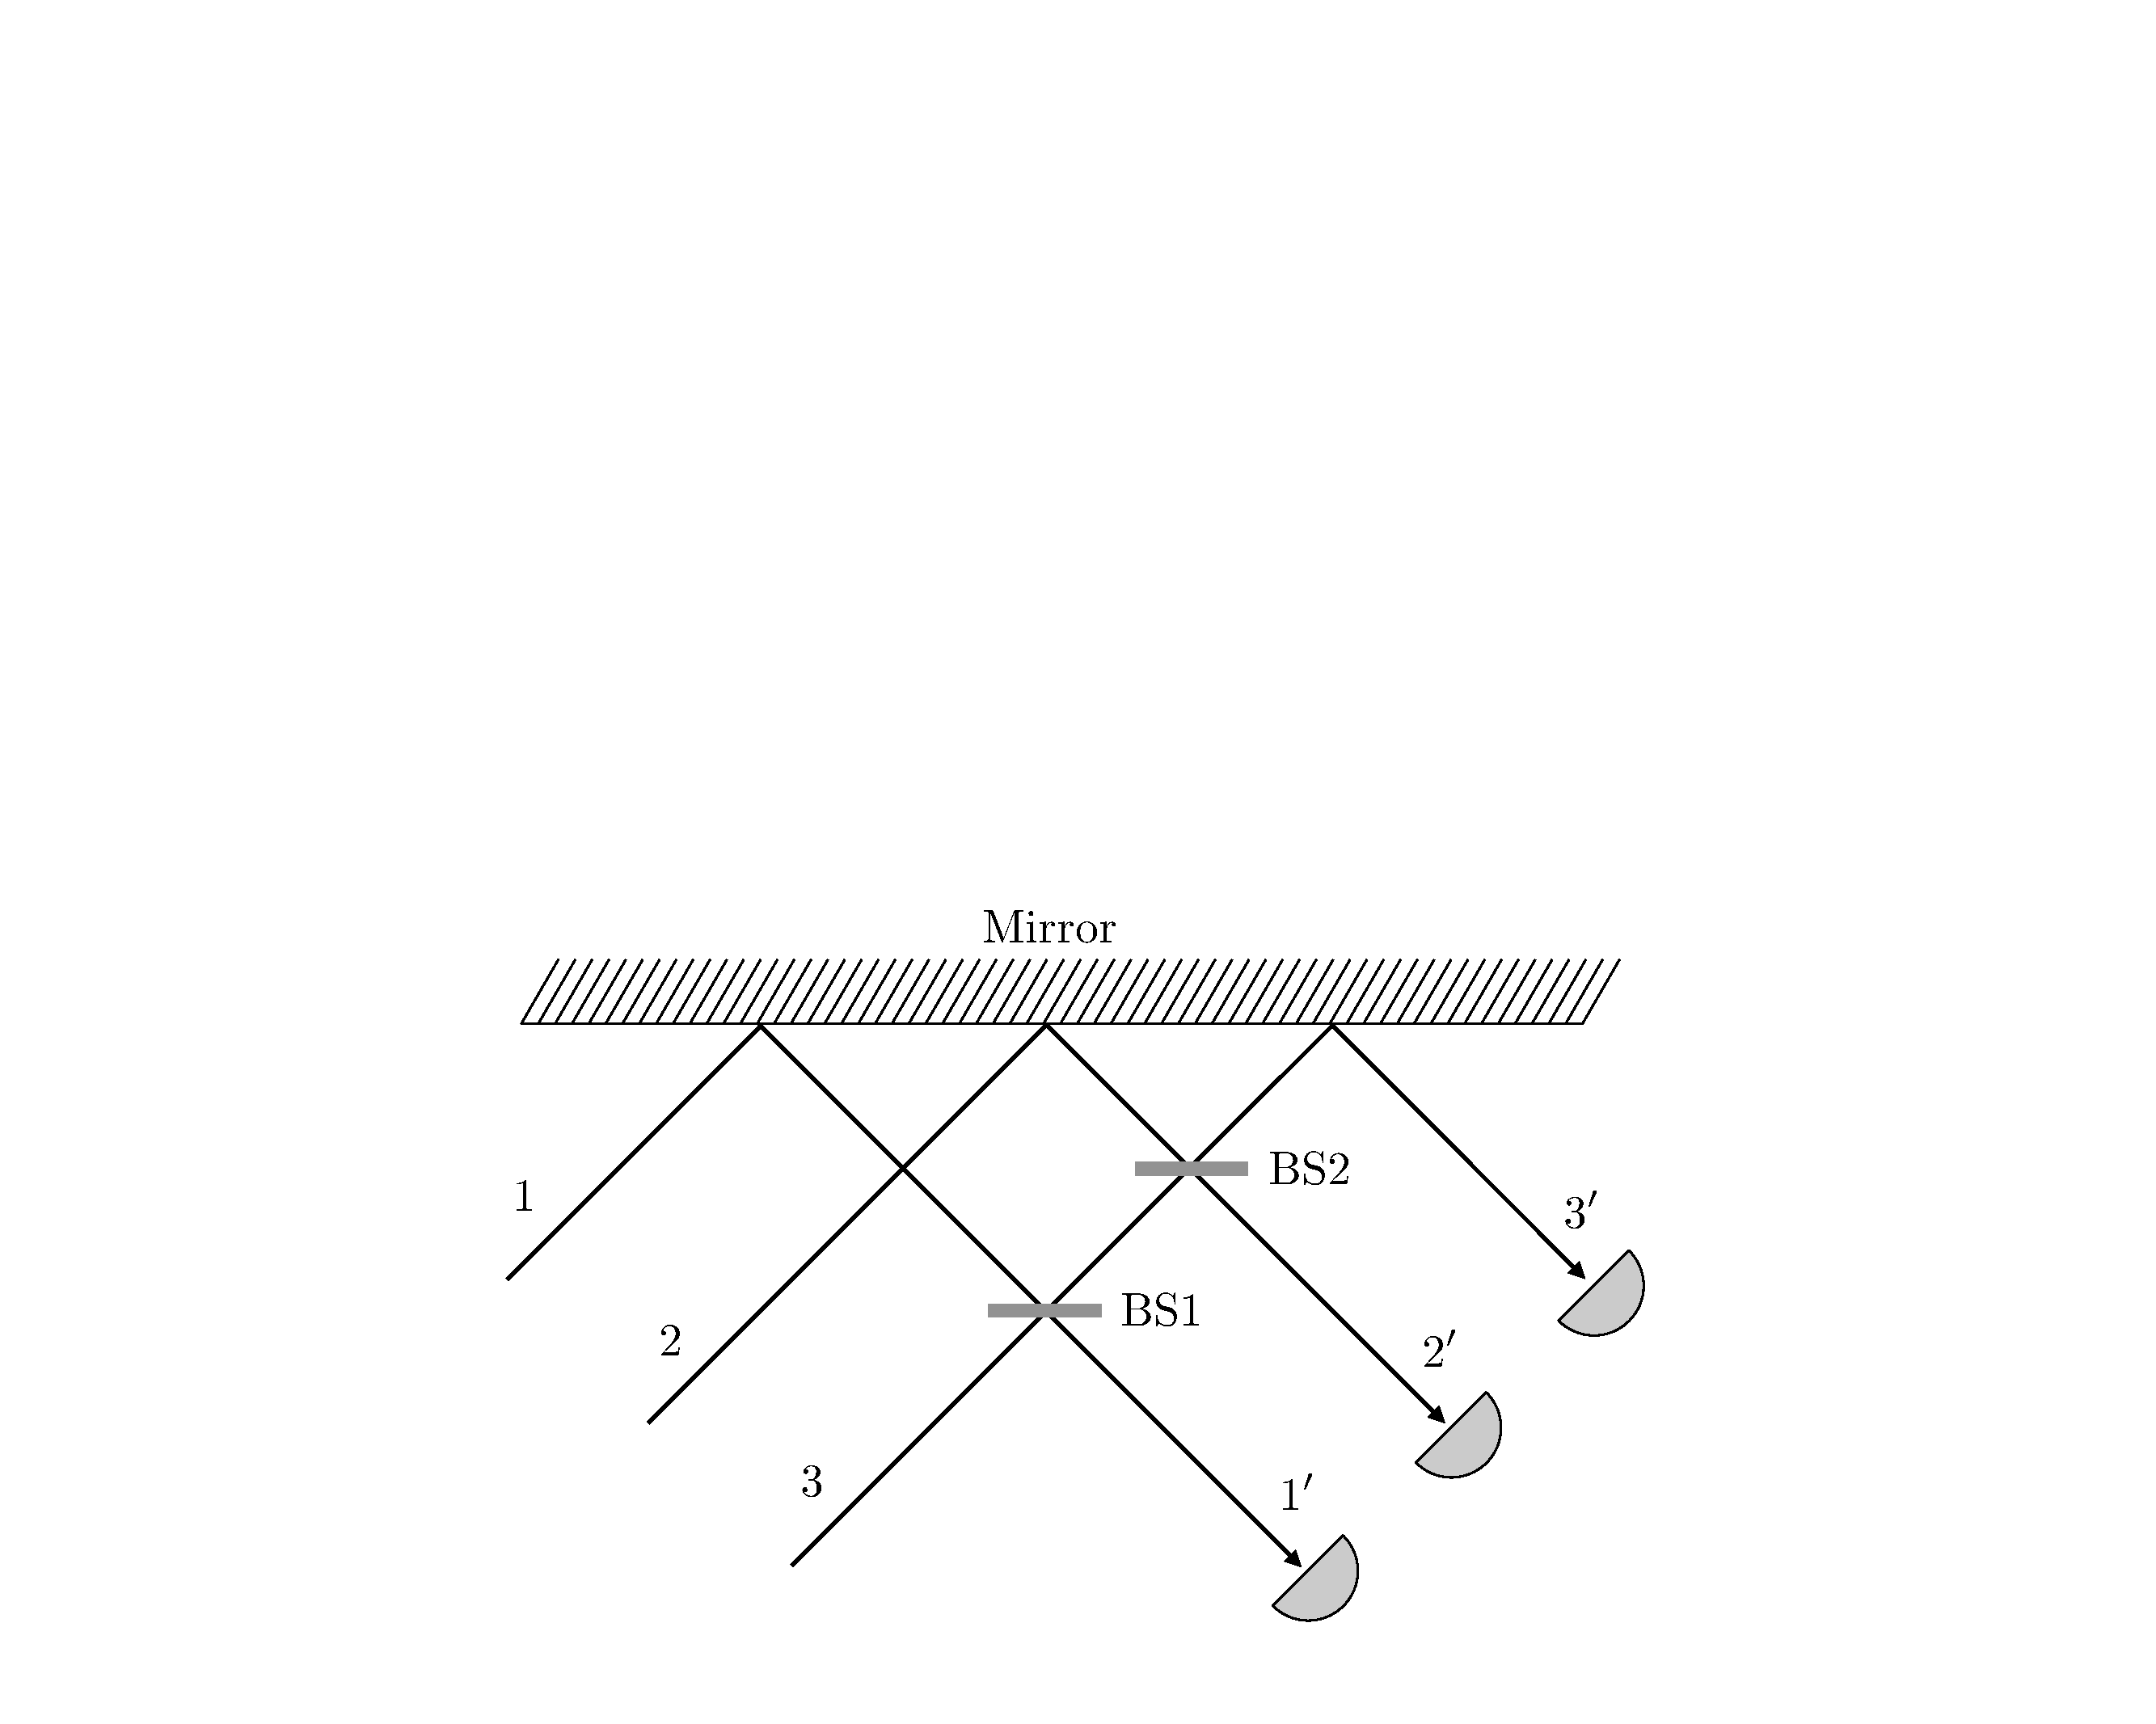
\includegraphics[width=18em]{Separation_F5}\vspace{2em}
   \caption{Six-port linear optics implementation of a proof-of-principle separation protocol. The transmission (reflexion) coefficients of the beamsplitters, BS1 and BS2 are given by the (off-)diagonal entries of the matrices in Eqs.~(\ref{M1}) and~(\ref{M2}), respectively. The input states are feed through ports $1$ and $2$ as a superposition of zero and one photons in each port. The separated states are output through ports $1'$ and $2'$. Port $3$ is in the vacuum state. A click in the photodetector placed in port $3'$ signals failure.}
   \label{fig:5}
\end{figure}
%

For simplicity, we consider equal prior probabilities $\eta_1=\eta_2=1/2$, but the same setup can be used in the general case. As mentioned above, for equal priors we must have $q_1=q_2=Q$ and $p_1=p_2=1-Q$ and the unitarity condition Eq.~(\ref{unit cond}) can be solved explicitly. The solution is given by $Q=Q_{-1}$ in Eq.~(\ref{Q's}). Substituting in Eqs.~(\ref{U1 impl}) and~(\ref{U2 impl}) we obtain two columns of the matrix of the unitary transformation $U$ in the basis introduced above. The remaining  column can be easily obtained imposing unitarity. After some algebra we have
%
\begin{equation}
[U]=\begin{pmatrix}\sqrt{\frac{1-s}{1-s'}} & -\frac{s-s'}{\sqrt{(1-s')(1+s)}} & -\sqrt{\frac{(1+s')(s-s')}{(1-s')(1+s)}}\\[.7em]
0 & \sqrt{\frac{1+s'}{1+s}} & -\sqrt{\frac{s-s'}{1+s}}\\[.7em]
\sqrt{\frac{s-s'}{1-s'}} & \sqrt{\frac{(1-s)(s-s')}{(1+s)(1-s')}} & \sqrt{\frac{(1-s)(1+s')}{(1-s')(1+s)}}
\end{pmatrix}.
\end{equation}
%
Using~\cite{reck,BergouImp} we can write $U$ as the product $U=M_1 M_2$, where the matrices of $M_1$ and $M_2$  are
%
\begin{eqnarray}
{}[M_1]&=&\begin{pmatrix}\sqrt{\frac{s-s'}{1-s'}} & 0 & \sqrt{\frac{s-s'}{1-s'}}\\
0 & 1 & 0\\
\sqrt{\frac{s-s'}{1-s'}} & 0 & -\sqrt{\frac{s-s'}{1-s'}}
\end{pmatrix},\label{M1}\\[1em]
{}[M_2]&=&
\begin{pmatrix}1 & 0 & 0\\
0 & \sqrt{\frac{1+s'}{1+s}} & -\sqrt{\frac{s-s'}{1+s}}\\
0 & -\sqrt{\frac{s-s'}{1+s}} & -\sqrt{\frac{1+s'}{1+s}}
\end{pmatrix}.
\label{M2}
\end{eqnarray}
%
%
%\begin{equation}
%[U]=\begin{pmatrix}\sqrt{\frac{s-s'}{1-s'}} & 0 & \sqrt{\frac{s-s'}{1-s'}}\\
%0 & 1 & 0\\
%\sqrt{\frac{s-s'}{1-s'}} & 0 & -\sqrt{\frac{s-s'}{1-s'}}
%\end{pmatrix}\\
%\begin{pmatrix}1 & 0 & 0\\
%0 & \sqrt{\frac{1+s'}{1+s}} & -\sqrt{\frac{s-s'}{1+s}}\\
%0 & -\sqrt{\frac{s-s'}{1+s}} & -\sqrt{\frac{1+s'}{1+s}}
%\end{pmatrix}
%\end{equation}
%
We immediately recognize that the transformation $M_1$ and $M_2$ can be implemented with beamsplitters, labeled in Fig.~\ref{fig:5} by  BS1 and BS2, respectively. The corresponding matrix elements provide the transmission (diagonal) and reflection  (off-diagonal) coefficients of these beamsplitters.

The degree of separation attained by the protocol can be certified by statistical analysis of the photon counts in the detectors placed in the ports $1'$ and $2'$, whereas those in the detector placed in port $3'$ provide the failure rate~$Q$. 

We should stress that this is a proof-of-principle protocol. The transformation $U$ is design with the only aim of decreasing the overlap of the initial states, and no other communication or computational task is intended to be carried out by this implementation. However, we might consider removing the detectors in $1'$ and $2'$ and feed the output states into some other optical setup for further processing. Hence, this implementation can be thought of as a separation module in a larger experimental setup.

%%%%%%%%%%%%%%%%%%%%%%%%%%%%%%%%%%%%%%%%%%%%%%%%
%%%%%%%%%%%%%%%%%%%%%%%%%%%%%%%%%%%%%%%%%%%%%%%%
\section{Implementation of Probabilistic Approximate Cloning}
In order to clone N copies of state $\ke {\psi}$ approximately we need N+1 ports for our interferometer.
This results in very complicated applications of the R-Z algorithm when N becomes large.  We therefore
demonstrate the solution on $1 \rightarrow 2$ cloning with equal prior probabilities.  If we perform this
operation as a one-shot measurement we would need a 5x5 unitary.

However we can probabilistically optimally separate the two input states, then apply a cloning unitary to make the
desired copies.  Since we know the optimal relationship between the inpupt and output overlaps from the previous chapter, the first step is choosing the desired final overlap and failure rate. Given the final overlap we optimally deterministically transform these states into the clones.  This reduces the complexity of the problem sinces now we are working with 4x4 and 3x3 matricies.  It was realized a shorter realization of separation exists for a different choice of basis states.  We demonstate in detail next.

However we can probabilistically optimally separate the two input states using the results of the previous section,
then apply a cloning unitary to make the desired copies.  Since we know the optimal relationship
between input and ouput overlaps from the previous chapter, the first step is choosing the desired final overlap
and failure rate.  Given the final overlap we optimally deterministically transform these states into the clones.
This reduces the complexity of the problem since now we are working with a 4x4 matrix.  
%%%%%%%%%%%%%%%%%%%%%%%%%%%%%%%%%%%%%%%%%%%%%%%%
%%%%%%%%%%%%%%%%%%%%%%%%%%%%%%%%%%%%%%%%%%%%%%%%
\subsection{Shorter Separation Implementation}
We start by choosing the same unitarity equations as before, instead choosing $\ke 0$ as that for failure,
\begin{eqnarray}
U\ke {\psi_1} = \sqrt{p_1}\ke{\phi_1}+ \sqrt{q_1}\ke{0}\\
U\ke {\psi_2} = \sqrt{p_2}\ke{\phi_2}+ \sqrt{q_2}\ke{0}
\end{eqnarray}
but now our states are chosen symmetrically as $\ke {\psi_1} = c_1 \ke{1} + s_1 \ke{2}$, $\ke {\psi_2} = c_1 \ke{1} - s_1 \ke{2}$,
$\ke {\phi_1} = c_2 \ke{1} + s_2 \ke{2}$, and $\ke {\phi_2} = c_2 \ke{1} - s_2 \ke{2}$.  
For general a-priori probabilities the basis of the
output states could be rotated, along with a changed overlap.  However for the equal-priors case this rotation is non-existant, and the symmetry
between the states is preserved. By sandwiching the unitary with the basis states we are able to write the equations for six of its nine elements as
\begin{eqnarray}
\br 0 U \ke {\psi_1} &=&c_1 U_{01} + s_1 U_{02} = \sqrt{q_1},\\
\br 0 U \ke {\psi_1} &=&c_1 U_{11} + s_1 U_{12} = c_2 \sqrt{p_1},\\
\br 0 U \ke {\psi_1} &=&c_1 U_{21} + s_1 U_{22} = s_2\sqrt{p_1},
\end{eqnarray}
and
\begin{eqnarray}
\br 0 U \ke {\psi_2} &=& c_1 U_{01} - s_1 U_{02} = \sqrt{q_2},\\
\br 1 U \ke {\psi_2} &=&c_1 U_{11} - s_1 U_{12} = c_2\sqrt{p_2},\\
\br 2 U \ke {\psi_2} &=& c_1 U_{21} - s_1 U_{22} = -s_2\sqrt{p_2}.
\end{eqnarray}
We can solve the the two sets of equations pairwise for the first six matrix elements, giving
\begin{equation}
{}[U]=
\begin{pmatrix}\bullet & \frac{\sqrt{q_1}+\sqrt{q_2}}{2c_1} & \frac{\sqrt{q_1}-\sqrt{q_2}}{2s_1}\\
\bullet &\frac{c_2(\sqrt{p_1}+\sqrt{p_2})}{2c_1} & \frac{c_2(\sqrt{p_1}-\sqrt{p_2})}{2s_1} \\
\bullet & \frac{s_2(\sqrt{p_1}-\sqrt{p_2})}{2c_1} & \frac{s_2(\sqrt{p_1}+\sqrt{p_2})}{2s_1} 
\end{pmatrix}.
\end{equation}

  Applying the unitarity constraint
$U^\dagger U = I$ can us nine equations for the remaining three uknown elements.  However, using that the probability of success and failure for each state is equal in the equal prior probability case,$p_1 = p_2$ and $q_1 = q_2$, and that when $\eta_1 = \eta_2$ we have the separation solution $p = \frac{\bk{\psi_1}{\psi_2}-1}{\bk{\phi_1}{\phi_2}-1}$, we can simplifying the matrix to

\begin{equation}
{}[U]=
\begin{pmatrix}\bullet & \frac{\sqrt{s_2^2-s_1^2}}{c_1s_2} & 0\\
\bullet &\frac{c_2s_1}{c_1s_2} & 0 \\
\bullet & 0 & 1.
\end{pmatrix}
\end{equation}

This lets us choose the final elements to be consistent with the operation of only a single beam splitter.
implying we can choose the remaining elements to be

\begin{equation}
{}[U]=
\begin{pmatrix}\frac{c_2s_1}{c_1s_2}& \frac{\sqrt{s_2^2-s_1^2}}{c_1s_2} & 0\\
-\frac{\sqrt{s_2^2-s_1^2}}{c_1s_2} &\frac{c_2s_1}{c_1s_2} & 0 \\
0 & 0 & 1
\end{pmatrix}
\end{equation}
\subsection{Deterministic Cloning Implementation}
The unitary transformation
for the second step is
\begin{eqnarray}
U\ke {\phi_1} \ke 0 = \ke{\xi_1}\ke{\xi_1}\\
U\ke {\phi_2} \ke 0 = \ke{\xi_2}\ke{\xi_2}
\end{eqnarray}
where 
$\ke {\xi_1} = c_3 \ke{1} + s_3 \ke{2}$ and
$\ke {\xi_1} = c_3 \ke{1} - s_3 \ke{2}$
Following a similar procedure we choose the basis states $ \ke {00}$,$ \ke {10}$,$ \ke {01}$, and$ \ke {11}$,
giving us the final unitary as 
\begin{equation}
{}[U]=
\begin{pmatrix} \frac{c_3^2}{c_2} &0 & 0 &\frac{s_3^2}{c_2}\\
0 &\frac{c_3 s_3}{s_2} &-\frac{c_3 s_3}{s_2}&0 \\
0 &\frac{c_3 s_3}{s_2} &\frac{c_3 s_3}{s_2}&0 \\
\frac{s_3^2}{c_2} & 0&0&\frac{c_3^2}{c_2}
\end{pmatrix}
\end{equation}

This is clearly the action of two separate beam splitters $M_{14}$ and $M_{23}$ such that
\begin{eqnarray}
{}[M_{14}]=\frac{1}{c_2}
\begin{pmatrix}{c_3^2} &s_3^2\\
 {s_3^2}&{c_3^2}
\end{pmatrix}
{}[M_{23}]=\frac{c_3 s_3}{s_2}
\begin{pmatrix}1 &1 \\
-1 & 1
\end{pmatrix}
\end{eqnarray}
%%%%%%%%%%%%%%%%%%%%%%%%%%%%%%%%%%%%%%%%%%%%%%%%
%%%%%%%%%%%%%%%%%%%%%%%%%%%%%%%%%%%%%%%%%%%%%%%%
%%%%%%%%%%%%%%%%%%%%%%%%%%%%%%%%%%%%%%%%%%%%%%%%
%%%%%%%%%%%%%%%%%%%%%%%%%%%%%%%%%%%%%%%%%%%%%%%%
\chapter{Multi-Step Measurements and Information Loss}

%%%%%%%%%%%%%%%%%%%%%%%%%%%%%%%%%%%%%%%%%%%%%%%%
%%%%%%%%%%%%%%%%%%%%%%%%%%%%%%%%%%%%%%%%%%%%%%%%


\section{Measure and Prepare}
\section{Prepare and Measure}

%%%%%%%%%%%%%%%%%%%%%%%%%%%%%%%%%%%%%%%%%%%%%%%%
%%%%%%%%%%%%%%%%%%%%%%%%%%%%%%%%%%%%%%%%%%%%%%%%
%%%%%%%%%%%%%%%%%%%%%%%%%%%%%%%%%%%%%%%%%%%%%%%%
%%%%%%%%%%%%%%%%%%%%%%%%%%%%%%%%%%%%%%%%%%%%%%%%
\chapter{Appendix}
\section{Relationship between Mixed State ME Detection Strategies}

An interesting problem we considered is the relationship between the discrimation of mixed states with noise and the subspace discrimination problem.  Specifically, solving the Minimum Error case of both problems we get similar answers:

For 
\[ \rho_1 = p \ke {\psi_1} \br {\psi_1}  + \frac{(1-p)}{2} I\] 
and
\[ \rho_1 = d \vert \psi_2 \rangle \langle \psi_2 \vert + \frac{(1-d)}{2} I\]
the ME solution gives 
\[P_e= \frac{1}{2}(1 - Tr \abs{\Lambda})\]
where the solution depends on the characteristic equation 
\[ \lambda^2 - b \lambda + c = 0\]
\[b = \eta_1 -\eta_2 \]
and
\[c = [ \frac{(\eta_1-\eta_2)^2 -(\eta_1p - \eta_2d)^2}{4} -pd \eta_1\eta_2sin^2\theta]\]
The two solutions depend on the positivity of c, the sum of the eigenvalues for $c<0$ is
\[\sum \abs {\lambda_i} = \sqrt{b^2-4c}\]
And the sum of the eigenvalues for $c \geq 0$ is
\[\sum \abs {\lambda_i} =b\]
The b solution gives \[P_e= \frac{1}{2}(1 - Tr \abs{\Lambda}) = \frac{1}{2}(1 -\abs{b})\] 
where assuming $\eta_1 \geq \eta_2$ we get 
\[ P_e = \eta_2\] 
or we simply guess the more likely state.
The $\sqrt{b^2-4c}$ solution gives 
\[P_e= \frac{1}{2}(1 - \sqrt{b^2-4c}) =  \frac{1}{2}(1 - \sqrt{ (\eta_1 p - \eta_2 d)^2 + 4 p d \eta_1 \eta_2 sin^2 \theta)})\]
This solution may not seem remarkable but it is very closely related to the subspace ME solution:
For subspaces where $\rho_1 = \sum r_i \vert r_i \rangle \langle r_i \vert $ and $\rho_2 = \sum s_i \vert s_i \rangle \langle s_i \vert$ with $ \langle r_i \vert s_j \rangle = \delta_{ij} cos \theta_i$
we got the error rate with failure to be
\[P_{e,i}= \frac{1}{2}( \eta_i-Q_i - \sqrt{(\eta_i-Q_i)^2 - (Q_{0,i} - Q_i)^2}),\]
where $\eta_i = \eta_1 r_i + \eta_2 s_i$ and  $Q_{0,i} = 2 \sqrt{\eta_1 r_i\eta_2 s_i}cos\theta_i$.
Setting $Q_i = 0$ we get
\[P_{e,i}= \frac{1}{2}( \eta_i - \sqrt{\eta_i^2 -Q_{0,i}^2}).\]
Let's look at the square root in this expression:
\[ \eta_i^2 -Q_{0,i}^2 = (\eta_1 r_i +\eta_2 s_i)^2 - 4 \eta_1 r_i\eta_2 s_i cos^2\theta_i =   (\eta_1 r_i -\eta_2 s_i)^2 + 4 \eta_1 r_i\eta_2 s_i sin^2\theta_i\]
If we simply call $ r_i = p$ and $s_i = d$ for some subspace then we reproduce the square-root term of the previous solution! This leads us to believe that the problems are very closely related.


%%%%%%%%%%%%%%%%%%%%%%%%%%%%%%%%%%%%%%%%%%%%%%%%
%%%%%%%%%%%%%%%%%%%%%%%%%%%%%%%%%%%%%%%%%%%%%%%%
%%%%%%%%%%%%%%%%%%%%%%%%%%%%%%%%%%%%%%%%%%%%%%%%
%%%%%%%%%%%%%%%%%%%%%%%%%%%%%%%%%%%%%%%%%%%%%%%%
\section{Appendix 2: Lagrange Multipliers}




\bibliographystyle{unsrt}
\bibliography{/Users/ashehu/Desktop/mendeley}

\end{document}
